
\documentclass[11pt,a4paper,twoside,greek]{report}

%%%%%%%%%%%%%%%%%%%%%%%%%%%%%%%%%%%%%%%%%%%%%%%%%%%%%%%%%%%%%%%%%%%%%%%%%%
%%%%%%%%%%%%%%%%%%%%%%%%%%%%%%   PACKAGES   %%%%%%%%%%%%%%%%%%%%%%%%%%%%%%
%%%%%%%%%%%%%%%%%%%%%%%%%%%%%%%%%%%%%%%%%%%%%%%%%%%%%%%%%%%%%%%%%%%%%%%%%%
\usepackage[french]{babel} % Babel est un package qui permet d'obtenir des documents en plusieurs langues, en respectant les typographies nationales, en affichant automatiquement les titres (comme « table des matières », « index », etc) dans la langue choisie, etc.  On peut aussi utiliser babel pour écrire un document en plusieurs langues. Pour cela, il faut lui donner en option la liste de toutes les langues qui seront utilisées en plaçant en dernier la langue principale du document. Pour alterner entre les langues, on utilise la commande : \selectlanguage{nom-de-la-langue}
%\usepackage{standalone}
\usepackage{graphicx}
\usepackage{numprint} % de regrouper les milliers avec la commande \nombre{}
%\usepackage[utf8]{inputenc} % L'inclusion de ce package permet d'utiliser des sources LaTeX contenant des caractères accentués. L'option [latin1]  précise que l'encodage des fichiers est iso-latin1 ou iso iso-8859-1. En effet, sans cette extension, il est nécessaire d'utiliser une syntaxe particulière pour l'affichage des accents. --> Pas nécéssaire en UTF-8
\usepackage{comicneue} % Pour avoir des polices comicneuesur tout le document. Beaucoup plus jolie et agréable à lire
\usepackage[T1]{fontenc} % Permet de spécifier à LaTeX l'utilisation du codage de caractères T1, nouvelle norme LaTeX non utilisée par défaut pour des raisons de compatibilité avec les anciens documents LaTeX.
%\usepackage[francais]{layout} % Est une sorte de bibiothèque de fonction contenant la fonction utile "\layout" qui dessine la structure physique du documents et indique leurs dimensions.
\usepackage{amssymb} % Permet d'utiliser différents symbôles mathématiques.
\usepackage[fleqn]{amsmath} % Permet d'utiliser différents environnements propices aux maths. L'option "fleqn" permet de ne pas centrer l'environnement "align" en conjnction avec la commande \setlength{\mathindent{0pt}}
\usepackage{ulem} % Ce package permet de faire différents types de sous ou sur-lignements. (Comme le double souslignements par exemple).
\usepackage{fancyhdr}  %package pour en-tetes et pied de pages
\usepackage{sectsty} % Permet de faire des modifications de police dans diverses sections des "headings" (cf. modif presentation de la page)
%\usepackage{titlesec}
\usepackage[svgnames,table]{xcolor}   % Permet de définir des nouvelles couleurs (peut-être aussi d'utiliser les couleurs en général)
\usepackage{color}   % Permet de définir des nouvelles couleurs (peut-être aussi d'utiliser les couleurs en général)
\usepackage{lastpage} % Permet à Latex d'identifier la dernière page du document avec la commande "\"
\usepackage[inline]{enumitem} % Permet de préciser des options lors de la déclaration de l’environnement d’une liste à puces
% \usepackage{enumerate} % Permet de faire des liste numérotées avec des i) ; ii) etc... 
\usepackage{shadowtext} % Permet de faire du text avec des ombres
%\usepackage{showframe} % Permet de montrer les marges du document
\usepackage{blindtext} % permet de générer un text avec la commande "\blindtext" afin de tester des macros et autres environnements
\usepackage{tikz} % Permet de faire des dessins avec les commandes Tikz
%\usepackage{auto-pst-pdf}

%\usepackage{pstricks,pst-plot,pstricks-add}

\usepackage{pst-func}
%\usepackage{fourier} % Change la police (assez joli) et permet de faire le sympbole attention: \danger
\usepackage{bold-extra}
%\usepackage{fontspec} % Package pour le polices de caractères
\usetikzlibrary{shapes} %Shape library, used to define shapes other than rectangle, circle and co-ordinate. The following additional types are available: geometric shapes, either named shapes (star, diamond, etc.) or polygons of specified side numbers; symbol shapes, e.g. "forbidden sign" as used in No Smoking signs; "multipart" shapes, with "multiple (text) parts"; and finally, "misc" shapes which "do not fit in the previous categories", such as strikethrough crosses.
\usetikzlibrary{shadows.blur}
\usepackage{bm} % permet de faire des symbole mathématique en gras avec \boldsymbol{}
\usepackage[thicklines]{cancel}
%\usepackage{phantom}
\usepackage{calc}
\usepackage{multicol}
\usepackage{stackengine}
\usepackage{nicefrac} % permet de faire de fraction "oblique"
\usepackage{tkz-tab} % pour les tableaux de variations
\usepackage{wrapfig} % permet de faire "couler" du texte autour d'une figure
\usepackage{setspace} % pour les commandes sur les interlignes
\usepackage[charter]{mathdesign} % Pour avoir des polices en mathdesign
\usepackage{hyperref} % Pour pouvoir inclure des informations au fichier pdf -> /!\ elle définit la command "\C", d'où une REdéfinition les "commandes" de "\C".
\usepackage{paracol}
%\usepackage[bottom]{footmisc} % option pour mettre les notes colées au pied de la page et nom au text du corps.
\usepackage{amsthm}
\usepackage{tcolorbox}
%\usepackage{siunitx} % Pour les unités
%\usepackage{yhmath} % Pour faire des "arcs" sur les lettres pour les arcs de cercles : "\wideparen{AB}"
\usepackage{tasks} % Pour faire des listes en multicolonnes "horizontalement"
\usepackage{titlesec}
\usepackage{mathtools} % Notamment pour utiliser pmatrix* dont * l'étoile permet de d'aligner les nombres indépendemment des signes
\usepackage{thmtools}
\usepackage{polynom} % Pour effectuer les divisions euclidiennes
\usepackage{lipsum}
\usepackage{textcomp} %Pour faire des fractions avec les commandes \textonehalf, \textonequarter, \textthreequarters
\usepackage{array}
\usepackage{afterpage} % pour insérer des pages blanches (a étudier...)
\usepackage{icomma}


%\usepackage{scrextend}
%\usepackage[hang]{footmisc}
\usepackage{colortbl}
\usepackage{witharrows}
%\usepackage[french,greek]{babel}
\usepackage{relsize,exscale}
\usetikzlibrary{tikzmark}
\usetikzlibrary{positioning,calc}
\usetikzlibrary{matrix,positioning}
\usepackage{fancybox}
\usepackage{textgreek}
\usepackage{icomma}


%%%%%%%%%%%%%%%%%%%%%%%%%%%%%%%%%%%%%%%%%%%%%%%%%%%%%%%%%%%%%%%%%%%%%%%%%%
%%%%%%%%%%%%%%%%%%%%%%%%%%%   ENVIRONNEMENTS   %%%%%%%%%%%%%%%%%%%%%%%%%%%
%%%%%%%%%%%%%%%%%%%%%%%%%%%%%%%%%%%%%%%%%%%%%%%%%%%%%%%%%%%%%%%%%%%%%%%%%%
% La différence entre \arabic{compteur} et \thecompteur se remarque si compteur est « lié » à un autre compteur. Un compteur est lié à un autre si ce premier est réinitialisé lorsque le second est incrémenté. Par exemple dans la classe book, les figures sont numérotées en commençant par le numéro du chapitre. Ainsi, la deuxième figure du chapitre 3 est numérotée « 3.2 », et la valeur de \arabic{figure} est alors « 2 », tandis que celle de \thefigure est « 3.2 ».

%La différence étant que refstepcounter donne à la commande \ref{label} la même que \thecompteur (au lieu de \arabic{compteur}, vous suivez ?).

% informations provenant de : http://blog.dorian-depriester.fr/latex/les-compteurs-sous-latex#Personnaliser_lrsquoaffichage_du_compteur

\tcbuselibrary{theorems, skins, breakable} % Pour utiliser certaines commandes du package "tcolorbox"

\usetikzlibrary{shadows}




%%%%%%%%%%%%%%%%%%%%%%%%%%%%%%%%%%%%%%%%%%%%%%%%%%%%%%%%%%%%%%%%%%%
%%%%%%%%%%%%%% Personalisations de tcolorbox
%%%%%%%%%%%%%%%%%%%%%%%%%%%%%%%%%%%%%%%%%%%%%%%%%%%%%%%%%%%%%%%%%%%
\tcbset{
	semiboxedshadow/.style 2 args={
			enhanced, colback=gray!20, colframe=gray!10,rounded corners, arc=3mm, left=4mm,top=4mm, bottom=3mm,%boxrule=0pt,
			%borderline west={#1}{0pt}{#2},left={#1*14/10+7pt},top=1ex, bottom=1ex,
			%borderline south={#1}{0pt}{#2},left={#1*14/10+7pt},top=1ex, bottom=1ex,
			fuzzy shadow={1mm}{-1mm}{0mm}{0.3mm}{fill=black,opacity=0.25},			
			%drop fuzzy shadow,
			after skip=5mm
			},
	leftlined/.style 2 args={
			blanker, breakable,
			borderline west={#1}{0pt}{#2},left={#1*14/10+7pt},top=1ex, bottom=1ex,
			},
    exstyle/.style={enhanced, colback=Indigo!5, colframe=Indigo, 
           fonttitle=\bfseries, 
           colbacktitle=Indigo, coltitle=white,  
           top=2mm,
           boxed title style={},
           attach boxed title to top left={yshift=-\tcboxedtitleheight/2,xshift=4mm}%
           },
    teostyle/.style={enhanced, colback=white, colframe=White, 
           fonttitle=\bfseries, sharp corners, boxrule=0pt,
           colbacktitle=Red!100, coltitle=white,
           drop fuzzy shadow,  
           top=2mm,
           boxed title style={sharp corners},
           attach boxed title to top left={}%
           },
	indented/.style={
			blanker, breakable,left=#1, colback=white, %colframe=white,
			%borderline west={#1}{0cm}{#2},left={#1*30/10+7pt},top=1ex, bottom=1ex,
			}, 
}


%\newtcbtheorem[number within=section]{miTeorema}{Teorema}{teostyle}{teo}

% CI DESSOUS UN EXEMPLE D'UTILISATION DU STYLE "THEOSTYLE" CI-DESSUS :
%\begin{miTeorema}{Un teorema}{label}
%Sean $a, b\in \mathbb{Z}$ con $b\neq 0$ . Sea $q\in \mathbb{Z}$ \dots
%\end{miTeorema}



%%%%%%%%%%%%%%%%%%%%%%%%%%%%%%%%%%%%%%%%%%%%%%%%%%%%%%%%%%%%%%%%%%%
%%%%%%%%%%%%%% DEFINITION 
%%%%%%%%%%%%%%%%%%%%%%%%%%%%%%%%%%%%%%%%%%%%%%%%%%%%%%%%%%%%%%%%%%%
\newtheoremstyle{definition}% name
{3pt}% Space above  % -> NE MARCHE PAS - CERTAINEMENT A CAUSE DE TCB QUI DOIT "OVERRULER" LES DIMENSIONS
{3pt}% Space below  % -> NE MARCHE PAS - CERTAINEMENT A CAUSE DE TCB QUI DOIT "OVERRULER" LES DIMENSIONS
{}% Body font \itshape
{}% Indent amount
{\bfseries\large}% Theorem head font
{\vspace{1mm}\newline}% Punctuation after theorem head
{1mm}%{0pt\Needspace{3\baselineskip}}% Space after theorem head % -> NE MARCHE PAS - CERTAINEMENT A CAUSE DE TCB QUI DOIT "OVERRULER" LES DIMENSIONS
{}% Theorem head spec (can be left empty, meaning ‘normal’ )
%
%\newtheoremstyle{definitions}% name
%{3pt}% Space above  % -> NE MARCHE PAS - CERTAINEMENT A CAUSE DE TCB QUI DOIT "OVERRULER" LES DIMENSIONS
%{3pt}% Space below  % -> NE MARCHE PAS - CERTAINEMENT A CAUSE DE TCB QUI DOIT "OVERRULER" LES DIMENSIONS
%{}% Body font \itshape
%{}% Indent amount
%{\bfseries}% Theorem head font
%{\vspace{1mm}\newline}% Punctuation after theorem head
%{1mm}%{0pt\Needspace{3\baselineskip}}% Space after theorem head % -> NE MARCHE PAS - CERTAINEMENT A CAUSE DE TCB QUI DOIT "OVERRULER" LES DIMENSIONS
%{}% Theorem head spec (can be left empty, meaning ‘normal’ )

%\tcolorboxenvironment{definition}{exstyle}
%\tcolorboxenvironment{definition}{teostyle}


\tcolorboxenvironment{definition}{semiboxedshadow}
\tcolorboxenvironment{definitions}{semiboxedshadow}
\tcolorboxenvironment{definitiond}{semiboxedshadow}
\tcolorboxenvironment{definitionsd}{semiboxedshadow}



\theoremstyle{definition}
\newtheorem{definition}{Définition}[chapter]
\newtheorem{definitiond}[definition]{Définition*}
\newtheorem{definitions}[definition]{Définitions}
\newtheorem{definitionsd}[definition]{Définitions*}


%\newenvironment{importantbarre}





%%%%%%%%%%%%%%%%%%%%%%%%%%%%%%%%%%%%%%%%%%%%%%%%%%%%%%%%%%%%%%%%%%%
%%%%%%%%%%%%%% THEOREME - PROPOSITION - LEMME %%%%%
%%%%%%%%%%%%%%%%%%%%%%%%%%%%%%%%%%%%%%%%%%%%%%%%%%%%%%%%%%%%%%%%%%%
\newtheoremstyle{theoreme}% name
	{3pt}% Space above
	{3pt}% Space below
	{\itshape}% Body font
	{}% Indent amount
	{\bfseries\large}% Theorem head font
	{\vspace{1mm}\newline}% Punctuation after theorem head
	{1cm}%{0pt\Needspace{3\baselineskip}}% Space after theorem head
	{}% Theorem head spec (can be left empty, meaning ‘normal’ )


\newtheoremstyle{theoremeavance}% name
    {3pt}%   Space above
    {3pt}%   Space below
    {\itshape}%  Body font
    {}%          Indent amount
    {\bfseries\large}% Theorem head font
    {\vspace{1mm}\newline}%          Punctuation after theorem head -- blank
    {1cm}%     Space after theorem head (0.5em is the default)
    {{\thmname{#1}\thmnumber{ #2$^{\bm*}\!$}\thmnote{\ \textmd{(#3)}}}}% Theorem head spec 

\theoremstyle{theoreme}
\newtheorem{theoreme}{Théorème}[chapter]
\newtheorem{proposition}[theoreme]{Proposition}
\newtheorem{lemme}[theoreme]{Lemme}
\newtheorem{corolaire}[theoreme]{Corolaire}

\theoremstyle{theoremeavance}
\newtheorem{theoremed}[theoreme]{Théorème}
\newtheorem{propositiond}[theoreme]{Proposition}
\newtheorem{lemmed}[theoreme]{Lemme}
\newtheorem{corolaired}[theoreme]{Corolaire}

\tcolorboxenvironment{theoreme}{leftlined={5pt}{red!40!darkgray}}
\tcolorboxenvironment{theoremed}{leftlined={5pt}{red!40!darkgray}}
\tcolorboxenvironment{proposition}{leftlined={5pt}{red!40!darkgray}}
\tcolorboxenvironment{propositiond}{leftlined={5pt}{red!40!darkgray}}
\tcolorboxenvironment{lemme}{leftlined={5pt}{red!40!darkgray}}
\tcolorboxenvironment{lemmed}{leftlined={5pt}{red!40!darkgray}}
\tcolorboxenvironment{corolaire}{leftlined={5pt}{red!40!darkgray}}
\tcolorboxenvironment{corolaired}{leftlined={5pt}{red!40!darkgray}}
%\newtcbtheorem[number within=chapter]{proposition}{Proposition}
%\declaretheorem[style=proposition]{named}

%\theoremstyle{theoremeavance}
%\newtheorem{theoremeavance}[theoreme]{Théorème}
%\newtheorem{propositionavancee}[theoreme]{Proposition}


\newtheoremstyle{demonstration}% name
{3pt}% Space above
{3pt}% Space below
{}% Body font
{-10pt}% Indent amount
{\itshape}% Theorem head font
{\vspace{1mm}\newline}% Punctuation after theorem head
{1cm}%{0pt\Needspace{3\baselineskip}}% Space after theorem head
{}% Theorem head spec (can be left empty, meaning ‘normal’ )


\theoremstyle{demonstration}
\newtheorem*{demonstration}{Démonstration :}
\newtheorem*{demonstrationd}{Démonstration$^{*}\!$ :}

\tcolorboxenvironment{demonstration}{indented={10pt}}
\tcolorboxenvironment{demonstrationd}{indented={10pt}}









%%%%%%%%%%%%%%%%%%%%%%%%%%%%%%%%%%%%%%%%%%%%%%%%%%%%%%%%%%%%%%%%%%%
%%%%%%%%%%%%%% CONFLIT AVEC L'ENVIRONNEMENT DES ALGORItHMES
%%%%%%%%%%%%%%%%%%%%%%%%%%%%%%%%%%%%%%%%%%%%%%%%%%%%%%%%%%%%%%%%%%%
%%-----------------------
%%---- Démonstration ----
%%-----------------------
%\newtheoremstyle{demonstration}% name
%{3pt}% Space above  % -> NE MARCHE PAS - CERTAINEMENT A CAUSE DE TCB QUI DOIT "OVERRULER" LES DIMENSIONS
%{3pt}% Space below  % -> NE MARCHE PAS - CERTAINEMENT A CAUSE DE TCB QUI DOIT "OVERRULER" LES DIMENSIONS
%{}% Body font \itshape
%{-10mm}% Indent amount
%{\itshape}% Theorem head font
%{\vspace{2.5mm}\newline}% Punctuation after theorem head
%{1mm}%{0pt\Needspace{3\baselineskip}}% Space after theorem head % -> NE MARCHE PAS - CERTAINEMENT A CAUSE DE TCB QUI DOIT "OVERRULER" LES DIMENSIONS
%{}% Theorem head spec (can be left empty, meaning ‘normal’ )
%
%\theoremstyle{demonstration}
%\tcolorboxenvironment{demonstration}{indented={8mm}}
%\newtheorem*{demonstration}{Démonstration :}







%%%%%%%%%%%%%%%%%%%%%%%%%%%%%%%%%%%%%%%%%%%%%%%%%%%%%%%%%%%%%%%%%%%
%%%%%%%%%%%%%% EXERCICES 
%%%%%%%%%%%%%%%%%%%%%%%%%%%%%%%%%%%%%%%%%%%%%%%%%%%%%%%%%%%%%%%%%%%
\tikzset{
     shadowed/.style={preaction={transform canvas={shift={(-1pt,-1pt)}},draw=gray,very thick}},
  }
\newcounter{exercice}
% couleurchapitre est définit dans le préambule du document maître
%\newtcolorbox[use counter=exercice]{exstheorie}{
\newtcolorbox{boxexstheorie}{
empty,
coltext=gray!10!black,
title={Exercices},
attach boxed title to top left,
boxed title style={
	toprule=2pt,top=2pt,left=0cm,overlay={
		\path[left color=white, right color=couleurchapitre,rounded corners=5pt]([yshift=0pt]frame.north east)+(0cm,-23pt) rectangle +(-4.5cm,0pt);}
},
coltitle=white,fonttitle=\Large\bfseries\itshape,
before=\par\medskip\noindent,parbox=false,boxsep=0pt,left=0cm,right=3mm,top=2mm,bottom=5mm,
breakable, pad at break*=0mm,vfill before first,
%overlay unbroken={\draw[couleurchapitre,line width=1pt,shadowed]
%([xshift=0mm,yshift=0pt]title.south east)--([xshift=0mm]title.south-|frame.east); },
%([xshift=-15mm,yshift=-1pt]title.south-|frame.west)--([xshift=-15mm]frame.south west); },%--(frame.south),
%overlay first={\draw[couleurchapitre,line width=1pt,shadowed]
%([xshift=-15mm,yshift=-1pt]title.south-|frame.west)--([xshift=-15mm]frame.south west); },
%overlay middle={\draw[couleurchapitre,line width=1pt,shadowed]
%([xshift=-15pt]frame.north west)--([xshift=-15pt]frame.south west); },
%overlay last={\draw[couleurchapitre,line width=1pt,shadowed]
%([xshift=-25pt]frame.north west)--([xshift=-25pt]frame.south west)--(frame.south);},%
}

\newenvironment{exstheorie}
	{
         \begin{boxexstheorie}%
            \raggedcolumns
			\columnseprule=1.pt
			\columnsep=40pt
			\renewcommand{\columnseprulecolor}{\color{gray}}
			\vspace*{-3mm}
			\begin{multicols*}{2}
				\flushcolumns
				\columnseprule=0pt
    }
	{                		
			\end{multicols*}
		\end{boxexstheorie}%
	}
	
\newenvironment{exstheoriesansligne}
	{
         \begin{boxexstheorie}%
            \raggedcolumns
			\columnsep=40pt
			\begin{multicols*}{2}
				\flushcolumns
				\columnseprule=0pt
    }
	{                		
			\end{multicols*}
		\end{boxexstheorie}%
	}

%\newenvironment{exstheorie}
%	{
%		\begin{multicols*}{2}
%         \begin{boxexstheorie}%
%            \raggedcolumns
%			\columnseprule=1.pt
%			\columnsep=40pt
%			\renewcommand{\columnseprulecolor}{\color{gray}}
%				\flushcolumns
%				\columnseprule=0pt
%    }
%	{
%		\end{boxexstheorie}%                		
%		\end{multicols*}
%	}



%\newtcolorbox{boxexstheorieligne}{
%empty,
%coltext=gray!10!black,
%title={Exercices},
%attach boxed title to top left,
%boxed title style={
%	toprule=2pt,top=2pt,left=-0.3cm,overlay={
%		\path[left color=white, right color=couleurchapitre,rounded corners=5pt]([yshift=0pt]frame.north east)+(0.5cm,-23pt) rectangle +(-4.5cm,0pt);}
%},
%coltitle=white,fonttitle=\Large\bfseries\itshape,
%before=\par\medskip\noindent,parbox=false,boxsep=0pt,left=-1.3cm,right=3mm,top=2mm,bottom=5mm,
%breakable, pad at break*=0mm,vfill before first,
%overlay unbroken={\draw[couleurchapitre,line width=1pt,shadowed]
%([xshift=0mm,yshift=0pt]title.south east)--([xshift=0mm]title.south-|frame.east); ,
%([xshift=-15mm,yshift=-1pt]title.south-|frame.west)--([xshift=-15mm]frame.south west); },%--(frame.south),
%overlay first={\draw[couleurchapitre,line width=1pt,shadowed]
%([xshift=-15mm,yshift=-1pt]title.south-|frame.west)--([xshift=-15mm]frame.south west); },
%overlay middle={\draw[couleurchapitre,line width=1pt,shadowed]
%([xshift=-15pt]frame.north west)--([xshift=-15pt]frame.south west); },
%overlay last={\draw[couleurchapitre,line width=1pt,shadowed]
%([xshift=-25pt]frame.north west)--([xshift=-25pt]frame.south west)--(frame.south);},%
%}



%\newtcolorbox{boxexstheorieligne}{
%empty,
%coltext=gray!10!black,
%title={Exercices},
%attach boxed title to top left,
%boxed title style={
%	toprule=2pt,top=2pt,left=-1.3cm,overlay={
%		\path[left color=white, right color=couleurchapitre,rounded corners=5pt]([yshift=0pt]frame.north east)+(0.5cm,-23pt) rectangle +(-4.5cm,0pt);}
%},
%coltitle=white,fonttitle=\Large\bfseries\itshape,
%before=\par\medskip\noindent,parbox=false,boxsep=0pt,left=-1.3cm,right=3mm,top=2mm,bottom=5mm,
%breakable, pad at break*=0mm,vfill before first,
%overlay unbroken={\draw[couleurchapitre,line width=1pt,shadowed]
%([xshift=0mm,yshift=0pt]title.south east)--([xshift=0mm]title.south-|frame.east); ,
%([xshift=-15mm,yshift=-1pt]title.south-|frame.west)--([xshift=-15mm]frame.south west); },%--(frame.south),
%overlay first={\draw[couleurchapitre,line width=1pt,shadowed]
%([xshift=-15mm,yshift=-1pt]title.south-|frame.west)--([xshift=-15mm]frame.south west); },
%overlay middle={\draw[couleurchapitre,line width=1pt,shadowed]
%([xshift=-15pt]frame.north west)--([xshift=-15pt]frame.south west); },
%overlay last={\draw[couleurchapitre,line width=1pt,shadowed]
%([xshift=-25pt]frame.north west)--([xshift=-25pt]frame.south west)--(frame.south);},%
%}



%%%\newcounter{exercices}
%\newtcolorbox[use counter=exercice]{boxexstheorieligne}{%
%empty,
%title={Example \thetcbcounter},
%attach boxed title to top left,
%boxed title style={
%	toprule=2pt,top=2pt,left=-0.6cm,overlay={
%		\path[left color=white,right color=couleurchapitre,rounded corners=5pt]([yshift=0pt]frame.north east)+(0cm,-23pt) rectangle +(-5cm,0pt);}
%},
%coltitle=couleurchapitre,fonttitle=\Large\bfseries,
%before=\par\medskip\noindent,parbox=false,boxsep=0pt,left=0pt,right=3mm,top=4pt,
%breakable,pad at break*=1mm,vfill before first,
%overlay unbroken={\draw[couleurchapitre,line width=1pt]
%([yshift=-1pt]title.north east)--([xshift=-0.5pt,yshift=-1pt]title.north-|frame.east)--([xshift=-0.5pt]frame.south east)--(frame.south west); },
%overlay first={\draw[couleurchapitre,line width=1pt,shadowed]
%([yshift=-1pt]title.south-|frame.west)--([xshift=-0.5pt,yshift=-1pt]title.north-|frame.east)--([xshift=-0.5pt]frame.south east); },
%overlay middle={\draw[couleurchapitre,line width=1pt]
%([xshift=-0.5pt]frame.north east)--([xshift=-0.5pt]frame.south east); },
%overlay last={\draw[couleurchapitre,line width=1pt]
%([xshift=-10pt]frame.north west)--([xshift=-10pt]frame.south west)--(frame.south);},%
%}




%%\newcounter{exercices}
%\tikzset{
%     shadowed/.style={preaction={transform canvas={shift={(-1pt,-1pt)}},draw=gray,very thick}},
%  }
\newtcolorbox[use counter=exercice]{boxexstheorieligne}{%
empty,
title={Exercices},
attach boxed title to top left,
boxed title style={
	toprule=2pt,top=2pt,left=-0.1cm,overlay={
		\path[left color=white, right color=couleurchapitre,rounded corners=5pt]([yshift=0pt]frame.north east)+(0cm,-23pt) rectangle +(-5cm,0pt);}
},
coltitle=white,fonttitle=\Large\bfseries\itshape,
before=\par\medskip\noindent,parbox=false,boxsep=0pt,left=0pt,right=3mm,top=12pt,
breakable,pad at break*=1mm,vfill before first,
overlay unbroken={\draw[couleurchapitre,line width=2pt,shadowed]
([xshift=-15pt,yshift=-1pt]title.south-|frame.west)--([xshift=-15pt,yshift=-5pt]frame.south west)--([xshift=-0.5pt,yshift=-5pt]frame.south);},%--(frame.south west); },
%-------------------------------------------------------------------------
overlay first={\draw[couleurchapitre,line width=2pt,shadowed]
([xshift=-15pt,yshift=-1pt]title.south-|frame.west)--([xshift=-15pt,yshift=-10pt]frame.south west);},%--([xshift=-0.5pt,yshift=-10pt]frame.south);}--(frame.south west); },
%-------------------------------------------------------------------------
overlay middle={\draw[couleurchapitre,line width=2pt,shadowed]
([xshift=-15pt]frame.north west)--([xshift=-15pt]frame.south west); },
%-------------------------------------------------------------------------
overlay last={\draw[couleurchapitre,line width=2pt,shadowed]
([xshift=-15pt]frame.north west)--([xshift=-15pt]frame.south west)--(frame.south);},%
}



%\newenvironment{exstheorieligne}
%	{
%         \begin{boxexstheorieligne}%
%
%		\end{boxexstheorieligne}%
%	}

%%% LA VERSION CI-DESSOUS (exstheorieligne) EST L'ORIGINALE QUI N'EST PLUS UTILISEE. PAR AILLEURS, IL Y A UN PROBLEME LORS DU CHAGMENT DE PAGE CAR LES TRAITS DECORATIFS NE SE FONT PAS SUR LA 2EME PAGE.
%\newcounter{exercices}
\colorlet{colexam}{gray!75!black}
\newtcolorbox[use counter=exercice]{exstheorieligne}{%
empty,title={Exercices},attach boxed title to top left,
boxed title style={empty,size=minimal,toprule=2pt,top=6pt,overlay={\draw[colexam,line width=2.5pt]([yshift=-1pt]frame.north west)--([yshift=-1pt]frame.north east);}},
coltitle=black,fonttitle=\Large\bfseries\itshape,
before=\par\medskip\noindent,parbox=false,boxsep=0pt,left=10pt,right=3mm,top=10pt,
breakable,pad at break*=0mm,vfill before first,
overlay unbroken={\draw[colexam,line width=1pt]
([yshift=-1pt]title.north east)--([xshift=-0.5pt,yshift=-1pt]title.north-|frame.east)
--([xshift=-0.5pt]frame.south east)--(frame.south west); },
overlay first={\draw[colexam,line width=1pt]
([yshift=-1pt]title.north east)--([xshift=-0.5pt,yshift=-1pt]title.north-|frame.east)
--([xshift=-0.5pt]frame.south east); }%,
overlay middle={\draw[colexam,line width=1pt] ([xshift=-0.5pt]frame.north east)
--([xshift=-0.5pt]frame.south east); }%,
overlay last={\draw[colexam,line width=1pt] ([xshift=-0.5pt]frame.north east)
--([xshift=-0.5pt]frame.south east)--(frame.south west);}%,%
}

%%%%%%%%%%%%%%%%%%%%%%%%%%%%%%%%
%D'autres possibilités pour les exercices. A travailler.
%%%%%%%%%%%%%%%%%%%%%%%%%%%%%%%%
%
%\begin{tcolorbox}[enhanced,colframe=gray!75!white,interior style={left color=gray!30,right color=white},leftrule=3mm,title=Exercices]
%This is the upper part.
%
%This is the lower part.
%\end{tcolorbox}
%
%%%%%%%%%%%%%%%%%%%%%%%%%%%%%%%%
%
%\begin{tcolorbox}[enhanced,sharp corners=south,
%colframe=red!75!black,interior style={top color=white,bottom color=red!50}]
%This is an example for 'spread downwards'.
%\end{tcolorbox}
%
%%%%%%%%%%%%%%%%%%%%%%%%%%%%%%%%
%
%\newtheoremstyle{exercice}% name
%{3pt}% Space above  % -> NE MARCHE PAS - CERTAINEMENT A CAUSE DE TCB QUI DOIT "OVERRULER" LES DIMENSIONS
%{3pt}% Space below  % -> NE MARCHE PAS - CERTAINEMENT A CAUSE DE TCB QUI DOIT "OVERRULER" LES DIMENSIONS
%{\itshape}% Body font \itshape
%{-2mm}% Indent amount
%{\bfseries\itshape}% Theorem head font
%{\newline}% Punctuation after theorem head
%{1mm}%{0pt\Needspace{3\baselineskip}}% Space after theorem head % -> NE MARCHE PAS - CERTAINEMENT A CAUSE DE TCB QUI DOIT "OVERRULER" LES DIMENSIONS
%{}% Theorem head spec (can be left empty, meaning ‘normal’ )
%
%\theoremstyle{exercice}
%\tcolorboxenvironment{exercice}{exstyle}
%\newtheorem*{exercice}{Exercice :}
%
%
%%-------------------
%%---- ExerciceS ----
%%-------------------
%\newtheoremstyle{exercices}% name
%{3pt}% Space above  % -> NE MARCHE PAS - CERTAINEMENT A CAUSE DE TCB QUI DOIT "OVERRULER" LES DIMENSIONS
%{3pt}% Space below  % -> NE MARCHE PAS - CERTAINEMENT A CAUSE DE TCB QUI DOIT "OVERRULER" LES DIMENSIONS
%{\itshape}% Body font \itshape
%{-2mm}% Indent amount
%{\bfseries\itshape}% Theorem head font
%{\newline}% Punctuation after theorem head
%{1mm}%{0pt\Needspace{3\baselineskip}}% Space after theorem head % -> NE MARCHE PAS - CERTAINEMENT A CAUSE DE TCB QUI DOIT "OVERRULER" LES DIMENSIONS
%{}% Theorem head spec (can be left empty, meaning ‘normal’ )
%
%\theoremstyle{exercices}
%\tcolorboxenvironment{exercices}{indented={1mm}}
%\newtheorem*{exercices}{Exercices :}








%%%%%%%%%%%%%%%%%%%%%%
%---- Indications ----
%%%%%%%%%%%%%%%%%%%%%%
\newcommand{\indication}[2]{\footnotesize\textit{(\textbf{Indication :} \begin{minipage}[t]{#1\linewidth} #2)\end{minipage}}\normalsize}

\newcommand{\indicationsansparentheses}[2]{\footnotesize\it\begin{minipage}[t]{#1\textwidth}
 \textbf{Indication : } #2
\end{minipage}\normalsize}








%%%%%%%%%%%%%%%%%%%%%%%%%%%%%%%%%%%%%%%%%%%%%%%%%%%%%%%%%%%%%%%%%%%%%%%%%%%%%%%%%%%%%%%%%%%%%%
%%%%%%%%%%%%%%%%%%  CODE POUR ENTRER DIRECTEMENT DES FICHIERS PYTHON  %%%%%%%%%%%%%%%%%%%%%%%%
%%%%%%%%%%%%%%%%%%%%%%%%%%%%%%%%%%%%%%%%%%%%%%%%%%%%%%%%%%%%%%%%%%%%%%%%%%%%%%%%%%%%%%%%%%%%%%
\tcbuselibrary{skins,breakable}
\usepackage{iftex}
% définition de \myinputlisting
\ifPDFTeX
  \usepackage{listingsutf8}
  \newcommand{\myinputlisting}[1] {
    \lstinputlisting[inputencoding=utf8/latin1]{#1}
  }
\else
  \usepackage{listings}
  \newcommand{\myinputlisting}[1] {
    \lstinputlisting{#1}
  }
\fi
%% les languages de programation utilisés
%\newcommand{\Python}{\texttt{Python}}
%\newcommand{\Sage}{\texttt{Sage}}
%% personalisations pour Python et Sage
%% la package 'textcomp' est necessaire pour 'upquote=true' (il est automatiquement chargé par fancybox, mais fancybox arrive plus tard)
\usepackage{textcomp}
\lstset{
  language=Python,
  upquote=true,
  columns=flexible,
  keepspaces=true,
  basicstyle=\ttfamily,
  commentstyle=\color{gray},
  showspaces=false,
  showstringspaces=false
}
\lstset{moredelim=[is][\color{foncred}]{/*}{*/}}
\lstdefinelanguage{Python}{morestring=[b]"}

\lstset{morecomment=[s][\color{foncred}{/*+}{/*+}]}



\tcbset{
    algostyle/.style={enhanced, colback=white, colframe=gray!70, 
           fonttitle=\bfseries, boxrule=1pt,
           colbacktitle=Red!100,
           %coltitle=white,
           drop fuzzy shadow,  
           top=2mm,
           boxed title style={colframe=white!80!blue}
          % boxed title style={sharp corners},
           attach boxed title to top left={xshift=0.5cm,yshift=-3.5mm},%
           }, 
}

%%%%%%%%%%%%%%%%%%%%%%%%%%%%%%%%%%%%%%%%%%%%%%%%%%%%%%%%%%%%%%%%%%%%%%%%%%%%%%%%%%%
%\newtheoremstyle{algorithmes}% name
%{3pt}% Space above
%{3pt}% Space below
%{\ttfamily}% Body font
%{}% Indent amount
%{\bfseries}% Theorem head font
%{.\newline}% Punctuation after theorem head
%{5pt}% Space after theorem head
%{}% Theorem head spec (can be left empty, meaning ‘normal’ )
%
%
%\theoremstyle{algorithmes}
%\newtheorem{algo}{Code}
%\tcolorboxenvironment{algo}{algostyle}
%
%% Algorithmes
%% bloque de code (\insertcode)
%\newcommand{\insertcode}[3] % #1:chemin d'accès %%% #2:nom du code %%% #3:largeur de la box
%{
%\begin{minipage}[t][][b]{#3\textwidth}
%\begin{algo}[{\sl{\color{gray}#2}}]
%\myinputlisting{#1}  
%\end{algo}
%\end{minipage}
%}
%
%
%\newcommand{\insertcodesansnom}[2]{
%\begin{minipage}[t][][b]{#2\textwidth}
%
%
%\begin{algo}
%\myinputlisting{#1}  
%\end{algo}
%\end{minipage}
%}
%%%%%%%%%%%%%%%%%%%%%%%%%%%%%%%%%%%%%%%%%%%%%%%%%%%%%%%%%%%%%%%%%%%%%%%%%%%%%%%%%%%



\newtcbtheorem[no counter]{CodePython}{Code}{
lower separated=true,
colback=gray!20,
colframe=white,
colbacktitle=gray!60,
coltitle=black,
enhanced,
top=3mm,
bottom=-2mm,
%before=\hspace*{-5mm},
%after=\hspace*{-5mm},
boxed title style={colframe=white},
attach boxed title to top left={xshift=0.3cm,yshift=-4mm},
 }{def}


% La commande suivante permet d'insérer du code PYTHON directement dans latex.
\newcommand{\insertcode}[2]{
\begin{minipage}[t][][b]{#2\textwidth}
\begin{CodePython}{}{}
\myinputlisting{#1}  
\end{CodePython}
\end{minipage}
}


% La commande suivante permet d'insérer du code PYTHON directement dans latex.
% Afin de pouvoir avoir un argument qui permet de régler la hauteur , deux minipages sont nécessaire (un seul minipage à l'intérieur de "CodePython" est suffisant mais 
\newcommand{\insertcodehauteur}[3][]{
\begin{minipage}[t][][b]{#3\textwidth}
\begin{CodePython}{}{}
\begin{minipage}[t][#1]{#3\textwidth}

\myinputlisting{#2} 
\end{minipage} 
\end{CodePython}
\end{minipage}
}






\newtheoremstyle{algorithmes}% name
{3pt}% Space above
{3pt}% Space below
{\ttfamily}% Body font
{}% Indent amount
{}% Theorem head font
{}% Punctuation after theorem head
{0pt}% Space after theorem head
{}% Theorem head spec (can be left empty, meaning ‘normal’ )


\theoremstyle{algorithmes}
\newtheorem*{algo}{}
\tcolorboxenvironment{algo}{algostyle}

% bloque de code (\insertcode) SANS LE NOM
\newcommand{\insertcodesansnom}[2]{
\begin{minipage}[t][][b]{#2\textwidth}
\begin{algo}
\myinputlisting{#1}  
\end{algo}
\end{minipage}
}
%%%%%%%%%%%%%%%%%%%%%%%%%%%%%%%%%%%%%%%%%%%%%%%%%%%%%%%%%%%%%%%%%%%%%%%%%%%%%%%%%%%%%%%%%%%%%%
%%%%%%%%%%%%%%%%%%%%%%%%%%%%%%%%%%%%%%%%%%%%%%%%%%%%%%%%%%%%%%%%%%%%%%%%%%%%%%%%%%%%%%%%%%%%%%




%%%%%%%%%%%%%%%%%%%%%%%%%%%%%%%%%%%%%%%%%%%%%%%%%%%%%%
%---- Affichage PYTHON : en encadré sur fond gris ----
%%%%%%%%%%%%%%%%%%%%%%%%%%%%%%%%%%%%%%%%%%%%%%%%%%%%%%
\newcounter{compteurprogramme}
\setcounter{compteurprogramme}{1}
\newenvironment{affichage}[2][]
	{
%         \begin{center}%
            \begin{tikzpicture}%
                \node[rectangle, draw=black, fill=gray!20, rounded corners=5pt, inner xsep=5pt, inner ysep=6pt, outer ysep=10pt]\bgroup                     
                		\begin{minipage}[t][#1][b]{#2\linewidth}%\textbf{Programme P\arabic{compteurprogramme}}

%\medskip
\comp\bgroup

    }
	{                		
                		\egroup\end{minipage}\egroup;%
            \end{tikzpicture}\stepcounter{compteurprogramme}%
%         \end{center}%
	}


\newcounter{compteuralgorithme}
\setcounter{compteuralgorithme}{0}
\newenvironment{affichagealgorithme}[2][]
	{
%         \begin{center}%
            \begin{tikzpicture}%
                \node[rectangle, draw=black, fill=white, rounded corners=5pt, inner xsep=5pt, inner ysep=6pt, outer ysep=10pt]\bgroup                     
						\refstepcounter{compteuralgorithme}                		
                		\begin{minipage}[t][#1][b]{#2\linewidth}%\textbf{Algorithme \arabic{compteuralgorithme}}

%\medskip
\comp\bgroup

    }
	{                		
                		\egroup\end{minipage}\egroup;%
            \end{tikzpicture}%
%         \end{center}%
	}


%\newenvironment{idalgo}
%	{
%		\setlength{\arrayrulewidth}{2pt}\begin{tabular}{|l}
%	}
%	{
%	\end{tabular}
%	}

\newcommand{\idalgo}[1]{
		\setlength{\arrayrulewidth}{2pt}	
		\begin{minipage}{\textwidth}
%		\renewcommand{\arraystretch}{2.5}
		\vspace*{1.8mm}	
		\begin{tabular}{|l}
					\vspace*{2mm}\begin{minipage}{\textwidth}\setstretch{1.15}
				#1
			\end{minipage}
			\end{tabular}
			\end{minipage}
		}
%%%%%%%%%%%%%%%%%%%%%%%%%%%%%%%%%%%%%%%%%%%%%%%%%%%%%%%%%%%%%%%%%%%%%%%%%%%%%%%%%%%%%%%%%%%%%%
%%%%%%%%%%%%%%%%%%%%%%%%%%%%%%%%%%%%%%%%%%%%%%%%%%%%%%%%%%%%%%%%%%%%%%%%%%%%%%%%%%%%%%%%%%%%%%





























%------------------------
%---- Démonstrations ----
%------------------------
\newenvironment{demo}[1]
	{
        \begin{center}%
			\begin{minipage}{#1\linewidth}
				\textit{Démonstration :}
				
				\vspace{1mm}
    }
	{
			
			%\vspace{-4mm}
			\hfill \textit{CQFD}\hspace{1mm} $\blacksquare$
        	\end{minipage}
        \end{center}
	}




%-----------------------------------------------
%---- RemarqueS : en encadré sur fond blanc ----
%-----------------------------------------------
\newcounter{compteuremarque}
\setcounter{compteuremarque}{1}
\newenvironment{remarques}[1][0mm]
	{
%         \begin{center}%
%            \begin{tikzpicture}%
%                \node[rectangle, draw=black, rounded corners=5pt, inner xsep=5pt, inner ysep=6pt, outer ysep=10pt]\bgroup                     
%                		\begin{minipage}{0.97\linewidth}
                			\textbf{Remarques \thecompteuremarque.\;}
                			\vspace*{-1mm}
                			\begin{enumerate}[label=\roman*), itemsep=#1,left=-3mm]%\setlength{\itemsep}{1mm}
    }
	{                		
                			\end{enumerate}\stepcounter{compteuremarque}
%                		\end{minipage}%\egroup;%
%            \end{tikzpicture}%
%         \end{center}%
	}




%----------------------------------------------
%---- Remarque : en encadré sur fond blanc ----
%----------------------------------------------
\newenvironment{remarque}
	{
%         \begin{center}%
%            \begin{tikzpicture}%
%                \node[rectangle, draw=black, rounded corners=5pt, inner xsep=5pt, inner ysep=6pt, outer ysep=10pt]\bgroup                     
%                		\begin{minipage}{0.97\linewidth}
                			{\bf Remarque \thecompteuremarque.}
                			
                			\vspace{2mm}\hspace{7.5mm}
                			\begin{minipage}{0.93\linewidth}

    }
	{                		
                			\end{minipage}\stepcounter{compteuremarque}
%                		\end{minipage}\egroup;%
%            \end{tikzpicture}%
%         \end{center}%
	}





%---------------------------------------------------------
%---- Important : encadré gris avec symbôle attention ----
%---------------------------------------------------------
%\hspace{-1.5cm}\begin{minipage}[m]{0.09\textwidth}
%\includegraphics[scale=0.2]{attention.jpg}
%\end{minipage}\begin{minipage}[m]{1\textwidth}
% Voici ce qu'il faut retenir des théorèmes \ref*{thm:lim_poly}, \ref*{thm:lim_frac_rationnel} et \ref*{thm:lim_fonc} : lorsque la fonction est polynômiale, rationnelle, trigonométrique, exponentielle, logarithmique ou racine, pour calculer un limite lorsque $x$ tend vers une valeur {\bf du domaine de définition} de la fonction, il suffit d'évaluer la fonction en cette valeur.
%\end{minipage}
\newenvironment{important}
	{
\hspace*{-1.5cm}\begin{minipage}[m]{0.09\textwidth}
					\includegraphics[scale=0.2]{attention.jpg}
				\end{minipage}\hspace*{-2mm}
				\begin{minipage}[m]{1\textwidth}
					\begin{tikzpicture}%
						\node[rectangle, draw=gray, rounded corners=5pt, inner xsep=7pt, inner ysep=6pt, outer ysep=10pt, xshift=-10mm]\bgroup                     
							\begin{minipage}[m]{1\textwidth}
    }
	{                		
							\end{minipage}\egroup;
					\end{tikzpicture}
				\end{minipage}%
	}
%\newenvironment{important}[1]
%	{
%         \begin{center}%
%            \begin{tikzpicture}%
%                \node[rectangle, draw=gray, rounded corners=5pt, inner xsep=5pt, inner ysep=6pt, outer ysep=10pt]\bgroup                     
%                		\begin{minipage}[t][][b]{0.08\linewidth}\centerline{\includegraphics[scale=0.15]{attention.jpg}}\end{minipage}
%                		\begin{minipage}[t][][b]{#1\linewidth}
%    }
%	{                		
%                		\end{minipage}\egroup;
%            \end{tikzpicture}%
%         \end{center}%
%	}


%\tcolorboxenvironment{importantbarre}{leftlined={5pt}{darkgray}}
%\newtheorem{importantbarre}[definition]{Définitions}



%------------------------------------------------------------
%---- Important : barre verticale avec symbôle attention ----
%------------------------------------------------------------
\newenvironment{importantbarre}
	{
\hspace*{-1.5cm}\begin{minipage}[m]{0.09\textwidth}
					\includegraphics[scale=0.2]{attention.jpg}
				\end{minipage}\hspace*{-2mm}
				\begin{minipage}[m]{1\textwidth}
					\begin{tcolorbox}[leftlined={5pt}{gray}]
    }
	{                		
					\end{tcolorbox}
				\end{minipage}%
	}










%---------------------------------------------------------
%---- Important : SANS CADRE avec symbôle attention ----
%---------------------------------------------------------
\newenvironment{importantsanscadre}[1]
	{
%         \begin{center}%
            \begin{tikzpicture}%
                \node[rectangle, rounded corners=5pt, inner xsep=1pt, inner ysep=5pt, outer ysep=10pt]\bgroup                     
                		\begin{minipage}{0.06\linewidth}\centerline{\includegraphics[scale=0.15]{attention.jpg}}\end{minipage}
                		\begin{minipage}{#1\linewidth}
    }
	{                		
                		\end{minipage}\egroup;
            \end{tikzpicture}%
%         \end{center}%
	}


%---------------------------------------------------------
%---- Important : SANS CADRE avec symbôle attention ----
%---------------------------------------------------------
%\tcolorboxenvironment{importantbarre}{leftlined={5pt}{red!40!darkgray}}
%\newenvironment{importantbarre}[1]
%	{
%%         \begin{center}%
%            \begin{tikzpicture}%
%                \node[rectangle, rounded corners=5pt, inner xsep=1pt, inner ysep=5pt, outer ysep=10pt]\bgroup                     
%                		\begin{minipage}{0.06\linewidth}\centerline{\includegraphics[scale=0.15]{attention_gris.jpg}}\end{minipage}
%                		\begin{minipage}{#1\linewidth}
%    }
%	{                		
%                		\end{minipage}\egroup;
%            \end{tikzpicture}%
%%         \end{center}%
%	}






%-------------------
%---- Exemple : ----
%-------------------
\newenvironment{exemple}
	{
	\noindent\textbf{\textsc{Exemple :}}\hspace{2mm}\begin{minipage}[t]{0.9\textwidth}
	}  
	{
	\end{minipage}
	}




%%--------------------------
%%---- ExempleS : Liste ----
%%--------------------------
%\newenvironment{exemples}
%	{
%	\noindent\textit{Exemples :}\begin{minipage}[t][][b]{0.9\textwidth}\begin{enumerate}[label=\arabic*)]
%	}  
%	{
%	\end{enumerate}
%	\end{minipage}
%	}
%--------------------------
%---- ExempleS : Liste ----
%--------------------------
\newenvironment{exemples}[1]
	{
	\noindent\textbf{\textsc{Exemples :}}\bgroup
	\vspace*{-1mm}\begin{enumerate}[label=\arabic*),itemsep=#1,left=0mm]
	}  
	{
	\end{enumerate}\egroup
	}


%---------------------------------------------------------
%---- Exemple avec environnements sur plusieurs pages ----
%---------------------------------------------------------
\newtcolorbox{exemplesecable}{%
empty,
title={Exemple : },
attach boxed title to top left={xshift=-3.4mm, yshift=0mm, yshifttext=9mm},
coltitle=black,fonttitle=\bfseries\scshape,
before=\par\medskip\noindent,parbox=false,boxsep=0pt,left=1.8cm,right=3mm,top=12pt,
breakable,pad at break*=1mm,vfill before first,
}
























%-----------------------------------------------------------------
%---- Choses semi-importantes (formules ou autres) en encadré ----
%-----------------------------------------------------------------
\newenvironment{encadreligne}[2]%#1 largeur (en proportion "minipage") , #2 shift sur y. +unités
	{
%         \begin{center}%
            \begin{tikzpicture}[anchor=base, baseline,yshift=#2]%
                \node[rectangle,
                draw=gray!90,
                line width=0.5mm,
                fill=gray!20,
                blur shadow={shadow blur steps=3,shadow xshift=-1.5mm,shadow yshift=-1.5mm,shadow opacity=40,shadow blur extra rounding},
                rounded corners=3mm,
                inner xsep=5pt,
                inner ysep=6pt,
                outer ysep=10pt]
                \bgroup                     
                		\begin{minipage}{#1\linewidth}
							\begin{center}
    }
	{
							\end{center}
                		\end{minipage}
                		\egroup;%
            \end{tikzpicture}%
%         \end{center}%
	}


\newenvironment{touchecalculatrice}[1]%#1 largeur (en proportion "minipage") , #2 shift sur y.
	{
%         \begin{center}%
            \begin{tikzpicture}[anchor=base, baseline,yshift=#1]%
                \node[rectangle,
                draw=black!65,
                line width=0.5mm,
                fill=black!70,
                blur shadow={shadow blur steps=4,shadow xshift=0.7mm,shadow yshift=-0.7mm,shadow opacity=40,shadow blur extra rounding},
                rounded corners=1mm,
                inner xsep=2pt,
                inner ysep=6pt,
                outer xsep=10pt,
                outer ysep=8pt]
                \bgroup                     
                		%\begin{minipage}{#1\linewidth}
							%\begin{center}
							\textcolor{white}\bgroup\fontfamily{lmtt}\selectfont\small}
	{\egroup
							%\end{center}
                		%\end{minipage}
                		\egroup;%
            \end{tikzpicture}%
%         \end{center}%
	}


\newtcolorbox{encadre}[1]{enhanced, colback=gray!20, colframe=gray!10,rounded corners, arc=3mm, left=3mm,top=3mm, bottom=2mm,width=#1,center,%boxrule=0pt,
			%borderline west={#1}{0pt}{#2},left={#1*14/10+7pt},top=1ex, bottom=1ex,
			%borderline south={#1}{0pt}{#2},left={#1*14/10+7pt},top=1ex, bottom=1ex,
			fuzzy shadow={1mm}{-1mm}{0mm}{0.3mm}{fill=black,opacity=0.25},			
			%drop fuzzy shadow,
			after skip=3mm
			}

\newtcolorbox{petitencadre}[1]{enhanced, colback=gray!20, colframe=black!40,rounded corners, arc=3mm, left=3mm,top=1.5mm, bottom=1.5mm,width=#1,halign=center,%boxrule=0pt,
			%borderline west={#1}{0pt}{#2},left={#1*14/10+7pt},top=1ex, bottom=1ex,
			%borderline south={#1}{0pt}{#2},left={#1*14/10+7pt},top=1ex, bottom=1ex,
			fuzzy shadow={-1.5mm}{-1.5mm}{0mm}{0.3mm}{fill=black,opacity=0.25},			
			%drop fuzzy shadow,
			after skip=3mm
			}











%%%%%%%%%%%%%%%%%%%%%%%%%%%%%%%%%%%%%%%%%%%%%%%%%%%%%%%%%%%%%%%%%%%%%%%%%%%%%%%%%
%%%%%%%%%%%%%%%%%%%%%%%%%%%   COMMANDES PARAMETREES   %%%%%%%%%%%%%%%%%%%%%%%%%%%
%%%%%%%%%%%%%%%%%%%%%%%%%%%%%%%%%%%%%%%%%%%%%%%%%%%%%%%%%%%%%%%%%%%%%%%%%%%%%%%%%
%\newcommand{\fig}[1]{\begin{center} {\textbf{\textit{ Figure \thechapter.\thenfigure : }}}{\footnotesize{\it #1}\stepcounter{nfigure}}\end{center}} %la commande "the(compteur)" permet d'afficher ou en est le comteur.
%\newenvironment{remarque}[1]{{\bf Remarque \thechapter.\thecompteurthm\;: }\\ \hspace*{1.1cm}\begin{minipage}{0.9\textwidth}{\vspace*{2mm} #1}\end{minipage}\stepcounter{compteurthm}}

%%---- Choses semi-importantes (formules ou autres) en encadré ----
%\newenvironment{encadre}[2]{\begin{center}\fbox{\begin{minipage}{#1\textwidth}{\begin{center}#2\end{center}}\end{minipage}}\end{center}}

\newcounter{nfigure}%[chapter] % Ici on définit un nouveau compteur associé au compteur "chapter", i.e. quand "chapter" augmente de niveau, "nfigure" est remis à zéro.
%\newcommand{\fig}[1]{\begin{center} {\textbf{\textit{ Figure \thechapter.\thenfigure : }}}{\footnotesize{\it #1}\stepcounter{nfigure}}\end{center}} %la commande "the(compteur)" permet d'afficher ou en est le comteur.
%\setcounter{nfigure}{1}
\newcommand{\fig}[1]{\refstepcounter{nfigure} \small\textit{\textbf{Figure \thenfigure : } #1}}
\newcommand{\figsanslegende}{\refstepcounter{nfigure} \small\textit{\textbf{Figure \thenfigure}}}





\newenvironment{changemargin}[3]{\begin{list}{}{%
\setlength{\topsep}{0pt}%
\setlength{\leftmargin}{0pt}%
\setlength{\rightmargin}{0pt}%
\setlength{\listparindent}{\parindent}%
\setlength{\itemindent}{\parindent}%
\setlength{\parsep}{0pt plus 1pt}%
\addtolength{\leftmargin}{#1}%
\addtolength{\rightmargin}{#2}%
\addtolength{\textheight}{#3}%
}\item }{\end{list}}



%% L'environement "taligned" défini ci-dessous a le même effet que "aligned" mais reste en textstyle.
%% (En effet, "aligned" ajoute un \displaystyle à chaque "cellule" automatiquement
\newenvironment{taligned}
 {\let\displaystyle\textstyle\aligned}
 {\endaligned}
%\newenvironment{talign*}
% {\let\displaystyle\textstyle\csname align*\endcsname}
% {\endalign}







\newcounter{example}
\colorlet{colexam}{red!75!black}
\newtcolorbox[use counter=example]
{myexample}
{empty,title={Example \thetcbcounter},attach boxed title to top left,boxed title style={empty, size=minimal, toprule=2pt,top=4pt, overlay={\draw[colexam,line width=2pt]

([yshift=-1pt]frame.north west)--([yshift=-1pt]frame.north east);}},
coltitle=colexam,fonttitle=\Large\bfseries,
before=\par\medskip\noindent,parbox=false,boxsep=0pt,left=0pt,right=3mm,top=4pt,
breakable,pad at break*=0mm,vfill before first,
overlay unbroken={\draw[colexam,line width=1pt]
([yshift=-1pt]title.north east)--([xshift=-0.5pt,yshift=-1pt]title.north-|frame.east)
--([xshift=-0.5pt]frame.south east)--(frame.south west); },
overlay first={\draw[colexam,line width=1pt]
([yshift=-1pt]title.north east)--([xshift=-0.5pt,yshift=-1pt]title.north-|frame.east)
--([xshift=-0.5pt]frame.south east); },
overlay middle={\draw[colexam,line width=1pt] ([xshift=-0.5pt]frame.north east)
--([xshift=-0.5pt]frame.south east); },
overlay last={\draw[colexam,line width=1pt] ([xshift=-0.5pt]frame.north east)
--([xshift=-0.5pt]frame.south east)--(frame.south west);},%
}





























%%%%%%%%%%%%%%%%%%%%%%%%%%%%%%%%%%%%%%%%%%%%%%%%%%%%%%%%%%%%%%%%%%%%%%%%%%
%%%%%%%%%%%%%%%%%   MISE EN PAGE ; COULEURS ; POLICES    %%%%%%%%%%%%%%%%%
%%%%%%%%%%%%%%%%%%%%%%%%%%%%%%%%%%%%%%%%%%%%%%%%%%%%%%%%%%%%%%%%%%%%%%%%%%
\input{Preambules_Latex/Mise_en_page_theorie}


%%%%%%%%%%%%%%%%%%%%%%%%%%%%%%%%%%%%%%%%%%%%%%%%%%%%%%%%%%%%%%%%%%%%%%%%%%
%%%%%%%%%%%%%%%%%%%%%%%%%%%     COMMANDES      %%%%%%%%%%%%%%%%%%%%%%%%%%%
%%%%%%%%%%%%%%%%%%%%%%%%%%%%%%%%%%%%%%%%%%%%%%%%%%%%%%%%%%%%%%%%%%%%%%%%%%



%%%%%%%%%%%%%%%%%%%%%%%%%%%%%%%%%%%%%%%%%%%%%%%%%%%%%%%%%%%%%%%%%%%%%%%%%%%%%%%%%%%%%%%%%%%%
%%%%%%%%%%%%%%%%%%%%%%%%%%%   NOUVELLES COMMANDES : RACCOURCIS   %%%%%%%%%%%%%%%%%%%%%%%%%%%
%%%%%%%%%%%%%%%%%%%%%%%%%%%%%%%%%%%%%%%%%%%%%%%%%%%%%%%%%%%%%%%%%%%%%%%%%%%%%%%%%%%%%%%%%%%%
%-------------------------------------------------
%---- Ensemles : entiers, reels, complexes... ----
%-------------------------------------------------
\newcommand{\N}{\mathbb{N}}
\newcommand{\Z}{\mathbb{Z}}
\newcommand{\Q}{\mathbb{Q}}
\newcommand{\R}{\mathbb{R}}
\newcommand{\F}{\mathbb{F}}
\newcommand{\Rb}{{\rm I\!R}} % permet d'avoir R en gras
%\renewcommand{\C}{\mathbb{C}} %/!\ la command "\C" semble déjà définie dansn le package hyperref
%\newcommand{\C}{\mathbb{C}} %/!\ la command "\C" semble déjà définie dansn le package hyperref % -> pour compiler avec dvi to pdf !!



%------------------------------
%---- Raccourcis : espaces ----
%------------------------------
\newcommand{\eh}[1]{\hspace*{#1mm}}
\newcommand{\ehh}{\hspace*{2mm}}
\newcommand{\ehhh}{\hspace*{3mm}}
\newcommand{\ev}{\vspace*{1mm}}
\newcommand{\evv}{\vspace*{2mm}}
\newcommand{\evvv}{\vspace*{3mm}}
\newcommand{\para}{\hspace*{8mm}}
\newcommand{\eexo}{\vspace{8mm}}
\newcommand{\eexocourt}{\vspace{7mm}}
\newcommand{\eu}[1][2]{\hspace*{#1pt}}



%---------------------------------------------
%---- Raccourcis : symboles mathématiques ----
%---------------------------------------------
\newcommand{\ssi}[1][0]{\hspace{#1mm}\Leftrightarrow\hspace{#1mm}}
\newcommand{\implique}[1][0]{\hspace{#1mm}\Rightarrow\hspace{#1mm}}
\newcommand{\ega}[1][0]{\hspace{#1mm}=\hspace{#1mm}}
\newcommand{\norme}[1]{\parallel #1 \parallel}
\renewcommand{\degre}{\ensuremath{^\circ} }
\newcommand{\imply}{\textrm{\hspace{2mm}\LARGE{\raisebox{-0.5mm}{$\Rightarrow$}}\hspace{2mm}}}
\newcommand{\notimply}{\textrm{\hspace{2mm}\LARGE{\raisebox{-0.5mm}{$\psCancel[linecolor=red,linewidth=2pt,cancelType=x]{\Rightarrow}$}}\hspace{2mm}}}
\newcommand{\rec}{^r\!}
\newcommand{\pgdc}{\textrm{pgdc}}
\newcommand{\ppmc}{\textrm{ppmc}}
\newcommand{\lnit}{\textrm{\it ln}}
\newcommand{\fois}{\hspace*{-0.5mm}\cdot\hspace*{-0.5mm}}



%-------------------------------------
%---- Raccourcis : mise en formes ----
%-------------------------------------
\newcommand{\guillemets}[1]{\textsl{``\hspace{0.5pt}#1''\hspace{1pt}}}
\newcommand{\textbs}[1]{\textbf{\textsl{#1}}}
\newcommand{\textbsc}[1]{\textbf{\textsc{#1}}}
\newcommand{\pvirg}[1]{\hspace*{#1 mm};\hspace{#1mm}}
\newcommand{\virg}[1][1]{\hspace*{#1 mm},\hspace{#1mm}}
\newcommand{\et}[1]{\hspace{#1mm}\textrm{et}\hspace{#1mm}}
\newcommand{\ou}[1]{\hspace{#1mm}\textrm{ou}\hspace{#1mm}}
\newcommand{\compy}[1]{\textsl{\guillemets{#1}}}
\newcommand{\egah}[1]{\overset{\textcolor{red!40!gray}{\scriptscriptstyle #1}}{\hspace{2mm}=\hspace{2mm}}}
\newcommand{\egab}[1]{\underset{\textcolor{red!40!gray}{\scriptscriptstyle #1}}{\hspace{2mm}=\hspace{2mm}}}
\newcommand{\egahb}[2]{%
  \mathrel{\stackunder[2pt]{\stackon[4pt]{\hspace{2mm}$=$\hspace{2mm}}{\textcolor{red!40!gray}{$\scriptscriptstyle#1$}}}{%
  \textcolor{red!40!gray}{$\scriptscriptstyle#2$}}}}
\newcommand{\egaprop}[1]{\underset{\textcolor{red!40!gray}{\scriptscriptstyle p.\ref*{prop_lim_#1}}}{\hspace{2mm}=\hspace{2mm}}}
\newcommand{\imphb}[2]{%
  \mathrel{\stackunder[2pt]{\stackon[4pt]{\hspace{2mm}$\Leftrightarrow$\hspace{2mm}}{\textcolor{red!40!gray}{$\scriptstyle#1$}}}{%
  \textcolor{red!40!gray}{$\scriptstyle#2$}}}}
\newcommand{\sol}[1]{\textcolor{solution}{{#1}}}
\newcommand{\solbf}[1]{\textcolor{solution}{\textbf{#1}}}
\newcommand{\solmath}[1]{\textcolor{solution}{\bm{#1}}}
\newcommand{\eme}{\textsuperscript{ème} } 
\newcommand{\er}{\textsuperscript{er} }
\newcommand{\ere}{\textsuperscript{ère} }  
%\newcommand{\pgdc}{\textrm{pgdc}}
\newcommand{\transp}[1]{{}^t \! #1} % pour noter la transposée d'une matrice
\newcommand{\CQFD}{\hfill\raisebox{-2mm}{$\blacksquare$}}
\newcommand{\dmo}[1]{\raisebox{#1mm}[0cm][0cm]{$\bm{-}$}} % (=DIvisionMOins)Pour les "moins" dans les tableaux des divisions euclidiennes : #1=ajustement de la hauteur (mm) | #2=ajustement du retrait (mm)
\NewDocumentCommand{\point}{O{-4} O{-4} O{-4} m}{\vspace{#3mm}\raisebox{#1mm}{\hspace{#2mm}\scriptsize\textcolor{pointscolor}{\textbf{/#4}}}} % 1: décalage vertical ; 2: décalage horizontal ; 3: espace interligne ; 4: nombre de points **** /!\ Il faut charger la package \usepackage{xparse} 
%"\NewDocumentCommand" permet de définir des commandes avec plusieurs arguments et leur valeur par défaut
%\NewDocumentCommand{\foocmd}{ O{default1} O{default2} m }{#1~#2~#3}
%                            %     ⤷ #1        ⤷ #2    ⤷ #3




%------------------
%---- Couleurs ----
%------------------
%\definecolor{cimpo}{gray}{0.7} % Couleur de fond pour des cadres
%\definecolor{crem}{gray}{0.4}  % Couleur pour du texte en remarque oral
\definecolor{cprop}{gray}{0.5}
%\definecolor{colhead}{RGB}{0, 112, 192} % Couleur Bleu clair
%\definecolor{colimportant}{RGB}{247 , 189 , 164}%{210, 76, 76}
%\newcommand{\colhead}{\color{Blue}}
%\definecolor{colhead}{RGB}{202, 25, 25}
\renewcommand*{\CancelColor}{\color{red}}
%\definecolor{cimpo}{gray}{0.7} % Couleur de fond pour des cadres
%\definecolor{crem}{gray}{0.4}  % Couleur pour du texte en remarque oral
\definecolor{cgrille}{gray}{0.3}
\definecolor{bleugris}{RGB}{76,100,125}
\definecolor{solution}{RGB}{213,35,35}
\definecolor{foncred}{RGB}{213,35,35}
\definecolor{foncblue}{RGB}{65,113,162}
\definecolor{foncgreen}{RGB}{100,162,65}
\definecolor{foncpurple}{RGB}{121,78,200}
\definecolor{foncyellow}{RGB}{187,182,56}
\definecolor{pointscolor}{RGB}{213,35,35}%{176,65,212}



%-------------------------------
%---- Raccourcis : tableaux ----
%-------------------------------
\newcolumntype{R}[1]{>{\raggedright}m{#1}}  % alignement à GAUCHE et spécification de la longueur de la colonne : R{4cm}
\newcolumntype{C}[1]{>{\centering\arraybackslash}m{#1}}
\newcolumntype{M}[1]{>{\centering\arraybackslash $}m{#1}<{$}}
\newcolumntype{S}{>{\small\it}l}
\newlength{\hauteurligne}
\newcommand{\hl}[1]{\setlength{\hauteurligne}{#1}\rule[(\hauteurligne*\real{-0.5})+0.1cm]{0cm}{\hauteurligne}}



%-------------------------------------------------------------------------------
%---- Raccourcis : Exemple(s) - retrait à droite et text italique sousligné ----
%-------------------------------------------------------------------------------
%---->>> Voir également les environnements
\newcommand{\exems}[1]{\hspace{5mm}\textsl{{Exemples:}} \hspace{#1mm}}
\newcommand{\exem}[1]{\hspace{5mm}\textsl{{Exemple:}} \hspace{#1mm}}



%------------------------------
%---- Raccourcis : Polices ----
%------------------------------
\newcommand{\comp}[1]{{\fontfamily{lmtt}\selectfont #1}}
\newcommand{\compbf}[1]{{\fontfamily{lmtt}\selectfont\bfseries #1}}
\newcommand{\compgui}[1]{{\fontfamily{lmtt}\selectfont\bfseries ``#1''}}



%---------------------------------------------------------
%---- Raccourcis : symboles mathématiques pour PYTHON ----
%---------------------------------------------------------
\newcommand{\pct}{\hspace{2pt}\%\hspace{2pt}}
\newcommand{\gui}{\textrm{"}}
\newcommand{\guic}{\comp{"}}
\newcommand{\mul}{\textrm{\hspace{1pt}*\hspace{1pt}}} % anciennement fois !
\newcommand{\puis}{\textrm{\hspace{1pt}**\hspace{1pt}}}
\newcommand{\id}{\hspace*{8mm}}		% Pour faire des identations lors de l'écriture de programmes
\newcommand{\idd}{\hspace*{16mm}}	% Pour faire des identations lors de l'écriture de programmes
\newcommand{\iddd}{\hspace*{24mm}}	% Pour faire des identations lors de l'écriture de programmes


%-----------------------------------------
%---- Raccourcis : Ecriture fonctions ----
%-----------------------------------------
\newcommand{\fonc}[5]{\renewcommand{\arraystretch}{1}$\begin{array}[t]{r r c l}
#1 : & \mathbb{#2} & \rightarrow & \mathbb{#3}\\
    & #4 & \mapsto & #5
\end{array}$}
\newcommand{\foncmi}[3]{\renewcommand{\arraystretch}{1}$\begin{array}[t]{r r c l}
#1 : & #2 & \mapsto & #3
\end{array}$}
%\newcommand{\fonction}[5]{\renewcommand{\arraystretch}{1}$\begin{array}[t]{r r c l}
%#1 : & #2 & \rightarrow & #3\\
%    & #4 & \mapsto & #5
%\end{array}$}
\newcommand{\fonction}[6]{\renewcommand{\arraystretch}{#6}$\begin{array}[t]{r r c l}
#1 : & #2 & \rightarrow & #3\\
    & #4 & \mapsto & #5
\end{array}$}
\newcommand{\function}[6]{\renewcommand{\arraystretch}{#6}\begin{array}[t]{r @{\hspace{1mm}}r c l}
#1 : & #2 & \rightarrow & #3\\
    & #4 & \mapsto & #5
\end{array}}



%-----------------------------
%---- Raccourcis : Limite ----
%-----------------------------
\newcommand{\lx}[2][x]{\lim\limits_{#1\rightarrow{#2}}}
\newcommand{\ly}[1]{\lim\limits_{y\rightarrow{#1}}}
\newcommand{\lh}[1]{\lim\limits_{h\rightarrow{#1}}}
\newcommand{\lt}[1]{\lim\limits_{t\rightarrow{#1}}}
\newcommand{\lin}[1]{\lim\limits_{n\rightarrow{#1}}}
\newcommand{\lk}[1]{\lim\limits_{k\rightarrow{#1}}}
\newcommand{\limx}[2]{\lim\limits_{x\rightarrow{#1}}\left(\displaystyle #2\right) }
\newcommand{\limy}[2]{\lim\limits_{y\rightarrow{#1}}\left(\displaystyle #2\right) }
\newcommand{\limh}[2]{\lim\limits_{h\rightarrow{#1}}\left(\displaystyle #2\right) }
\newcommand{\limt}[2]{\lim\limits_{t\rightarrow{#1}}\left(\displaystyle #2\right) }
\newcommand{\limn}[2]{\lim\limits_{n\rightarrow{#1}}\left(\displaystyle #2\right) }



%-----------------------------
%---- Raccourcis : Dérivées , Intégrales ----
%-----------------------------
\newcommand{\der}[1]{\displaystyle \left(#1\right)'}
\newcommand{\dx}[1][x]{\textrm{\textit{\hspace{2pt}d#1}}}



%--------------------------------
%---- Raccourcis : Géométrie ----
%--------------------------------
\renewcommand{\norme}[1]{\Vert#1\Vert}
\newcommand{\psca}{{\scriptstyle\hspace{0.6mm}\bullet\hspace{0.6mm}}} %produit scalaire
\newcommand{\pscar}{{\scriptstyle\hspace{0.3mm}\bullet\hspace{0.3mm}}} %produit scalaire espace réduit
\newcommand{\unite}[1]{\hspace{3pt}\textrm{#1}}
\newcommand\vv[1]{$\overrightarrow{#1}$}
\newcommand\vvert[2]{\begin{pmatrix*}[r]
#1 \\
#2
\end{pmatrix*}}
\newcommand\vvertnom[3]{\vec{#1}=\begin{pmatrix*}[r]
#2 \\
#3
\end{pmatrix*}}
\newcommand\vvvert[3]{\begin{pmatrix*}[r]
#1 \\
#2 \\
#3
\end{pmatrix*}}
\newcommand\vvvertnom[4]{\vec{#1}=\begin{pmatrix*}[r]
#2 \\
#3 \\
#4
\end{pmatrix*}}
\newcommand\vm[1]{\overrightarrow{#1}}
\newcommand{\pt}[2]{(#1\; ; #2)}
\newcommand{\ptt}[3]{(#1\; ; #2\; ; #3)}
\newcommand{\pttt}[4]{(#1\; ; #2\; ; #3\; ; #4)}
\newcommand{\ptnom}[3]{#1\hspace{0.5pt}(#2\; ; #3)}
\newcommand{\pttnom}[4]{#1\hspace{1pt}(#2\; ; #3\; ; #4)}



%-----------------------------------------
%---- Raccourcis : Tableau des Signes ----
%-----------------------------------------
\newcommand{\croi}{\boldsymbol{\nearrow}}
\newcommand{\decroi}{\boldsymbol{\searrow}}
\newcommand{\maxi}{\textrm{\footnotesize\bf max}}
\newcommand{\mini}{\textrm{\footnotesize\bf min}}
\newcommand{\palier}{\textrm{\footnotesize\bf palier}}
\newcommand{\inflex}{\textrm{\footnotesize\bf inflex.}}
\newcommand{\av}{\textrm{\footnotesize\bf A.V.}}
\newcommand{\nd}{\textrm{\footnotesize\bf n.d.}}
\newcommand{\conv}{\boldsymbol{\smile}}
\newcommand{\conc}{\boldsymbol{\frown}}



%-------------------------------------------
%---- Raccourcis : Systèmes d'équations ----
%-------------------------------------------
\newenvironment{systeme2}
	{
	\newcommand{\esp}{\hspace{2pt}}
	\newcommand{\p}{&+&}
	\renewcommand{\m}{&-&}
	\newcommand{\e}{&=&}
         $%
         \renewcommand{\arraystretch}{1.2}
            \left\lbrace\begin{array}{@{\esp}c@{\esp}@{\esp}c@{\esp}@{\esp}c@{\esp}@{\esp}c@{\esp}@{\esp}l}%
    }
	{
            \end{array}\right.%
         $%
	}
\newenvironment{systeme3}
	{
	\newcommand{\esp}{\hspace{2pt}}
	\newcommand{\p}{\esp &+&}
	\renewcommand{\m}{&-&}
	\newcommand{\e}{&=&}
         $
         \renewcommand{\arraystretch}{1.2}
            \left\lbrace\begin{array}{@{\esp}c@{\esp}@{\esp}c@{\esp}@{\esp}c@{\esp}@{\esp}c@{\esp}@{\esp}c@{\esp}@{\esp}c@{\esp}@{\esp}l}%
    }
	{
            \end{array}\right.%
         $%
	}
	


%-------------------------------
%---- Raccourcis : Matrices ----
%-------------------------------
\newenvironment{reducmatrice}[1]
	{
		\left(\begin{array}{@{}#1@{}}
	}
	{
		\end{array}\right)
	}
\newcommand{\ro}[1]{%
  \xrightarrow{\mathmakebox[\rowidth]{#1}}%
}
\newlength{\rowidth}% row operation width
\AtBeginDocument{\setlength{\rowidth}{3em}}

\newenvironment{elimination}
	{
		\everymath{\scriptstyle}
		\begin{array}{@{\scriptscriptstyle}c}
	}
	{
		\end{array}
	}


%-------------------------------------------------------------------------------
%---   FONCTION POUR FAIRE UNE CASCADE DE DIVISIONS POUR CHANGEMENT DE BASE  ---
%-------------------------------------------------------------------------------
\newcount\total
\newcount\lasttotal
\newcount\targetbase

\def\basetenconversiontable#1#2{%
    \begin{tikzpicture}[every node/.style={minimum width=1cm, minimum height=0.5cm}, x=1cm,y=0.5cm]
    %
    \total=#1%
    \targetbase=#2
    \def\newnumber{}
    %
    \pgfmathloop
    \ifnum\total<1
    \else
        %
        \ifnum\pgfmathcounter>1
            \node at (\pgfmathcounter, -\pgfmathcounter+1) (tmp) {\the\targetbase};
            \draw (tmp.north west) |- (tmp.south east);
            %
            \node at (\pgfmathcounter-1, -\pgfmathcounter) (tmp) {\pgfmathparse{int(\total*\targetbase)}\pgfmathresult};
            \draw (tmp.south west) -- (tmp.south east);
            %
            \pgfmathparse{int(\lasttotal-\total*\targetbase)}%
            \let\digit=\pgfmathresult
            \node at (\pgfmathcounter-1, -\pgfmathcounter-1) [text=red] {\digit};
            \edef\newnumber{\digit\newnumber}
        \fi
        %
        \ifnum\total<\targetbase
                \edef\newnumber{\the\total\newnumber}
            \node at (\pgfmathcounter, -\pgfmathcounter) [text=red]  {\the\total};
        \else
            \node at (\pgfmathcounter, -\pgfmathcounter) {\the\total};
        \fi
        \lasttotal=\total
        \divide\total by\targetbase
    \repeatpgfmathloop    
    \draw [->] (\pgfmathcounter-1,-\pgfmathcounter-1) -- ++(-0.5,0); 
    \node [anchor=west] at (1, -\pgfmathcounter-2) {$\overline{#1}_{10}=\overline{\newnumber}_{\the\targetbase}$};
    \end{tikzpicture}   
}


	

%--------------------------
%---- Labels Exercices ----
%--------------------------
%\newcommand{\exo}{\textbf{\textsl{Exercice \thechapter.\arabic{compteurexo}}} \vspace*{1mm}\\ \addtocounter{compteurexo}{1}}
\newcommand{\exo}{\refstepcounter{compteurexo}\textbf{\textsl{Exercice \thechapter.\arabic{compteurexo}}} \vspace*{1mm}\\}
\newcommand{\exonomme}[1]{\refstepcounter{compteurexo}\textbf{\textsl{Exercice \thechapter.\arabic{compteurexo} {\textsl{\footnotesize (#1)}}}}\vspace*{1mm}\\}
\newcommand{\exod}{\refstepcounter{compteurexo}\textbf{\textsl{Exercice \thechapter.\arabic{compteurexo}*}} \vspace*{1mm}\\}
\newcommand{\exodnomme}[1]{\refstepcounter{compteurexo}\textbf{\textsl{Exercice \thechapter.\arabic{compteurexo}* {\textsl{\footnotesize (#1)}}}} \vspace*{1mm}\\}
\newcounter{compteurexo}
%\setcounter{compteurexo}{1}
	
	

%-------------------------------------------
%---- Mises en formes pour les réponses ----
%-------------------------------------------
%%%%%%%%%%%%%%  CASE GRISE POUR REPONSES (avec espace après)
\newcommand{\caseesp}{\colorbox{gris15}{\makebox[4mm]{\mbox{\parbox[b][4mm]{\textwidth}{}}}}\;\;}
%%%%%%%%%%%%%%  CASE GRISE POUR REPONSES (sans espace après)
\newcommand{\case}{\colorbox{gris15}{\makebox[4mm]{\mbox{\parbox[b][4mm]{\textwidth}{}}}}}
%%%%%%%%%%%%%%  TRAITILLES POUR REPONSES AVEC PARAMETRE DE LONGUEUR
\newcommand{\rep}[1]{\raisebox{-2mm}{\makebox[#1cm]{\dotfill}}}

\newcommand{\public}[1]{\textcolor{ForestGreen}{#1}}
\newcommand{\prive}[1]{\textcolor{DarkRed}{#1}}




%%%%%%%%%%%%%%%%%%%%%%%%%%%%%%%%%%%%%%%%%%%%%%%%%%%%%%%%%%%%%%%%%%%%%%%%%%
%%%%%%%%%%%%%%%%%%%%%%%%     EN-TETE ET PIED      %%%%%%%%%%%%%%%%%%%%%%%%
%%%%%%%%%%%%%%%%%%%%%%%%%%%%%%%%%%%%%%%%%%%%%%%%%%%%%%%%%%%%%%%%%%%%%%%%%%
\newcommand{\titrechapitre}{Notion de limite}




%%%%%%%%%%%%%%%%%%%%%%%%%%%%%%%%%%%%%%%%%%%%%%%%%%%%%%%%%%%%%%%%%%%%%%%%%%%%%%%%%%%%%%%%%%%%%%%%%%%%%%%%%%%
%%%%%%%%%%%%%%%%%%%%%%%%%%%   PRESENTATION PAGES : ENTETES ET PIEDS DE PAGES    %%%%%%%%%%%%%%%%%%%%%%%%%%%
%%%%%%%%%%%%%%%%%%%%%%%%%%%%%%%%%%%%%%%%%%%%%%%%%%%%%%%%%%%%%%%%%%%%%%%%%%%%%%%%%%%%%%%%%%%%%%%%%%%%%%%%%%%

%----------------------------------
%---- Entêtes en pieds de page ----
%----------------------------------
\pagestyle{fancy}       %Style pour en-tetes et pieds de pages
\setlength{\parindent}{0pt}          %permet d'éviter de créer une "tabulation" au début d'un paragraphe.
%\renewcommand{\headheight}{3cm}
%\renewcommand{\headsep}{10cm}
\renewcommand{\headrulewidth}{0.3pt}
\renewcommand{\footrulewidth}{0.3pt} %Ligne en bas de page
\renewcommand{\footruleskip}{-0mm}
\renewcommand{\chaptermark}[1]{\markboth{#1}{}} % Sans cette commande, lorsqu'on fait appel à "\leftmark" la texte "Chapitre X" précède le nom du chapitre
\fancyhead[CO,CE]{\sc Chapitre \thechapter\hspace{0.5mm}}
\fancyhead[RO,LE]{\colorbox{couleurchapitre}{\small\strut\textcolor{white}{\textbf{\titrechapitre}}}}  % LaTeX/TEX define \strut to be an invisible box of width zero that extends just enough above and below the baseline. Cela permet d'augementer légèrement la taille en bas de la box de manière à ce qu'elle soit collée à la ligne.
\fancyhead[LO,RE]{\small\ \textsl{3\textsuperscript{ème} année - AM}}
\fancyfoot[RO,LE]{\vspace*{-4.5mm}\colorbox{couleurchapitre}{\makebox[1cm]{\large\strut\textcolor{white}{\thepage}}}}
\fancyfoot[LO,RE]{\small M. Schiess adapté de G. Vorpe $|$ Collège Sismondi 2025-2026}
\fancyfoot[CO,CE]{}

%blue!40!black




\hypersetup{
bookmarks=true,         % show bookmarks bar?
unicode=true,          % non-Latin characters in Acrobat’s bookmarks
pdftoolbar=true,        % show Acrobat’s toolbar?
pdfmenubar=true,        % show Acrobat’s menu?
pdffitwindow=true,      % page fit to window when opened
pdftitle={Brochure AM - 3ème},    % title
pdfauthor={Guilherme Vorpe et Mathieu Schiess},     % author
pdfsubject={Cours de 3ème année au collège de Genève},   % subject of the document
pdfnewwindow=true,      % links in new window
pdfkeywords={géométrie, vectorielle, collège, Genève, produit scalaire, déterminant, projection, plan, espace}, % list of keywords
colorlinks=true,       % false: boxed links; true: colored links
linkcolor=red,          % color of internal links
citecolor=green,        % color of links to bibliography
filecolor=magenta,      % color of file links
urlcolor=cyan           % color of external links
}





\title{Cours de 3ème année Application des Mathématiques}
\author{Mathieu Schiess adapté du cours de Guilherme Vorpe}
\date{2026-2027}


\everymath{\displaystyle}
%\setcounter{chapter}{3}
\hyphenpenalty=1000












\begin{document}
%\maketitle

%\deffootnote{0em}{1.6em}{\thefootnotemark.\enskip}	% Pour aligner les notes en bas de page sur plusieurs lignes. -> nécessite le package \usepackage{scrextend}



%\chapter{Programmation en Python}
%\renewcommand{\titrechapitre}{Programmation en Python}
%\thispagestyle{fancy}
%\colorlet{couleurchapitre}{gray!75!black}%blue!60!black
%\section{Introduction}
\label{sec:introduction}
\thispagestyle{fancy}

En mathématiques, nous souhaitons autant que possible obtenir un résultat précis à une question donnée. De nombreux problèmes trouvent leurs solutions dans des formules issues de théorèmes pour lesquels nous avons donné une démonstration. Ainsi, pour répondre à de tels problèmes, le raisonnement et une calculatrice sont suffisants.

\medskip
Cependant, il existe toute une variété de questions pour lesquels de tels formules n'existent pas et dont la recherche de solutions peut s'avérer longue et fastidieuse. 

\begin{boxexstheorieligne}
\exo
Déterminer un nombre dont le carré diminué de 3 vaut le nombre initial.



\eexo



\exo
Dans un triangle, deux côtés adjacents mesurent respectivement $10$\;cm et $13$\;cm. L'angle les séparant mesure $40\degre$. Calculer la longueur du dernier côté du triangle.



\eexo



\exo
Quelle est la probabilité d'obtenir un \textit{double six} en lançant deux dés simultanément?



\eexo



\exo
Combien il y a t-il de nombres à $4$ chiffres dont la somme des chiffres vaut $19$?
\end{boxexstheorieligne}


\bigskip
Lorsque la question posée nécessite la mise en oeuvre de nombreuses instructions et tests (éventuellement répétitifs), nous faisons appel à la \textbf{programmation} informatique. Un programme informatique est un ensemble de règles destinées à être exécutées par un ordinateur. On parle alors d'\textbf{algorithme informatique}.



\begin{definition}
Un \textbs{algorithme} est un ensemble fini de règles permettant de résoudre un problème à l'aide d'une suite finie d'opérations, qui peuvent éventuellement se répéter.

\smallskip
La \textbf{complexité} d'un algorithme est le nombre d'opérations élémentaires nécessaires pour réaliser l'algorithme.
\end{definition}

\begin{exemples}{0mm}
\item La division euclidienne (de nombre ou de polynômes) est un exemple d'algorithme (itératif).
\item Le crible d'Erastothène est un algorithme permettant d'établir la liste des nombres premiers jusqu'à un certain nombre $n$.
\end{exemples}

\begin{definition}
\textbs{Implémenter} un algorithme c'est  écrire cet algorithme dans un langage de programmation.
\end{definition}


Pour faire exécuter un algorithme à un ordinateur, il faut donc d'abord le
traduire dans un langage de programmation. Nous allons utiliser le langage \guillemets{\textbf{Python}} (dans sa version 3) qui est un langage dit \guillemets{de haut niveau}. Cela signifie que sa syntaxe est simple et utilise des mots usuels. 

\medskip
Malgré le fait que Python soit un langage plutôt intuitif à implémenter, il est souvent plus confortable d'écrire un algorithme \guillemets{général} avant de le traduire dans un langage informatique spécifique (Python, C, java, etc.). C'est pour cette raison que nous nous accorderons également sur une \textbf{écriture spécifique aux algorithmes}, i.e. indépendante de tout langage informatique, afin de donner la solution à un problème à l'aide d'un algorithme avant de l'implémenter en Python.  

\medskip
Les équivalences entre les commandes écrites en langage algorithmique avec celles du langage Python sont présentées dans l'aide mémoire.

\section{Les données et les opérations}
\label{sec:donnees}

En programmation il est possible d'effectuer des opération sur différents types de données :

\begin{itemize}
\item Les \textbf{entiers (int)} sont des nombres relatifs (entiers donc).

\exems{2} \comp{28} ou \comp{-9}.
\item Les \textbf{flottants (float)} sont des nombres décimaux. Il est impératif d'y faire apparaître la partie décimale à l'aide d'un point (et pas d'une virgule).

\exems{2} \comp{3.14} ou \comp{9.0}.
\item Les \textbf{chaînes de caractère (string)} sont une suite de caractères que l'on encadre par des guillemets.

\exems{2} \compgui{Bonjour} ; \compgui{12} ou encore \compgui{Salut Bertrand}.
\item Les \textbf{listes} sont des regroupement de données que l'on encadre par des crochets et qu'on sépare par une virgule.

\exem{2} : \begin{minipage}[t]{0.8\textwidth}
\comp{[2.5\virg 6\virg ``Fred''\virg -4]} est une liste de 4 éléments; un flottant, un entier, une chaîne de caractère et enfin un autre entier.
\end{minipage}
\end{itemize}

Pour afficher une donnée on utilise la commande \textbf{\comp{print()}}.

\smallskip
\exem{2} La commande \textbf{\comp{print(2*3)}} affichera \textbf{\comp{6}}.


\medskip
\begin{encadre}{16cm}
Se référer à l'\bsc{Aide Mémoire} pour les opérations qu'il est possible d'effectuer avec des données.
\end{encadre}

\bigskip
\begin{remarque}
Python est capable d'interpréter des nombres comme des chaînes de caractères et vice-versa. La commande \comp{str()} permet de transformer un nombre en chaîne de caractère et la commande \comp{int()} ou \comp{float()} permet de transformer une chaîne de caractère en un entier ou un flottant.

\smallskip
Ainsi et par exemple, \comp{str(12)} sera interprété comme une chaîne de caractères et \comp{int("12")} sera un entier. De plus, la commande \comp{eval()} permet d'exécuter une instruction passée sous forme de chaîne de caractère; \comp{eval(\gui 7+5\gui)} retournera \comp{12} (entier).

\smallskip
Il n'y a pas cependant pas de sens à l'expression \comp{int("a")}, Python ne sachant pas quelle est la valeur numérique de la lettre \compgui{a}
\end{remarque}



\begin{boxexstheorieligne}
\exo
A la main et sans utiliser Python, donner le résultat les calculs suivants :\\
\textit{\small (Se référer à l'aide mémoire si nécessaire)}

\begin{tasks}[after-item-skip=4mm,item-indent=5mm,column-sep=2mm](4)
\task \comp{3+2}
\task \comp{7-5}
\task \comp{1/2}
\task \comp{3\mul 2}
\task \comp{7\puis 2}
\task \comp{20//3}
\task \comp{20\pct 3}
\task \comp{5\pct1+1}
\task \comp{5//1+1}
\task \comp{40//3\pct 2} 
\task \comp{545//10}
\task \comp{545\pct 10}
\task \comp{-6\mul 10\pct 4}
\task \comp{1-5\mul 2}
\task \comp{-2\puis 10}
\task \comp{1345\pct 10}
\task \comp{1345//10\pct 10}
\task \comp{1345//100\pct 10}
\task \comp{1345//1000\pct 10}
\task \comp{1345//\nombre{10000}\pct 10}
\end{tasks}





\eexo
\pagebreak[3]





\exo
On considère $n$ un entier positif. Relier le calcul Python avec le résultat correspondant :

\begin{center}
\renewcommand{\arraystretch}{1.7}
\begin{tabular}{l l l}
\comp{n+1}		&	$\bullet$\hspace{4cm}	&	$\bullet$ Le chiffre des unités de \comp{n}			\\
\comp{n//10\pct 10}	&	$\bullet$\hspace{4cm}	&	$\bullet$ Le premier nombre pair qui suit \comp{n}	\\
\comp{n//10}		&	$\bullet$\hspace{4cm}	&	$\bullet$ Le chiffre des dizaines de \comp{n}		\\
\comp{n//2\mul 2+2}		&	$\bullet$\hspace{4cm}	&	$\bullet$ Le nombre de dizaines de \comp{n}		\\
\comp{n\puis 2}		&	$\bullet$\hspace{4cm}	&	$\bullet$ Le carré de \comp{n}						\\
\comp{n\pct 10}		&	$\bullet$\hspace{4cm}	&	$\bullet$ Le double de \comp{n}						\\
\comp{n\mul 2}			&	$\bullet$\hspace{4cm}	&	$\bullet$ L'entier qui suit \comp{n}					\\
\end{tabular}
\end{center}





\eexo
\pagebreak[3]





\exo
Déterminer le résultat des opérations suivantes en précisant son type (entier, flottant, chaîne de caractère ou liste) sans implémenter en Python :\\
\textit{\small (Se référer à l'aide mémoire si nécessaire)}

\begin{enumerate}[label=\alph*),left=0mm, itemsep=3mm]
\item \leavevmode\vspace{-\dimexpr\baselineskip+\topsep}% Solution pour alignement trouvée sur https://tex.stackexchange.com/questions/456914/item-number-not-aligned-with-tasks
\begin{tasks}[label=\roman*),after-item-skip=4mm,label-width=9mm,label-align=right,column-sep=2mm](3)
\task \comp{11+2\mul 3}
\task \comp{\gui 11\gui+2\mul \gui 3\gui}
\task \comp{str(11)+\gui 2\mul 3\gui}
\task \comp{\gui 11+2\mul 3\gui}
\task \comp{eval(\gui11+2\mul 3\gui)}
\task \comp{str(11)+str(2\mul 3)}
\task \comp{[\gui 11\gui , \gui 2\gui , 2\mul 3]}
\task \comp{\gui 11\gui +2\mul 3}
\task \comp{3\mul str(str(11)+\gui 2\gui)}
\task \comp{eval(\gui a+3\gui)} 
\task \comp{str(11+2\mul 3)}
\task \comp{11+\gui 2\gui \mul [3]}
\task \comp{len(\gui bonjour\gui)}
\task \comp{\gui bonjour\gui[0]}
\task \comp{\gui bonjour\gui[6]}
\task \comp{\gui bonjour\gui [2\!\!:4]}
\end{tasks}
\item Vérifier vos réponses à l'aide de Python.

\end{enumerate}
\end{boxexstheorieligne}
\clearpage



\section{Stockage de Données et Variables}
\label{sec:stockdonnee}

Afin de pouvoir travailler avec des données, il sera souvent indispensable de pouvoir les stocker. Pour cela nous utilisons une \textbf{variable}.

\medskip
\begin{definition}
Une \textbf{variable} est un \textbf{identifiant} (mot, lettre) auquel on associe une \textbf{valeur} (donnée).

\medskip
On peut se représenter une variable comme une boîte ayant un nom (l'identifiant) dans laquelle on peut placer une donnée.

\end{definition}

Dès lors qu'une valeur est stockée dans une variable, il est possible de faire des opérations avec cette dernière au même titre qu'on effectue des opérations sur des données.

\bigskip
L'un des intérêts d'un programme informatique (en plus d'automatiser de nombreuses tâches) est de faire interagir l'utilisateur avec l'ordinateur. En particulier, on souhaite que l'utilisateur du programme puisse attribue des valeurs à certaines variables par le biais de la console. Cette action se fait à l'aide de la commande \comp{input} qui permet également d'afficher un message à l'intention de l'utilisateur. Pour finir, il ne faut pas oublier d'attribuer l'a valeur entrée par l'utilisateur à une variable.

\bigskip
\begin{exemple}
La commande \comp{x=input(\gui Entrer une valeur : \gui)} permet d'afficher le message \comp{Entrer une valeur} et attend que l'utilisateur entre une valeur dans la console. Cette valeur sera attribuée à la variable \comp{x} par le programme.
\end{exemple}




%\vspace{-5mm}
\medskip
\begin{boxexstheorieligne}
\exo
a) Sans implémenter, dire ce que vont afficher les programmes suivants :

%\medskip
%\begin{center}
\insertcodehauteur[4.4cm]{Chapitre_1_python/Programmes_tex/programme_ex8.1_tex.py}{0.25}\hspace{-3mm}
\insertcodehauteur[4.4cm]{Chapitre_1_python/Programmes_tex/programme_ex8.2_tex.py}{0.25}\hspace{-3mm}
\insertcodehauteur[4.4cm]{Chapitre_1_python/Programmes_tex/programme_ex8.3_tex.py}{0.25}\hspace{-3mm}
\insertcodehauteur[4.4cm]{Chapitre_1_python/Programmes_tex/programme_ex8.4_tex.py}{0.25}
%\end{center}

\medskip
b) Écrire ces programmes en Python et vérifier vos réponses de l'item a).




\eexo




\exo
Dire ce qu'affichent les programmes suivants si on entre \comp{10}. Préciser le type de donnée obtenue.

\vspace*{-2mm}
\begin{center}
\insertcode{Chapitre_1_python/Programmes_tex/programme_ex9.1_tex.py}{0.45}{}
\insertcode{Chapitre_1_python/Programmes_tex/programme_ex9.2_tex.py}{0.45}{}
\end{center}
\vspace{-5mm}
\end{boxexstheorieligne}



\begin{remarque}
La commande \comp{x=input()} attribue à la variable \comp{x} la valeur saisie par l'utilisateur \textbf{sous forme de chaîne de caractère}. Si on veut que la valeur soit reconnue comme un entier, il faut le préciser dans le programme.
\end{remarque}

\medskip
\begin{boxexstheorieligne}
\exo
Dire ce qu'affiche le programme suivant si on entre \comp{3} et préciser le type de donnée obtenue.

\vspace{-3mm}
\begin{center}
\insertcode{Chapitre_1_python/Programmes_tex/programme_ex10_tex.py}{0.45}{}
\end{center}




\vspace{2mm}




\exo\vspace{-7mm}
\begin{enumerate}[label=\alph*),itemsep=0mm]
\item 
Dire ce qu'affiche le programme suivant si on entre \comp{5} et préciser le type de donnée obtenue.\\
\textit{\small(La commande} {\small\comp{chr(0x00B2)}} \textit{\small produit le symbole : $^2$)}

\insertcode{Chapitre_1_python/Programmes_tex/programme_ex11_tex.py}{1}{}




\item 
Modifier le programme précédant pour obtenir le développement de $(a+X)(a-X)$ où $a$ est un nombre entier saisi par l'utilisateur.
%{\footnotesize\textbs{Indication :} \textsl{}}




\item 
Écrire le programme du point b) en Python.
\end{enumerate}




\eexo




\exo
Une \textbs{année lumière} est une unité de distance astronomique qui correspond à la distance que parcourt la lumière en une année (en moyenne 365,25 jours). La vitesse de la lumière est de \nombre{299792} km/s. 

\smallskip
Écrire un programme en Python qui convertit un nombre d'années lumière entré par l'utilisateur en kilomètres. 




\eexo




\exo
\vspace*{-0.7cm}
\begin{enumerate}[label=\alph*)]
\item Écrire un programme en Python qui demande à l'utilisateur d'entrer un nombre contenant exactement 2 chiffres et qui affiche le nombre entré ainsi que le nombre à l'envers.

\vspace{0mm}
\textbf{Consigne : }\begin{minipage}[t]{0.82\textwidth}
On prendra soin de saisir le nombre comme un entier, et non comme une chaîne de caractères.
\end{minipage}
\item Même question qu'au point précédent mais avec un nombre de 3 chiffres.
\end{enumerate}

\end{boxexstheorieligne}
\clearpage




\section{Instructions conditionnelles}
Dans un programme (ou un algorithme), il est possible d'exécuter une instruction en fonction de certaines conditions. Cela s'appelle des \guillemets{instructions conditionnelles}. Le programme va alors préalablement vérifier si toutes les conditions précisées sont remplies avant d'effectuer une instruction.

\medskip
Si toutes les conditions sont réunies, alors le programme exécute le code prévu dans l'instruction conditionnelle. Dans le cas contraire, le programme ignore ces instructions et exécute la suite du programme. Il est cependant possible de préciser d'autres instructions en cas d'échec de la vérification des conditions initiales.

\medskip
En python, une instruction conditionnelle se présente de la manière suivante :

\begin{center}
\begin{encadre}{6cm}
\comp{if} {\it condition 1} \comp{:} \\ \medskip
\hspace*{7mm} {\it <instruction 1>}\\ 
\comp{elif} {\it condition 2} \comp{:} \\ 
\hspace*{7mm} {\it <instruction 2>}\\
\comp{else :} \\
\hspace*{7mm} {\it <instruction 3>}
\end{encadre}
\end{center}

\noindent\begin{itemize}[leftmargin=*]
\item Le programme vérifie si la \textit{condition 1} est réalisée. Si c'est le cas, le code précisé dans \textit{\mbox{<instruction 1>}} est exécuté et \textit{\mbox{<instruction 2>}} et \textit{\mbox{<instruction 3>}} sont ignorées.
\item Si \textit{condition 1} n'est pas réalisée, alors le programme vérifie la \textit{condition 2} et, en cas de succès, exécute \textit{<instruction 2>}.
\item Si ni \textit{condition 1} ni \textit{condition 2} ne sont vérifiées, alors le programme exécute \textbf{quoi qu'il arrive} \textit{<instruction 3>}.
\end{itemize}

\begin{remarques}
\item Il est possible de vérifier autant de conditions qu'on veut. Pour cela il suffit de répéter l'instruction \comp{elif} autant de fois que nécessaire.
\item Les instructions \comp{elif} et \comp{else} sont facultatives. Si elles ne sont pas présentes, python vérifiera simplement la condition \comp{if} avant de poursuivre la suite du code.
\item Les conditions peuvent être construites avec les commandes \textbf{\comp{and}} (et) et/ou \textbf{\comp{or}} (ou).
\end{remarques}


\begin{exemple}
L'algorithme suivant indique si un nombre est inférieur, égal ou supérieur à $0$ :

\begin{center}
\begin{affichagealgorithme}{0.72}
\textbf{Variable} : x(flottant)\\
\compbf{Début}\\
\idalgo{
	\textbf{Afficher} "Saisir un nombre : "\\
	\textbf{Saisir} x\\
	\textbf{Si} x < 0 \textbf{Alors}\\
	\idalgo{
		\textbf{Afficher} "Le nombre est strictement négatif."
	}\\
	\textbf{SinonSi} x = 0 \textbf{Alors}\\
	\idalgo{
		\textbf{Afficher} : "Le nombre vaut zéro."
	}\\
	\textbf{Sinon}\\
	\idalgo{
		\textbf{Afficher} "Le nombre est strictement positif."
	}\\
	\textbf{FinSi}
	}\\
\textbf{Fin}
\end{affichagealgorithme}
\end{center}
\end{exemple}




\begin{boxexstheorieligne}\renewcommand{\eexo}{\vspace{8mm}}
\exo
Considérons l'algorithme suivant :

\medskip
\begin{center}
\begin{affichagealgorithme}{0.5}
\textbf{Variable} : N(entier)\\
\compbf{Début}\\
\idalgo{
	N $\leftarrow$ randint(0,20)\\
	\textbf{Si} N\pct 5 =0 \textbf{Alors}\\
	\idalgo{
		\textbf{Afficher} "Gagné!"
	}\\
	\textbf{Sinon}\\
	\idalgo{
		\textbf{Afficher} "Perdu..."
	}\\
	\textbf{FinSi}
	}\\
\textbf{Fin}
\end{affichagealgorithme}
\end{center}

\vspace{-6mm}
\begin{enumerate}[label=\alph*),itemsep=0mm]
\item Décrire le jeu en précisant dans quels cas on gagne et dans quels cas on perd.
\item Quelle est la probabilité de gagner ?
\item Implémenter l'algorithme en Python et exécuter le programme.
\end{enumerate}




\eexo




\exo
On souhaite créer un programme qui indique la parité d'un nombre saisi par l'utilisateur.\\
On aimerait que le message affiché soit \guillemets{PAIRE} ou \guillemets{IMPAIRE}.
\begin{enumerate}[label=\alph*),itemsep=0mm]
\item Écrire un algorithme décrivant le programme.
\item Implémenter l'algorithme en Python et exécuter le programme.
\end{enumerate}




\eexo




\exo
La fonction \guillemets{valeur absolue} est définie de la manière suivante :
$$f(x)=\mid x\mid=\left\lbrace\begin{array}{c c l}
x & \textrm{si}  & x\geqslant 0\\
-x & \textrm{si}  & x < 0
\end{array}\right.$$

Écrire un \textbf{programme} en Python qui calcule l'image d'un nombre réel (saisi par l'utilisateur) par cette fonction.




\eexo




\exo
Écrire un \textbf{algorithme} qui résout une équation polynômiale de la forme $$ax+b=0$$ où $a, b \in \R$ sont saisis par l'utilisateur et \textbf{implémenter} votre algorithme en Python.




\eexo




\exo
Écrire un \textbf{algorithme} en Python qui résout une équation polynômiale de la forme $$ax^2+bx+c=0$$ où $a, b, c \in \R$ sont saisis par l'utilisateur et \textbf{implémenter} votre algorithme en Python.
\end{boxexstheorieligne}
\vspace{2mm}
\clearpage





\section{Instructions répétitives.}% boucles bornées}
\subsection{Boucles bornées}
\newcommand{\boup}{\guillemets{boucle pour} }
Nous allons voir dans cette section comment il est possible de répéter un certain nombre de fois une série d'instructions. Beaucoup de processus algorithmiques sont itératifs, c'est-à-dire que les mêmes instructions (ou opérations) sont répétées et, à chaque répétition, les résultats de l'exécution précédente sont utilisés comme opérandes.

\medskip
Le boucles sont des éléments essentiels en programmation, c'est d'ailleurs tout l'intérêt faire exécuter un code à une machine; répéter \textbf{automatiquement} et \textbf{autant de fois que nécessaire} une ou des instructions.


\medskip
%\subsection{Boucles bornées}
Une des manières d'obtenir des instructions répétées est la \textbf{``boucle pour''}. En Python, une \guillemets{boucle pour} s'écrit de la manière suivante :  


\begin{center}
\begin{encadre}{6cm}
\comp{for i in range (a,b+1) :} \\ \medskip
\hspace*{7mm} {\it <instruction>}
\end{encadre}
\end{center}
%%%%%%%% EN ALGORITHME :
%\begin{minipage}{0.3\textwidth}\vspace*{2mm}
%	{\bf Pour} {\it $i$ de $a$ à $b$} {\bf Faire}\\
%	\begin{tabular}{|c}
%	\begin{minipage}{\textwidth}
%		{\it <instruction>}
%	\end{minipage}\\
%	\end{tabular}\vspace{1mm}
%	{\bf FinPour}\\
%\vspace*{2mm}\end{minipage}

\bigskip
Lorsqu'on exécute une \boup, la variable $i$ prend successivement toutes les valeurs entières entre $a$ et $b$ ($a$ et $b$ compris) et, pour chacune des valeurs $i$ ainsi obtenues, la machine exécute le code écrit dans {\it <instruction>}.

\medskip
Dans la mesure où l'on sait exactement et l'avance le nombre de fois que {\it <instruction>} sera répétée, on appelle une \boup une \textbf{boucle bornée}. La variable $i$ est alors appelée le \textbf{compteur} de la boucle.


\medskip
\begin{exemple}
Le programme suivant affiche la table de multiplication de 5.

\begin{center}
\insertcode{Chapitre_1_python/Programmes_tex/programme_th1_tex.py}{0.45}{}
\end{center}
\end{exemple}

\medskip
\begin{remarques}\setlength{\itemsep}{2mm}
\item Si on écrit uniquement \textbf{\comp{for i in range (n)}}, la boucle se ferra automatiquement de \comp{0} à \comp{n-1}.
\item On peut également parcourir toutes les lettres d'une chaîne de caractère avec la commande \textbf{\comp{for i in <chaîne de caractère>}}. La variable \textbf{\comp{i}} prendra alors successivement toutes les valeurs contenues dans \textbf{\comp{<chaîne de caractère>}}.  

\medskip
\begin{exemple}
Le code ci-dessous permet l'affichage du code ASCII des lettres du mot \textit{bonjour}.

%\begin{center}
%\begin{minipage}{0.64\textwidth}
\begin{center}
\insertcode{Chapitre_1_python/Programmes_tex/programme_th3_tex.py}{0.65}{}
\end{center}
%\end{minipage}
La commande \textbf{\comp{chr(<entier>)}} renvoie le caractère ASCII correspondant à \textbf{\comp{<entier>}}\\ (decimal) dans la table ASCII et  \textbf{\comp{ord(<caractère>)}} fait l'opération inverse.
%Affichage :
%%\begin{minipage}{0.25\textwidth}
%\begin{center}
%\begin{affichage}{0.4}
%b code ASCI : 98\\
%o code ASCI : 111\\
%n code ASCI : 110\\
%j code ASCI : 106\\
%o code ASCI : 111\\
%u code ASCI : 117\\
%r code ASCI : 114
%\end{affichage}
%\end{center}
%%\end{minipage}
%\end{center}
\end{exemple}

\item Pour comprendre ce que fait une \boup dans un programme donné, il est souvent utile d'établir un tableau; à chaque ligne \comp{i} du tableau, on note la valeur des variables après la i\eme itération de la boucle.

\end{remarques}
%\begin{encadre}{17.5cm}
%La commande \comp{chr(<entier>)} renvoie le caractère ASCII correspondant à \comp{<entier>} (decimal) dans la table ASCII et  \comp{ord(<caractère>)} fait l'opération inverse.
%\end{encadre}
\clearpage


\begin{boxexstheorieligne}\renewcommand{\eexo}{\vspace{8mm}}
\exo
Considérons l'{\bf algorithme} incomplet suivant :

\vspace{4mm}
\begin{center}
\begin{affichagealgorithme}{0.5}
\textbf{Variable} : k(\ldots)\\
\compbf{Début}\\
\idalgo{
	Pour \ldots\; de \ldots\; à \ldots\; Faire\\
	\idalgo{
		\textbf{Afficher} \ldots
	}\\
	\textbf{FinPour}
	}\\
\textbf{\ldots\phantom{P}}
\end{affichagealgorithme}
\end{center}


%\begin{center}
%\comp{\fbox{\begin{minipage}[t]{0.72\textwidth}
%\cen{\textcolor{darkgray}{::::::::::::: \textsc{Algorithme A11} :::::::::::::}} 
%
%\vspace{4mm}
%\textbf{Variable :} k($\dots$)\\
%\textbf{Début}
%
%\vspace{2mm}
%\begin{tabular}{|c}
%\begin{minipage}{\textwidth}
%	\textbf{Pour} $\dots$ de $\dots$ à $\dots$ \textbf{Faire}\\
%	\begin{tabular}{|c}
%	\begin{minipage}{\textwidth}
%		\textbf{Afficher} $\dots$
%	\end{minipage}
%	\end{tabular}\vspace{1mm}
%	\textbf{FinPour}
%\end{minipage}
%\end{tabular}
%
%\vspace{3mm}
%$\dots$%\textbf{Fin}
%\end{minipage}}}
%\end{center}

%\vspace{3mm}
\begin{multicols}{2}\columnsep=10mm
\begin{enumerate}[label=\alph*),left=0mm]
\item Recopier et compléter l'algorithme afin\\ qu'après exécution on obtienne l'affichage :

\vspace*{0mm}
\begin{center}\begin{affichage}{0.47}
1\\
22\\
333\\
4444\\
55555\\
666666\\
7777777\\
88888888\\
999999999
\end{affichage}\end{center}
\item Recopier et compléter l'algorithme afin\\ qu'après exécution on obtienne l'affichage :

\vspace*{0mm}
\begin{center}\begin{affichage}{0.47}
9\\
88\\
777\\
6666\\
55555\\
444444\\
3333333\\
22222222\\
111111111
\end{affichage}\end{center}
\end{enumerate}
\end{multicols}

\vspace{0mm}
\hspace{4mm}c) {\bf Implémenter} ces deux algorithmes en Python
%\end{boxexstheorieligne}\clearpage



\eexo


%\begin{boxexstheorieligne}
\exo
Considérons l'algorithme suivant :

\vspace{0mm}
\begin{center}
\begin{affichagealgorithme}{0.5}
\textbf{Variable} : P,N(entier)\\
\compbf{Début}\\
\idalgo{
	P $\leftarrow$ 1\\
	\textbf{Pour} n \textbf{de} 1 \textbf{à} 20 \textbf{Faire}\\
	\idalgo{
		P $\leftarrow$ P$\cdot$n$^2$
	}\\
	\textbf{FinPour}\\
	\textbf{Afficher} P
	}\\
\textbf{Fin}
\end{affichagealgorithme}
\end{center}













%\begin{center}
%\comp{\fbox{\begin{minipage}[t]{0.72\textwidth}
%\cen{\textcolor{darkgray}{::::::::::::: \textsc{Algorithme A12} :::::::::::::}} 
%
%\vspace{4mm}
%{\bf Variable :} P\;,\;n(entiers)\\
%{\bf Début}
%
%\vspace{2mm}
%\begin{tabular}{|c}
%\begin{minipage}{\textwidth}
%	P $\leftarrow$ 1\\	
%	\textbf{Pour} n de 1 à 20 \textbf{Faire}\\
%	\begin{tabular}{|c}
%	\begin{minipage}{\textwidth}
%		 P $\leftarrow$ P$\times$n$^2$
%	\end{minipage}
%	\end{tabular}\vspace{1mm}
%	\textbf{FinPour}\\
%	\textbf{Afficher} P
%\end{minipage}
%\end{tabular}
%
%\vspace{2mm}
%\textbf{Fin}
%\end{minipage}}}
%\end{center}

\vspace*{-3mm}
\makeatletter
\begin{enumerate}[label=\alph*),itemsep=2mm]
\item \textbf{Sans l'implémenter}, décrire ce que fait l'algorithme en détaillant les différentes instructions.

\indicationsansparentheses{0.9}{
Il est utile de faire un tableau afin de comprendre la boucle : % et expliquer le résultat final.\par\nobreak\@nobreaktrue
\begin{tabular}[t]{c|c}
\comp{n}	&	\comp{P}\\
\hline
\comp{n=1}	&	\comp{P=?}\\
\hline
\comp{n=2}	&	\comp{P=?}\\
\hline
\comp{...}	&	\comp{...}\\
\end{tabular}
}
\item {\bf Implémenter} l'algorithme en Python.
\item En utilisant une \guillemets{boucle pour} et en vous inspirant de l'algorithme précédent, implémenter un \textbf{programme} en Python qui demande à l'utilisateur de saisir un nombre entier $n$, qui affiche dans une liste tous les cubes parfaits jusqu'à $n^3$ et qui en calcule la somme. \par\nobreak\@nobreaktrue
\end{enumerate}
\makeatother



%\eexo
\pagebreak[3]



%\exo
%Utiliser une \guillemets{boucle pour} pour répondre aux questions suivantes :
%
%
%\vspace{3mm}
%\begin{enumerate}[label=\alph*)]
%\item Écrire un {\bf algorithme} permettant d'obtenir le produit $5\cdot 6\cdot 7 \cdot ... \cdot 15$.
%\item {\bf Implémenter} en Python l'algorithme du point précédent et donner le résultat du produit.
%\item Écrire un programme en Python qui donnera la valeur approchée au centième du calcul suivant :
%$$1,001\cdot 1,002\cdot 1,003\cdot ... \cdot 1,098\cdot 1,099$$
%\end{enumerate}




\eexo
\pagebreak[3]



\exo
Utiliser une \guillemets{boucle pour} pour répondre aux questions suivantes :


\vspace{3mm}
\begin{enumerate}[label=\alph*)]
\item Écrire un {\bf algorithme} qui permet d'afficher la liste de toutes les tables de multiplication jusqu'à la table de 12. Les tables peuvent s'afficher les unes en-dessous des autres.


\begin{center}\begin{affichage}{0.8}
\begin{minipage}[t]{0.25\textwidth}
Table de 1\\


1*1=1\\
1*2=2\\
1*3=3\\
1*4=4\\
1*5=5\\
1*6=6\\
1*7=7\\
1*8=8\\
1*9=9\\
1*10=10\end{minipage}\begin{minipage}[t]{0.25\textwidth}
Table de 2\\


2*1=2\\
2*2=4\\
2*3=6\\
2*4=8\\
2*5=10\\
2*6=12\\
2*7=14\\
2*8=16\\
2*9=18\\
2*10=20\end{minipage}\begin{minipage}[t]{0.25\textwidth}
Table de 3\\


3*1=3\\
3*2=6\\
3*3=9\\
3*4=12\\
3*5=15\\
3*6=18\\
3*7=21\\
3*8=24\\
3*9=27\\
3*10=30\end{minipage}\begin{minipage}[t]{0.25\textwidth}
Table de ...\\

...
\end{minipage}
\end{affichage}\end{center}

\textit{\footnotesize(\textbf{Indication :} On peut utiliser une boucle dans une boucle...)}
\item {\bf Implémenter} l'algorithme du point précédent en Python.
\end{enumerate}
%\end{boxexstheorieligne}


\eexo


%\begin{boxexstheorieligne}
\exo
Soit la fonction polynômiale $f(x)=a_nx^n+a_{n-1}x^{n-1}+ ... + a_2x^2+a_1x+a_0$.
\begin{enumerate}[label=\alph*),itemsep=4mm]
\item On considère $b\in \R$.
\begin{enumerate}[label=\roman*),itemsep=1mm]
\item Combien de multiplications sont nécessaires pour évaluer $f(b)$ en calculant l'image directement à partir de l'expression algébrique de $f$?
\item Et d'additions ?
\end{enumerate}
\item En écrivant $$f(x)=\Big[\left(\big[\left(a_nx+a_{n-1}\right)x+a_{n-2}\big]x+ ...  +a_2\right)x+a_1\Big]x+a_0$$ il est possible d'utiliser le schéma de Horner pour évaluer $f(b)$.
\begin{enumerate}[label=\roman*),itemsep=1mm]
\item Combien de multiplications sont alors nécessaires pour évaluer $f(b)$ ?
\item Et d'additions ?
\end{enumerate}
\item Quel méthode est la plus efficace (c'est à dire la moins complexe) algorithmiquement?
\item En vous basant sur le schéma de Horner, écrire un {\bf algorithme} qui évalue un polynôme saisi par l'utilisateur en un point également saisi par l'utilisateur.

\textit{\footnotesize\textbf{Indication :}} \begin{minipage}[t]{0.9\textwidth}\footnotesize\itshape
$\bullet$ Il est utile de connaitre le degré du polynôme avant de commencer (on peut le demander à l'utilisateur).

\vspace{2mm}
$\bullet$ Pour chaque coefficient, on prendra soin de demander à l'utilisateur \guillemets{d'entrer le coefficient de degré $k$}.

\vspace{2mm}
$\bullet$ On stockera les coefficients dans une liste par ordre décroissant des puissances (initier une liste vide).

\vspace{2mm}
$\bullet$ Utiliser une boucle pour entrer les coefficients et une autre pour le calcul de l'image.
\end{minipage}
\item {\bf Implémenter} votre algorithme du point précédent en Python.
\end{enumerate}
\end{boxexstheorieligne}



\clearpage
\section{Instructions répétitives : boucles non-bornées}
%Les boucles \guillemets{pour}, ou bornées, sont très utiles lorsqu'on souhaite travailler avec des entiers successifs. Dans ce cas le compteur de la boucle peut être utilisé dans l'instruction se trouvant dans la boucle et peut prendra successivement toutes les valeurs entières jusqu'à une certaine borne $n$.
%
%\medskip
Les boucles \guillemets{pour}, ou bornées, sont très utiles lorsqu'on travaille avec des entiers successifs jusqu'à une certain valeur n. Cependant, on souhaite parfois qu'une instruction se répète tant qu'une certaine condition n'est pas remplie; par exemple, tant que deux nombres sont différents ou encore qu'un mot de passe n'est pas correct. C'est exactement le rôle d'une \textbf{``boucle tant que ''}. La structure d'une boucle \textit{tant que} est :
 
\vspace{-2mm}
\begin{center}
\begin{encadre}{6cm}
\comp{while} {\it condition} : \\ \medskip
\hspace*{7mm} {\it <instruction>}
\end{encadre}
\end{center}

\smallskip
et l'instruction codée dans cette boucle se répétera tant que la condition précisée est remplie. Les boucles \guillemets{tant que} ont la même vocation que les boucles \guillemets{pour}, à savoir répéter un certain nombre de fois une série d'opérations de manière automatique. Cependant, contrairement aux boucles bornées, on ne connaît pas à l'avance le nombre de répétitions que l'instruction dans boucle. C'est pour cette raison qu'on appelle les boucles \guillemets{tant que} des \textbf{``boucles non-bornées''}.


\bigskip
\begin{exemple}
%\begin{minipage}[t]{0.5\textwidth}
Le programme suivant affiche le plus petit entier naturel $n$ tel que $2^n\geqslant 10^{10}$.
%\end{minipage}\begin{minipage}[t][][b]{0.5\textwidth}
\begin{center}
\insertcode{Chapitre_1_python/Programmes_tex/programme_th2_tex.py}{0.45}{}
\end{center}
%\end{minipage}
\end{exemple}

\medskip
\begin{remarque}
%\item L'instruction dans la boucle n'est réalisée qu'après vérification de la condition. Réciproquement l'instruction sera toujours réalisée si la condition est remplie.
%\item
Il faut être prudent lorsqu'on travaille avec des boucles non bornées. En effet, si la condition à tester est toujours vérifiée, on génère une boucle infinie. Il faut donc \textbf{obligatoirement} que l'instruction dans une boucle \guillemets{tant que} modifie la ou les variable(s) testée(s) dans la condition.
\end{remarque}

\vspace{2mm}
\begin{boxexstheorieligne}
\exo
Considérons l'{\bf algorithme} suivant :

\medskip
\begin{center}
\begin{affichagealgorithme}{0.85}\small
\textbf{Variable :} secret, essai, nb (entiers)\\
\textbf{Début}\\
\idalgo{
	secret $\leftarrow$ randint(1 , 20)\\
	essai $\leftarrow$ 1\\
	\textbf{Afficher} "Je pense à un nombre entre 1 et 20. Devine ce nombre : "\\
	\textbf{Saisir} nb\\
	\textbf{TantQue} nb $\neq$ secret \textbf{Faire}\\
	\idalgo{
		\textbf{Si} nb < secret \textbf{Alors}\\ 
		\idalgo{
			\textbf{Afficher} "Ton nombre est trop petit!"
		}\\
		\textbf{SinonSi} nb > secret \textbf{Alors}\\ 
		\idalgo{
			\textbf{Afficher} "Ton nombre est trop grand!"
		}\\
		\textbf{FinSi}\\
		essai $\leftarrow$ essai+1
	}\\
	\textbf{FinTantQue}\\
	\textbf{Afficher} "Bravo! Tu as trouvé le nombre en", essai, "essai(s)!"
}\\
\textbf{Fin}
\end{affichagealgorithme}
\end{center}

\vspace{-1mm}
Cet algorithme est censé réaliser une certaine tâche. Cependant, en l'état, il présente un problème.
\begin{enumerate}[label=\alph*),itemsep=0mm,left=0mm]
\item Déduire ce qu'est censé faire l'algorithme.
\item Trouver le problème de l'algorithme et le corriger
\item \textbf{Implémenter} l'algorithme corrigé en Python.
\end{enumerate} 




\eexo
\pagebreak[3]



\exo
%\begin{enumerate}[label=\alph*),itemsep=0mm,left=0mm]
%\item 
Écrire un programme en Python qui réalise les tâche suivantes :
\begin{itemize}[leftmargin=7mm,itemsep=0mm,labelsep=2mm]
\item On demande à l'utilisateur d'entrer un nombre positif \textbf{\comp{x}} strictement inférieur à 1.

\item On vérifie que \textbf{\comp{x}} soit inférieur à 1, sinon on demande à l'utilisateur de recommencer.

\item On calcule la plus petite puissance \textbf{\comp{n}} pour laquelle on a x\textsuperscript{n} $\leqslant$ 10\textsuperscript{-10}
\end{itemize}
%\item Essayer votre programme avec x$=0,1$. Que se passe-t-il?
%\end{enumerate}





\eexo
\pagebreak[3]



\exo
On considère le programme suivant :

\vspace{-5mm}
\begin{center}
\insertcode{Chapitre_1_python/Programmes_tex/programme_ex24_tex.py}{0.9}{}
\end{center}

\vspace{-5mm}
\makeatletter
\begin{enumerate}[label=\alph*),itemsep=1mm,left=0mm]
\item Expliquer ce que fait ce programme. En particulier le rôle de la commande \comp{while not ok}.\par\nobreak\@nobreaktrue
\item Implémenter le programme en Python.\par\nobreak\@nobreaktrue
\item Modifier le programme pour que, une fois gagné, l'utilisateur puisse choisir de rejouer en\\ choisissant \guillemets{O} (oui) ou \guillemets{N} (Non). \par\nobreak\@nobreaktrue
\end{enumerate}
\makeatother




\eexo
\pagebreak[3]



\exo
Vous souhaitez créer un site web contenant un espace personnel. Pour accéder à leur compte, vos utilisateurs doivent s'enregistrer et choisir un mot de passe.

\smallskip
\begin{enumerate}[label=\alph*),itemsep=1mm,left=0mm]
\item Écrire un algorithme qui demande à l'utilisateur de choisir un mot de passe d'au moins 6 caractères et contenant au moins un des symboles $\ast\#\&\%\$ $.
\item {\bf Implémenter} l'algorithme en Python.
\end{enumerate}

\vspace{3mm}
\textit{\footnotesize\textbf{Indications :}}
\begin{minipage}[t]{0.9\textwidth}\footnotesize\itshape \begin{itemize}[leftmargin=*,itemsep=0mm,labelsep=2mm]

\item La commande {\it <caractère> in <chaîne de caractère>} renvoie {\bf True} si {\it <caractère>} se trouve dans {\it <chaîne de caractères>} et {\bf False} sinon.

\item Il faut afficher deux messages d'erreurs; un s'il n'y a pas assez de caractères et un autre si le mot de passe ne contient pas un des symboles requis.

\item Si toutes les conditions requises pour le mot de passe sont réunies, on affichera le message \guillemets{Mot de passe enregistré}.

\item Utiliser un mélange de boucles {\bf TantQue}, {\bf Pour} et de conditions {\bf If}.
\end{itemize}
\end{minipage}




%\eexo
%\pagebreak[3]
\clearpage


\exo
On souhaite créer un jeu de calcul mental dans lequel l'utilisateur devra trouver le plus rapidement possible le résultat d'une série de multiplications (de $2$ à $9$) posées au hasard par la machine.

\smallskip
Le jeu s'arrête dès que le joueur a trouvé 5 bonnes réponses puis affiche le temps de jeu.

\smallskip
Voici un exemple d'affichage :

\begin{center}
\begin{affichage}{0.5}
Appuyer sur ENTER pour commencer...\\
$7\times 9 = 63$\\
Juste!\\
$2\times 2 = 4$\\
Juste!\\
$8\times 5 = 40$\\
Juste!\\
$9\times 3 = 18$\\
FAUX!\\
$5\times 2 = 10$\\
Juste!\\
$8\times 3 = 24$\\
Juste!\\
Ton temps est de : 15,78 secondes
\end{affichage}
\end{center}

\vspace{2mm} 
Écrire un {\bf programme} en Python qui réalise ce jeu.

\vspace{3mm}
\textit{\footnotesize\textbf{Indications :}}
\begin{minipage}[t]{0.9\textwidth}\footnotesize\itshape \begin{itemize}[leftmargin=*,itemsep=0mm,labelsep=1mm]

\item L\hspace{0.5pt}'\hspace{1pt}instruction \guillemets{\bf from time import time} permet d'utiliser la commande \guillemets{\textbf{time()}} qui renvoie le nombre de secondes écoulées depuis le 1\textsuperscript{er} janvier 1970.

\item La commande \guillemets{\bf round($x$,$n$)} renvoie la valeur de $x$ arrondie à $n$ nombres après la virgule.

\end{itemize}
\end{minipage}


\end{boxexstheorieligne}















\section{Fonctions}

Lorsqu'on fait de la programmation, certaines tâches peuvent être amenées à être exécutées plusieurs fois et à différents endroits du programme. C'est à cette fin qu'existent les \textbf{fonctions} en Python.

La structure d'une fonction en python est la suivante :

\begin{center}
\begin{encadre}{6cm}
\comp{def {nom}}{(<arguments>)} \comp{:} \\ 
\hspace*{7mm} {\it <instruction>}\\ 
\hspace*{7.5mm} \comp{return}{(<données>)}
\end{encadre}
\end{center}

\bigskip
\begin{exemple}
Imaginons qu'on souhaite, à des moments différents dans l'exécution du programme, compter le nombre de lettres ``e'' qui apparaissent dans un mot. On définit la fonction :
\begin{center}
\insertcode{Chapitre_1_python/Programmes_tex/programme_th4_tex.py}{0.5}{}
\end{center}

\vspace{-1mm}
Dès lors il suffit d'écrire \comp{print(compteage\_e(<chaîne de caractère>))} pour que s'affiche le nombre de lettres ``e'' de \comp{<chaîne de caractères>}.
\end{exemple}





\begin{boxexstheorieligne}
\exo
Considérons l'{\bf algorithme} suivant :

\vspace{3mm}
\begin{center}
\begin{affichagealgorithme}{0.5}
\textbf{Fonction} f(x)\\
\textbf{Variables locales} : x (flottant)\\
\textbf{Début}\\
\idalgo{
	x $\leftarrow$ x+2\\
	x $\leftarrow$ x(x-4)+5\\
	\textbf{Retourner}(x) 
}\\
\textbf{FinFonction}
\end{affichagealgorithme}
\end{center}

\makeatletter
\begin{enumerate}[label=\alph*),itemsep=0mm]
\item Calculer $f(-1)$ et $f(3)$.\par\nobreak\@nobreaktrue
\item Quel concept mathématique cet algorithme traduit-il ?\par\nobreak\@nobreaktrue
\item Donner l'expression algébrique de la fonction $f(x)$. \par\nobreak\@nobreaktrue
%\item \textbf{Implémenter} le programme en Python.\par\nobreak\@nobreaktrue
%\item Modifier le programme pour que, une fois gagné, l'utilisateur puisse choisir de rejouer. \par\nobreak\@nobreaktrue
\end{enumerate}
\makeatother

%\begin{minipage}[t][][b]{0.5\textwidth}
%Considérons l'{\bf algorithme} suivant :
%
%\vspace{1mm}
%\begin{center}
%\begin{affichagealgorithme}{0.9}
%\textbf{Fonction} f(x)\\
%\textbf{Variables locales} : x (flottant)\\
%\textbf{Début}\\
%\idalgo{
%	x $\leftarrow$ x+2\\
%	x $\leftarrow$ x(x-4)+5\\
%	\textbf{Retourner}(x) 
%}\\
%\textbf{FinFonction}
%\end{affichagealgorithme}
%\end{center}
%\end{minipage}
%\begin{minipage}[t][][b]{0.5\textwidth}
%\makeatletter
%\begin{enumerate}[label=\alph*),itemsep=0mm]
%\item Calculer $f(-1)$ et $f(3)$.\par\nobreak\@nobreaktrue
%\item Quel concept mathématique cet algorithme traduit-il ?\par\nobreak\@nobreaktrue
%\item Donner l'expression algébrique de la fonction $f(x)$. \par\nobreak\@nobreaktrue
%%\item \textbf{Implémenter} le programme en Python.\par\nobreak\@nobreaktrue
%%\item Modifier le programme pour que, une fois gagné, l'utilisateur puisse choisir de rejouer. \par\nobreak\@nobreaktrue
%\end{enumerate}
%\makeatother
%\end{minipage}




\eexo
\pagebreak[3]



\exo
\vspace{-4mm}\begin{enumerate}[label=\alph*),itemsep=1mm]
\item Écrire un \textbf{algorithme} d'une fonction \guillemets{sommecarre} qui prend en paramètre un entier $n$ et qui retourne la somme des carrés des nombres entiers entre $1$ et $n$.\vspace{-2mm}
\item \textbf{Implémenter} une fonction récursive \guillemets{sommerec} qui renvoie la somme $\displaystyle \sum^{n}_{j=1}j^2$ pour $n\in\N$.

\vspace{-5mm}
{\small(Une fonction \textbs{récursive} est une fonction qui fait appel à elle-même.)}
\item Existe-t-il d'autres moyens de calculer la somme des $n$ premiers carrés?
\end{enumerate}




\eexo
\pagebreak[3]



\exo
Considérons les deux fonctions en Python suivantes :

\vspace{3mm}
\begin{minipage}[t][][b]{0.5\textwidth}
\begin{center}
\insertcode{Chapitre_1_python/Programmes_tex/programme_ex30.1_tex.py}{1}{}
\end{center}
\end{minipage}\eh{3}\begin{minipage}[t][][b]{0.45\textwidth}
\begin{center}
\insertcode{Chapitre_1_python/Programmes_tex/programme_ex30.2_tex.py}{1}{}
\end{center}
\end{minipage}


%\vspace{5mm}
\makeatletter
\begin{enumerate}[label=\alph*)]
\item \textbf{Sans implémenter le code} et sachant que :
\begin{itemize}
\item \comp{ch} est de type \textit{chaîne de caractère},
\item \comp{n} est de type \textit{entier},
\end{itemize}
expliquer précisément ce que font chacune des fonctions ci-dessus.\par\nobreak\@nobreaktrue
\item Implémenter \textbf{Python} une fonction \guillemets{comparemot} qui compare deux mots et renvoie $1$ s'ils ont le même nombre de voyelles et 0 sinon.\\ \textit{\footnotesize(\textbf{Indications :} on peut faire appel à une fonction dans une autre fonction.)}
%Servez-vous de {\normalfont \comp{fonction\_un}})}\par\nobreak\@nobreaktrue
\end{enumerate}
\makeatother




\eexo
\pagebreak[3]



\exo
On souhaite établir la liste de tous les diviseurs d'un certain entier $n$.

\smallskip
Pour cela, on teste parmi les nombres inférieurs à $n$ si c'est un diviseur de $n$.

\vspace{1mm}
\makeatletter
\begin{enumerate}[label=\alph*)]
\item Faut-il considérer tous les nombres inférieurs à $n$ dans le test?
\item Écrire en \textbf{Python} une fonction \guillemets{diviseurs} qui renvoie tous les diviseurs d'un nombre entier $n$ à l'intérieur d'une liste.\par\nobreak\@nobreaktrue

\vspace{2mm}
\textit{\footnotesize\textbf{Indications :}}
\begin{minipage}[t]{0.9\textwidth}\footnotesize\itshape \begin{itemize}[leftmargin=*,itemsep=0mm,labelsep=1mm]
\item On souhaite établir la liste de \underline{tous} les diviseurs

\item La fonction doit être optimisée pour ne pas faire de calculs inutiles (cf. la question a)).

\item La commande \comp{{\normalfont{\textbf{L}}\eh{0.3}.\eh{0.3}sort()}} permet d'ordonner les éléments de la liste \textbf{L}.
\end{itemize}\end{minipage}
\end{enumerate}
\makeatother 







\eexo
\pagebreak[3]



\exo
Considérons l'{\bf algorithme} suivant :

\vspace{3mm}
\begin{center}
\begin{affichagealgorithme}{0.5}

\textbf{Fonction} ep(n)\\
\textbf{Variable locale : } k(entier)\\
\textbf{Début}\\
\idalgo{
		\textbf{Si} n $\leqslant$ 1 \textbf{Alors}\\
		\idalgo{
				\textbf{Retourner}(0)
		}\\
		\textbf{FinSi}\\ 
		\textbf{Pour} k de 2 à n$-$1 \textbf{Faire}\\ 
		\idalgo{
				\textbf{Si} n\pct k = 0 \textbf{Alors}\\ 
				\idalgo{
						\textbf{Retourner}(0)
				}\\
				\textbf{FinSi}
		}\\
		\textbf{FinPour}\\
		\textbf{Retourner}(1) 
}
\textbf{FinFonction}

\vspace{1cm}
\textbf{Variables : } N, no (entiers)\\
\textbf{Début}\\
\idalgo{
		N $\leftarrow$ 2\\
		no $\leftarrow$ 1\\
		\textbf{TantQue} no $<$ 2021 \textbf{Faire}\\
		\idalgo{
			N $\leftarrow$ N$+$1\\
			no $\leftarrow$ no$+$ep(N)
		}\\
	\textbf{FinTantQue}\\ 
	\textbf{Afficher} N
}\\
\textbf{Fin}
\end{affichagealgorithme}
\end{center}



%\vspace{2mm}
\makeatletter
\begin{enumerate}[label=\alph*)]
\item Expliquer ce que fait cet algorithme.\par\nobreak\@nobreaktrue
\item Implémenter le programme en Python et donner la valeur de N.\par\nobreak\@nobreaktrue
\end{enumerate}
\makeatother
\end{boxexstheorieligne}



\clearpage
\section{Commandes graphiques}
La plupart des logiciels qui tracent le graphique d'une fonction donnée utilisent le même principe: 
\begin{itemize}[itemsep=0mm]
\item Le logiciel commence par établir une (très grande) liste de préimages.
\item Une deuxième liste est alors construite, contenant les images de chaque élément de la première liste (les deux liste contiennent donc le même nombre d'éléments).
\item Le logiciel place ensuite chaque couple $(x,f(x))$ dans une repère.
\item Pour finir, tous les points sont reliés (dans l'ordre) afin de dessiner un graphique.
\end{itemize}

La bibliothèque \comp{matplotlib.pyplot} continent de nombreuses commandes permettant de tracer des graphes en langage Python et fonctionnant sur le même principe que celui décrit ci-dessus.



\bigskip
\begin{boxexstheorieligne}
\exo
Ouvrir dans Spyder le fichier \guillemets{essai\_graphiques.py} accessible depuis le Drive du cours et étudier les commandes. En vous aidant de la fiche des commandes graphiques, faire varier les paramètres pour comprendre leur influence sur le graphique.




\eexo
\pagebreak[3]



\exo
Soient les fonctions :

\begin{itemize}
\item $f(x)=\vert x\vert$
\item $g(x)=\cos(x)$
\item $h(x)=\sqrt{x}$
\item $j(x)=f(x+2)$
\item $k(x)=3\cdot g(2x)$
\end{itemize}

Écrire un programme en Python qui affiche sur l'intervalle $[-5;5]$ et dans un même repère le graphique de chacune des fonction définies ci-dessus.


\bigskip
Indications: \begin{minipage}[t][][b]{0.9\textwidth}

\vspace{-4mm}
\begin{enumerate}[label=\alph*),itemsep=0mm]
\item Utiliser une couleur différente par fonction.
\item Utiliser des boucles et des tests.
\end{enumerate}
\end{minipage}




\eexo
\pagebreak[3]



\exo
Soit la fonction quadratique$$f(x)=ax^2+bx+c$$
Implémenter un programme en Python qui :
\begin{enumerate}[label=\roman*),itemsep=2mm]
\item demande à l'utilisateur les valeurs de $a$, $b$ et $c$.
\item affiche un tableau de valeurs de $f$ pour $x\in[-10;10]$ avec un pas de $0,5$.
\item affiche les zéros de $f$ (on utilisera une fonction \comp{VIETE(a,b,c)} pour calculer les zéros de la fonction).
\item affiche le graphique de $f$ sur l'intervalle $[-10;10]$
\end{enumerate}

\end{boxexstheorieligne}

\clearpage
\begin{boxexstheorieligne}
\exo
La fonction sinus peut être approchée par un polynôme grâce à la formule
$$\sin(x)\simeq S(x; n)=\sum_{j=0}^n(-1)^j\frac{x^{2j+1}}{(2j+1)!} \eh{4}\textrm{avec}\eh{2}x\in\R\et{1.5}n\in\N$$

L'erreur commise en approximant la valeur de $\sin(x)$ par $S(x,n)$ décroit à mesure que $n$ grandit et il est possible de montrer que :
$$\lin{+\infty}S(x,n)=\sin(x)$$

On souhaite visualiser sur un graphique la qualité de l'approximation de la fonction $S(x,n)$ pour différentes valeurs de $n$.

\begin{enumerate}[label=\alph*),itemsep=1mm,left=0mm]
\item Ecrire une fonction récursive \comp{factorielle(n)} qui calcule $n!$.\\
\textit{\small(Rappel : $n!=n\fois (n-1)\fois (n-2)\fois \ldots \fois 3 \fois 2\fois 1$ \et{2} $0!=1$ par définition)}
\item Ecrire une fonction \comp{S(x,n)} qui renvoie la valeur de la fonction $S$ pour une certaine valeur de $x$ et un certain nombre $n$.
\item Tracer dans un même repère la fonction $\sin(x)$ sur $[0;4\pi]$ ainsi que ses approximations $S(x,1)$, $S(x,2)$, $S(x,3)$, $S(x,6)$, $S(x,12)$. Essayer avec différents \guillemets{pas} de points. 
\end{enumerate}
\end{boxexstheorieligne}


\bigskip
\begin{center}
\textsc{\Large Paramètres graphiques}
\end{center}

\vspace{-5mm}
\hspace{1cm}\begin{minipage}[t][][b]{0.4\textwidth}
\begin{center}
\begin{tabular}[t]{|c|c|}
 \multicolumn{2}{c}{\textsc{Couleurs}} \\
\hline
\rowcolor{lightgray}\hl{8mm} code Python & couleur \\
\hline
b & bleu \\
\hline
g & vert \\
\hline
r & rouge \\
\hline
c & cyan \\
\hline
m & magenta \\
\hline
y & jaune \\
\hline
k & noir \\
\hline
w & blanc \\
\hline
\end{tabular}

\bigskip
\begin{tabular}[t]{|c|c|}
\multicolumn{2}{c}{\textsc{Style de trait}} \\
\hline
\rowcolor{lightgray}\hl{8mm} code Python & style de trait \\
\hline
- & trait continu \\
\hline
-- & tirets \\
\hline
: & pointillés \\
\hline
-. & tirets points \\
\hline
\end{tabular}
\end{center}
\end{minipage}\begin{minipage}[t][][b]{0.4\textwidth}
\begin{center}
\begin{tabular}[t]{|c|c|}
 \multicolumn{2}{c}{\textsc{Symboles}} \\
 \hline
\rowcolor{lightgray}\hl{8mm} code Python & Symbole \\
\hline
. & point \\
\hline
, & pixel \\
\hline
o & rond \\
\hline
v & triangle pointe en bas \\
\hline
< & triangle pointe à gauche \\
\hline
> & triangle pointe à droite \\
\hline
s & carré \\
\hline
p & pentagone \\
\hline
* & étoile \\
\hline
h & hexagone \\
\hline
+ & plus \\
\hline
P & plus plein \\
\hline
x & croix \\
\hline
X & croix pleine \\
\hline
d & carreau \\
\hline
| & barre verticale \\
\hline
\end{tabular}
\end{center}
\end{minipage}






%\section{Exercices}
%
%\begin{boxexstheorieligne}
%\exo
%Considérons la fonction continue $f(x)=x^3+x-1$.
%
%\vspace{3mm}
%\makeatletter
%\begin{enumerate}[label=\alph*)]
%\item \begin{enumerate}[label=\roman*)]\setlength{\itemsep}{4mm}
%\item Que peut-on dire du signe de sa fonction dérivée ?\par\nobreak\@nobreaktrue
%\item En déduire que cette fonction n'a qu'un seul zéro $x_0$. \par\nobreak\@nobreaktrue
%\item Calculer $f(0)$ et $f(1)$. En vous servant du \guillemets{théorème de la valeur intermédiaire}, que peut-on déduire de la valeur de $x_0$ ? \par\nobreak\@nobreaktrue
%\item Imaginer une méthode récursive permettant de situer plus précisement la valeur de $x_0$\\
% \textit{(\textbf{Indications :} Considérer le point milieu \guillemets{$m$} de l'intervalle $[0\; ; 1]$ et calculer $f(0)\cdot f(m)$. En déduire la position de $x_0$ et recommencer.)}\par\nobreak\@nobreaktrue
%%\item {\bf Implémenter} le programme en Python.\par\nobreak\@nobreaktrue
%%\item Modifier le programme pour que, une fois gagné, l'utilisateur puisse choisir de rejouer. \par\nobreak\@nobreaktrue
%\end{enumerate}\newpage
%
%\item Compléter l'algorithme suivant pour qu'il donne la valeur approchée de $x_0$ à $10^{-10}$ près.\\
%
%
%
%\begin{center}
%\fbox{\begin{minipage}[t]{0.72\textwidth}
%\textbs{Algorithme A19  :} \\
%
%{\bf Variables : } a, b, m (flottants)\\
%{\bf Début}
%
%\vspace{2mm}
%\begin{tabular}{|l}
%\begin{minipage}{\textwidth}
%	a $\longleftarrow$ $0$\\
%	b $\longleftarrow$ \rep{0.6}\\
%	\textbf{TantQue} \rep{1} $>$ 10\textasciicircum ($-$10) \textbf{Faire}\\
%	\begin{tabular}{|l}
%		m $\longleftarrow$ \rep{1.2}\\
%		{\bf Si} \rep{2.2}$\leqslant 0$ {\bf Alors}\\
%		\begin{tabular}{|l}
%			b $\longleftarrow$ m
%		\end{tabular}\\
%		{\bf Sinon}\\
%		\begin{tabular}{|l}
%			\rep{2}\smallskip
%		\end{tabular}\\ \smallskip
%		{\bf FinSi}
%	\end{tabular}\\
%	\textbf{FinTantQue}\\ \smallskip
%	\textbf{Afficher} m
%\end{minipage}
%\end{tabular}



%\begin{center}
%\fbox{\begin{minipage}[t]{0.72\textwidth}
%\textbs{Algorithme A19  :} \\
%
%{\bf Variables : } a, b, m (flottants)\\
%{\bf Début}
%
%\vspace{2mm}
%\begin{tabular}{|l}
%\begin{minipage}{\textwidth}
%	a $\longleftarrow$ $0$\\
%	b $\longleftarrow$ $1$\\
%	\textbf{TantQue} b$-$a $>$ 10\textasciicircum (-10) \textbf{Faire}\\
%	\begin{tabular}{|l}
%		m $\longleftarrow$ (a$+$b)/2\\
%		{\bf Si} $f($a$)\fois f($m$)\leqslant 0$ {\bf Alors}\\
%		\begin{tabular}{|l}
%			b $\longleftarrow$ m
%		\end{tabular}\\
%		{\bf Sinon}\\
%		\begin{tabular}{|l}
%			a $\longleftarrow$ m\smallskip
%		\end{tabular}\\ \smallskip
%		{\bf FinSi}
%	\end{tabular}\\
%	\textbf{FinTantQue}\\ \smallskip
%	\textbf{Afficher} m
%\end{minipage}
%\end{tabular}
 
%\vspace{1mm}
%{\bf Fin}
%\end{minipage}}
%\end{center}
%
%\item Implémenter cet algorithme en Python et donner la valeur approchée de $x_0$ à $10^{-10}$ près.
%
%
%\end{enumerate}
%
%
%\end{boxexstheorieligne}



























%\newpage
%~
%\newpage



\setcounter{chapter}{0}
\chapter{Arithmétique}
\renewcommand{\titrechapitre}{Arithmétique}
\thispagestyle{fancy}
\colorlet{couleurchapitre}{purple!60!black}
\setcounter{compteurexo}{0}
\setcounter{compteuremarque}{1}
\setcounter{page}{19}
%\setcounter{section}{-1}

\section{Prémisses et éléments de théorèmes}


\begin{definition}
Un \textbf{axiome} est un énoncé (le plus souvent évident) admis comme vrai par tous et ne nécessitant pas justification supplémentaire 
\end{definition}


\smallskip
\begin{exemples}{0mm}
\item Un segment de droite peut être tracé en joignant deux points distincts.
\item Par un point $P$ extérieure à une droite $d$ passe une et une seule droite parallèle à $d$.
\end{exemples}


\medskip
\begin{remarques}
\item Un énoncé est vrai s'il est toujours vrai.
\item Pour qu'un énoncé soit faux, il suffit qu'il le soit une seule fois. La recherche d'un contre-exemple est une bonne manière de démontrer qu'un énoncé est faux.
\end{remarques}


\smallskip
\begin{definition}
Une \textbs{conjecture} est un énoncé qui n'a pas (encore!) été démontré mais dont on a l'intuition qu'il est vrai.
\end{definition}

\smallskip
\begin{exemple}{0.9}\guillemets{Tout nombre entier pair strictement supérieur ou égal à 4 peut s'écrire comme la somme de deux nombres premiers.}\vspace{-3mm}

\small
\hfill \textit{Conjecture de Goldbach}
\end{exemple}

\bigskip
\begin{definition}
Un \textbf{théorème} est un énoncé qui a été démontré comme étant vrai. Il est constitué de 3 parties :

\begin{enumerate}[label=\arabic*),itemsep=2mm]
\item Hypothèse : \hspace{8mm}\begin{minipage}[t]{0.7\textwidth}
Pré-requis à l'application du théorème.

\smallskip
\small
Ce sont les conditions nécessaires qui doivent être vérifiées pour utiliser la conclusion du théorème. Les conditions sont des données connues et utilisables dans la démonstration du théorème
\end{minipage}
\item Conclusion :\hspace{7mm} \begin{minipage}[t]{0.7\textwidth}
Propriété applicable si les hypothèses sont vérifiées.
\end{minipage}
\item Démonstration :\hspace{1mm} \begin{minipage}[t]{0.7\textwidth}
Argumentation qui s'appuie sur des faits admis comme vrai par tous, qui ne peut pas être contredite et permettant d'établir la véracité d'une proposition mathématique.
\end{minipage}
\end{enumerate}

\bigskip
Un théorème dont la portée est moins importante est souvent appelé une \textbs{proposition}.
\end{definition}


\clearpage
La formulation mathématique habituelle d'un théorème  est de la forme :
\begin{center}
\textsl{\guillemets{\textbs{Si} hypothèse (H) \textbs{Alors} conclusion (C)}}

\medskip
ou encore

\medskip
\textsl{\guillemets{hypothèse (H) $\boldsymbol{\Rightarrow}$ conclusion (C)}}
\end{center}

Il faut remarquer que la négation d'un théorème, i.e.\footnote{du latin \guillemets{id est} signifiant \guillemets{c'est-à-dire}} prendre la négation de l'hypothèse et la négation de la conclusion, n'est pas nécessairement vraie. En d'autres termes :

$$ (H \Rightarrow C) \notimply (NH \Rightarrow NC)$$


\bigskip
A titre d'exemple voici un théorème bien connu et sa négation :

\medskip
\textbf{Théorème :} \guillemets{Si une fonction $f$ est dérivable en $a$ alors $f$ est continue en $a$.}

\medskip
\textbf{Négation :} \guillemets{Si une fonction $f$ n'est pas dérivable en $a$ alors $f$ n'est pas continue en $a$}

\bigskip
Si le théorème ci-dessus est bien entendu vrai, sa négation, elle, ne l'est pas!



\bigskip
\begin{enumerate}[label=\roman*),itemsep=0mm]
\item Donner un autre exemple de théorème où la négation de ce dernier est fausse.
\item Donner un exemple de théorème où la négation de ce dernier est vraie.
\end{enumerate}








\begin{definitions}
\begin{itemize}
\item Un \textbs{corollaire} est un théorème qui découle immédiatement et logiquement d'un autre théorème. Il ne nécessite généralement que très peu d'arguments pour le démontrer.
\item La \textbs{réciproque} d'un théorème est un énoncé qui s'obtient en inversant le rôle de l'hypothèse et de la conclusion.
\item La \textbs{contraposée} d'un théorème s'obtient en prenant la négation de la réciproque (hypothèse et conclusion).
\end{itemize}
\end{definitions}



\bigskip
\begin{remarques}
\item La réciproque d'un théorème n'est pas toujours vraie.
$$ (H \Rightarrow C) \notimply (C \Rightarrow H)$$
\item La contraposée d'un théorème est toujours vraie.
$$ (H \Rightarrow C) \imply (NC \Rightarrow NH)$$
\end{remarques}







%\begin{minipage}{0.38\textwidth}
%\psset{yunit=0.7cm,xunit=0.7cm,gridcolor=cgrille}
%\begin{pspicture*}(0,0)(10,4)
%\psgrid[subgriddiv=1,griddots=7,gridlabels=0pt](0,0)(10,4)
%\psaxes[Dy=1, Dx=1, labelFontSize=\scriptstyle]{->}(0,0)(10,4)
%\uput{0}[0]{0}(1,2){$(H\Rightarrow C)$}
%\uput{0}[0]{45}(4,2){\LARGE{$\cancel{\Rightarrow}$}}
%\uput{0}[0]{0}(5.5,3){$(C \Rightarrow H)$}
%\uput{0}[0]{-45}(4,2){\LARGE{$\Rightarrow$}}
%\uput{0}[0]{0}(5.5,1){$NC \Rightarrow NH$}
%\end{pspicture*}
%\end{minipage}













\section{Introduction}
L'arithmétique\footnote{Du grec ancien \guillemets{arithmos} qui signifie \guillemets{nombre}.} a pour objet l'étude des nombres entiers.
Ces entiers peuvent être naturels $(\mathbb{N}=\{0,1,2,3, \ldots\})$ ou relatifs $(\mathbb{Z}=\{\ldots,-3,-2,-1,0,1,2,3, \ldots\})$.

\smallskip

L'arithmétique est, avec la géométrie, une des plus anciennes branches des mathématiques et son origine remonte déjà à l'époque des égyptiens et des babyloniens, qui utilisaient des tables numériques pour calculer et résoudre des problèmes.
%\textgreek{'arijm'os}


\smallskip
Les intérêts de l'arithmétique sont multiples. Par exemple, considérons la situation suivante :
\begin{center}\begin{minipage}[t]{0.85\textwidth}\begin{center}
\textit{``Deux corps célestes $A$ et $B$ ont une fréquence d'apparition de respectivement 105 jours et 81 jours. Un astronome observe le corps $A$ le 27 décembre 2020 et le corps $B$ le 2 janvier 2021. Quelle est la prochaine date où les corps $A$ et $B$ apparaîtront simultanément?''}
\end{center}\end{minipage}\end{center}

Ce problème peut être modélisée à l'aide d'une équation \textit{diophantienne}, que nous apprendrons à résoudre et pourrons ainsi répondre à la question.

\smallskip
Un autre domaine d'importance de l'arithmétique est son application en \textit{cryptographie}. Comme nous le verrons tout au long de ces deux années, l'arithmétique joue un rôle essentiel dans le codage et le décodage de messages par différentes méthodes. La cryptographie RSA repose entièrement sur les concepts de l'arithmétique des \textit{nombres premiers}.
% la recherche de solutions \textbf{entières} d'une équation par exemple se révèle être très intéressante et, surtout, d'une grande utilité dans des domaines. En effet, la résolution d'équations dans l'ensemble des nombres relatifs 


\section{Division Euclidienne}
\subsection{Définition de la division euclidienne}

La division euclidienne, ou division avec reste, est nommée ainsi en hommage au mathématicien grec Euclide\footnote{Euclide d'Alexandrie était un mathématicien de la Grèce antique qui vécut aux environs de 300 av. JC. Son ouvrage \textit{Les Eléments}  est un des plus anciens et plus célèbres ouvrages des mathématiques.} qui  a été le premier (\textit{connu}) à formaliser et à prouver mathématiquement les propriétés fondamentales de cette opération dans son livre \textit{Les Éléments}.

\medskip
La division euclidienne, plus particulièrement l'algorithme permettent d'effectuer la dite division, est connue depuis l'école primaire. Cependant, à notre niveau il sera  nécessaire de présenter certains résultats de manière plus rigoureuse. Nous allons commencer par démontrer que le \\\guillemets{quotient} et le \guillemets{reste} de la division euclidienne existent toujours et sont uniques. C'est l'objet du théorème qui suit. %nous allons étudier


\begin{theoreme}[\normalsize\textit{théorème de la division euclidienne}]\label{thm:div_eucl}
Soit $n\in\Z$ et $d\in\N^{\ast}$.
Il \textbf{existe} des entiers $q\in\Z$ et $r\in\N$ tels que 
$$n=d\cdot q+r \hspace{3mm}\textrm{avec}\hspace{3mm} 0\leqslant r < d$$

De plus $q$ et $r$ \textbs{sont uniques}.
\end{theoreme}
\clearpage

\begin{demonstration}
~
%\centerline{\textit{\uline{Existence de $q$ et $r$}}}
\centerline{\textbsc{Existence de $\bm{q}$ et $\bm{r}$}}

\bigskip
Soient $n$ et $d$ des entiers comme dans l'hypothèse du théorème.

\smallskip
Pour simplifier et sans perte de généralité nous allons supposer que $n\geqslant 0$.

\bigskip
Considérons l'ensemble $S$ suivant :
$$S=\lbrace k\in \N \eh{2}\vert\eh{2} d\cdot k \leqslant n\rbrace$$

{Exemple : Pour $n=19$ et $d=3$ on a $S=\lbrace 0; 1; 2; 3; 4; 5; 6\rbrace$ }

\medskip
L'ensemble $S$ vérifie les 3 conditions suivantes :
\begin{enumerate}[label=\textbf{\roman*)}]
\item $S$ est non-vide car $0\in S$.
\item $S$ est un ensemble majoré car pour $k\in S$ on a $k\leqslant n$.\\
(l'ensemble est majoré par $n$).
\item C'est un ensemble fini car il ne contient que des nombres entiers positifs inférieurs à $n$.
\end{enumerate}

Donc $S$ possède un plus grand élément qu'on note $q=max(S)$.

\medskip

De plus on a : \hspace{2mm}\begin{minipage}[t]{0.8\textwidth}$d q \leqslant n$ \eh{1}(car $q\in S$) \et{1} $d (q+1)>n$ \eh{1}(car $(q+1)\notin S$).\end{minipage}

\smallskip
Donc : $$d q \leqslant n \leqslant d (q+1)$$
$$\ssi[2]d q \leqslant n \leqslant d q+d $$
$$\ssi[2]0\leqslant \underbrace{n-dq}_{=r}<d$$

Finalement nous obtenons : 
$$n=\overbrace{d q+\underbrace{(n-dq)}_{=r}}^{=n}\eh{4}\textrm{avec }\eh{2} 0\leqslant n-dq<d$$

Et donc :
$$n=d q+r\eh{4}\textrm{avec }\eh{2} 0\leqslant r<d$$


\vspace{2mm}
\centerline{\textbsc{Unicité de $\bm{q}$ et $\bm{r}$}}

\bigskip\renewcommand{\arraystretch}{1.2}
Supposons que : \hspace{2mm}$\left\lbrace\begin{tabular}{@{\hspace{1mm}}l}
$n=d q_1+r_1 \hspace{3mm}\textrm{avec}\hspace{3mm} 0\leqslant r_1 < d$\\
$n=d q_2+r_2 \hspace{3mm}\textrm{avec}\hspace{3mm} 0\leqslant r_2 < d$
\end{tabular}\right.$. \eh{1}Donc on a : 
$$d q_1+r_1=d q_2+r_2 \eh{2}(E)$$

%$$d\cdot q_1+r_1=d\cdot q_2+r_2\tag{R \theequation}$$

\smallskip
Si on avait $q_2>q_1$ (donc $q_2\geqslant q_1+1$) on aurait :
$$r_1=d q_2-d q_1+r_2$$
$$r_1=d\underbrace{(q_2-q_1)}_{\geqslant 1}+\underbrace{r_2}_{\geqslant 0}\geqslant d $$

\smallskip
Ce qui est une contradiction puisque $r_1<d$.

\smallskip
On fait le même raisonnement en supposant que $q_1>q_2$ et on arrive à la même contradiction.

\medskip
Finalement, on conclut que nécessairement $q_1=q_2$ et par suite, en remplaçant dans l'égalité (E), on a trouve également que $r_1=r_2$.

\hfill $\blacksquare$
\end{demonstration}

\begin{exemples}{1mm}
	\item  La division euclidienne de $114$ par $8$ correspond à : $114 = 8 \cdot 14 + 2$.
	
	Ainsi $q = 14$ et $r = 2$.
	
	\vspace{0.3cm}
	
	\item Pour avoir un reste positif dans la division euclidienne de $-114$ par $8$, on écrit : $-2 = 6 - 8$.
	
	On obtient alors : $-114 = 8 \cdot (-14) - 2 = 8 \cdot (-14) - 8 + 6 = 8 \cdot (-15) + 6$.
	
	Ainsi $q = -15$ et $r = 6$.
\end{exemples}

\medskip
\begin{definition}
\textbf{Diviser} un nombre relatif $n$ par un nombre naturel $d$ c'est déterminer les nombres $q$ et $r$ comme dans le théorème \ref*{thm:div_eucl}.

\medskip
On appelle $q$ est le \textbs{quotient} de la division et $r$ est le \textbs{reste} de la division. 
\end{definition}




\begin{definition}
Soient $d\in \Z^{\ast}$ et $n\in \Z$.

\smallskip
On dit indistinctement que \guillemets{\textbs{$\bm d$ divise $\bm n$}} ou \guillemets{\textbs{$\bm d$ est un diviseur de $\bm n$}} ou \guillemets{\textbs{$\bm n$ est divisible par $\bm d$}} ou \guillemets{\textbs{$\bm n$ est un multiple de $\bm d$}}, s'il existe $q\in\Z$ tel que $n=q\cdot d$.

\medskip
Notation : \begin{minipage}[t]{0.8\textwidth}
Si $d$ divise $n$ on note $d\mid n$

\smallskip
Si $d$ ne divise pas $n$ on note $d\nmid n$
\end{minipage}
\end{definition}



\begin{exemples}{0mm}
\item $5\mid 20\;$ car $\;20=5\cdot \underbrace{4}_{=q}$
\item $-2\mid 6\;$ car $\;6=(-2)\cdot \underbrace{(-3)}_{=q}$

\end{exemples}




%\subsection{Propriétés de la division euclidienne}
\begin{proposition}[\normalsize\textit{propriétés de la division euclidienne}]
Soient $a$, $b$ et $c$ des nombres entiers non-nuls. Alors :
\begin{enumerate}[label=\roman*)]
\item $a\mid a$ pour tout $a\in \Z$.
\item Si $a\mid b$ et $b\neq 0\;$ alors $|a|\leqslant |b|$.
\item Si $a\mid b$ et $b\mid a\;$ alors $|a|= |b|$.
\item Si $a\mid b$ et $b\mid c\;$ alors $a\mid c$.
\item Si $a\mid b$ et $a\mid c\;$ alors $a\mid (xb+yc) \eh{2}$ quel que soit $\eh{1} x\; ;\;y \,\in\, \Z$.
\\ {\footnotesize ($a$ divise toute combinaison linéaire de $b$ et $c$)}
\end{enumerate}
\end{proposition}

\medskip
\noindent{\it Démonstration:}

\vspace{-2mm}
\begin{enumerate}[label=\roman*),itemsep=4mm]
\item Pour tout $a\in \Z$, il existe $q=1\,(\in \Z)$ tel que $a=a\cdot 1$. Donc  $a\mid a$ pour tout $a\in\Z$ . 
\item Comme $a\mid b$, alors il existe $q\in\Z$ tel que $b=aq$. Donc $|b|=|a|\cdot |q|$.

Comme $b\neq 0$ alors $a\neq 0$ et $q\neq 0$, donc nécessairement $|q|\geqslant 1$. On déduit alors que $|a|\leqslant|b|$.
\item On a : \renewcommand{\arraystretch}{1.5}
$\left\lbrace\begin{array}{l}
a\mid b \overset{\scriptscriptstyle{prop. ii)}}{\Rightarrow} |a|\leqslant |b|\\
b\mid a \overset{\scriptscriptstyle{prop. ii)}}{\Rightarrow} |b|\leqslant |a|
\end{array}\right\rbrace$ donc on en déduit que $|a|= |b|$.
\item Par définition on a : \renewcommand{\arraystretch}{1.5}
$\left\lbrace\begin{array}{l}
a\mid b \Rightarrow \textrm{ il existe } q\in\Z\textrm{ tel que } b=aq\\
b\mid c \Rightarrow \textrm{ il existe } q\in\Z\textrm{ tel que } c=bq'
\end{array}\right.$

Donc : $c=b\cdot q'=\underbrace{(a\cdot q)}_{=b}\cdot q'=a\cdot \underbrace{(q\cdot q')}_{=q''\in Z}=a\cdot q''$.

\smallskip
On conclut qu'il existe $q''\in Z$ tel que $c=a\cdot q''$. Par définition, cela signifie que $a\mid c$. 
\item Par définition on a : \renewcommand{\arraystretch}{1.5}
$\left\lbrace\begin{array}{l}
a\mid b \Rightarrow b=a\cdot q\in \Z\\
a\mid c \Rightarrow c=a\cdot q'\in \Z
\end{array}\right\rbrace$ alors pour tout $x, y \in \Z$ on a :
$$x\cdot b+y\cdot c=x\cdot\underbrace{(a\cdot q)}_{=b}+y\cdot\underbrace{(a\cdot q')}_{=c}=a\cdot\underbrace{(x\cdot q+y\cdot q')}_{=q''\in Z}=a\cdot q''$$

\smallskip
On conclut qu'il existe $q''\in Z$ tel que $xb+yc=a\cdot q''$

\smallskip
Par définition cela veut dire que $a\mid (xb+yc)$.

\hfill $\blacksquare$
\end{enumerate}

\medskip

\begin{remarque}
	Lorsque l'on  cherche à résoudre des problèmes en arithmétique, on peut traduire la situations en équations, mais pour la résolution en essayera de faire apparaître des expressions faisant intervenir des produits de nombres entiers comme dans l'exemple suivant.
\end{remarque}

\medskip

\begin{exemple}
	On veut résoudre le problème suivant:
	
	\begin{quote}
		Lorsqu'on divise $a$ par $b$, le reste est 8 et lorsqu'on divise $2a$ par $b$, le reste est 5. Déterminer le diviseur $b$.
	\end{quote} 
	
	
	Écrivons chacune des deux divisions euclidiennes, en notant $q$ et $q'$ les quotients respectifs :
	
	$$\begin{cases} a = b \cdot q + 8 \quad \text{avec} \quad b > 8 \\ 2a = b \cdot q' + 5 \quad \text{avec} \quad b > 5 \end{cases}$$
	
	En multipliant la première division par 2 et en égalisant avec la deuxième, on obtient :
	
	$$2b \cdot q + 16 = b \cdot q' + 5 \quad \text{avec} \quad b > 8$$
	
	$$b \cdot (2q - q') = -11$$
	
	$$b \cdot (q' - 2q) = 11$$
	
	$b$ est donc un multiple positif non nul de 11, supérieur à 8, donc l'unique possibilité est $b = 11$.
\end{exemple}

\begin{exstheorie}
\renewcommand{\eexo}{\vspace{4mm}}
\exo
Sans calculatrice, effectuer la division euclidienne de \nombre{91239123} par \nombre{8924}.


\eexo
\pagebreak[3]



\exo
Déterminer le quotient et le reste de la division euclidienne de $-17$ par $3$.


\eexo
\pagebreak[3]

\exo

\vspace{-0.8cm}
\begin{enumerate}
	\item[\textbf{a)}] Écrire la division euclidienne de : 
	\begin{enumerate}
		\item[\textbf{1)}] $23$ par $4$.
		\item[\textbf{2)}] $-23$ par $4$.
	\end{enumerate}
	
	\item[\textbf{b)}] La différence entre deux entiers naturels est $538$. Si l'on divise l'un par l'autre le quotient est $13$ et le reste $34$. Quels sont ces deux entiers naturels ?
	
	\item[\textbf{c)}] Déterminer un entier naturel $n$ qui, divisé par $23$ donne pour reste $1$ et, divisé par $17$ donne le même quotient et pour reste $13$.
	
	\item[\textbf{d)}] Le quotient d'un entier naturel $x$ par $3$ est $7$. Quels sont les restes possibles ? \\
	En déduire quelles sont les valeurs de $x$ possibles.
\end{enumerate}

\eexo
\pagebreak[3]


\exo
L'aiguille des secondes d'une montre indique 17 secondes. Combien de secondes indiquera-t-elle dans :
\begin{enumerate}[label=\alph*),itemsep=0mm,left=0mm]
\item 55 secondes.
\item 555 secondes.
\item 5555 secondes.
\end{enumerate}



\eexo
\pagebreak[3]



\exo
%Sachant que $96842=256 \cdot 375+842$, déterminer, sans effectuer la division, le reste de la division de 96842 par :
%\begin{enumerate}[label=\alph*)]
%\item 256
%\item 375
%\end{enumerate}
Le quotient d'un nombre entier naturel $n$ par 3 est 7. Quels sont les restes possibles?\\
En déduire les valeurs possibles pour $n$.




\eexo
\pagebreak[3]





\exo
Si on divise un nombre entier $a$ par 18, le reste est 13. Quelle est le reste de la division de $a$ par 6?





\eexo
\pagebreak[3]





\exo
Monter que $\forall\; n\in \N$ on a :
\begin{enumerate}[label=\alph*),left=0mm]
\item $n(n+1)(n+2)(n+3)$ est divisible par 24.
\item $n(n+1)(n+2)(n+3)(n+4)$ est divisible par 120.
\end{enumerate}






\eexo
\pagebreak[3]





\exo
Déterminer tous les entiers $a$ qui, divisés par $5$, donnent un quotient égal à 3 fois le reste.





\eexo
\pagebreak[3]





\exo
Sachant que $\nombre{96842}=256 \cdot 375+842$, déterminer, sans effectuer la division, le reste de la division de \nombre{96842} par :
%\leavevmode\vspace{-\dimexpr\baselineskip+\topsep}% Solution pour alignement trouvée sur https://tex.stackexchange.com/questions/456914/item-number-not-aligned-with-tasks

\medskip
\begin{tasks}[after-item-skip=2mm,before-skip=0mm,debug=false](2)%[before-skip=0mm,after-item-skip=-1mm,debug=false](2)
\task 256
\task 375
\end{tasks}




\eexo
\pagebreak[3]





\exo
\leavevmode\vspace{-\dimexpr\baselineskip+\topsep-2mm}% Solution pour alignement trouvée sur https://tex.stackexchange.com/questions/456914/item-number-not-aligned-with-tasks
\begin{tasks}[after-item-skip=2mm,before-skip=0mm,debug=false]%[before-skip=0mm,after-item-skip=-1mm,debug=false](2)
\task Montrer que la division euclidienne par 8 du carré de tout nombre naturel impair donne un reste de 1.
\task Montrer que la division euclidienne par 8 du carré de tout nombre naturel pair donne un reste de 0 ou de 4.
\end{tasks}

\vspace{-2mm}
\indication{1}{comment écrit-on un nombre pair? un nombre impair?}

%{\footnotesize \textsl{(\textbs{Indications :} comment écrit-on un nombre pair? un nombre impair?)}}





\eexo
\pagebreak[3]





\exo
Sans utiliser d'identités remarquables ou la formule du discriminant, déterminer tous les nombres relatifs qui sont solution de :

\medskip
\begin{tasks}[after-item-skip=2mm,before-skip=0mm,debug=false](2)%[before-skip=0mm,after-item-skip=-1mm,debug=false](2)
\task $n^2+n=20$
\task $n^2+2n=35$
\end{tasks}
%\begin{enumerate}[label=\alph*)]
%\item $n^2+n=20$
%\item $n^2+2n=35$
%\end{enumerate}
{\footnotesize \textsl{(\textbs{Indications :} faire une mise en évidence appropriée.)}}






\eexo
\pagebreak[3]





\exo
Résoudre dans $\N$ l'équation suivante :
$$x^2-2xy=15$$

\vspace{-2mm}
{\footnotesize \textsl{(\textbs{Indications :} factoriser à gauche.)}} 




\eexo





\exo
Soit $n$ un nombre naturel.

\vspace*{-2mm}
\begin{enumerate}[label=\roman*),itemsep=0mm,left=-1mm]
\item Montrer que $(n+1)^3=n^2(n+3)+3n+1$.
\item Déterminer l'ensemble des nombres entiers naturels tels que le reste de la division de $(n+1)^3$ par $n^2$ soit de $3n+1$.
\end{enumerate}


%\eexo
%\pagebreak[3]
%
%
%
%
%
%\exo
%A l'aide de la décomposition en nombre premiers, déterminer le pgdc des nombres suivants :
%\begin{enumerate}[label=\alph*)]
%\item 126 ; 230.
%\item 390 ; 720 ; 450.
%\item 180 ; 606 ; 750.
%\end{enumerate}
\end{exstheorie}

\clearpage


\subsection{PGDC et Algorithme d'Euclide}
\begin{definition}
Soient $a, b\in \Z$ non tous les deux nuls.\\
Le \textbs{plus grand diviseur commun} de $a$ et de $b$ est le plus grand entier positif qui divise à la fois $a$ et $b$. On le note $\pgdc(a;b)$
\end{definition}


\begin{proposition}\label{prop:pgdc_euclide}
Soient $n \in \Z$, $d\in \N^{\ast}$ et $q$ et $r$ respectivement le quotient et le reste de la division euclidienne de $n$ par $d$. Alors :
$$\pgdc(n;d)=\pgdc(d;r)$$
\end{proposition}


\begin{demonstration}
Nous allons démontrer que les diviseurs communs de $n$ et $d$ sont les mêmes que les diviseurs communs de $d$ et $r$.

\smallskip
Soit $a$ un diviseur de $d$ et de $n$ ($a\mid d$ et $a\mid n$). Par définition $a\mid d$, il faut montrer que $a\mid r$. 

Comme $a\mid d$ alors $a\mid q\cdot d$. De plus on sait que $a\mid n$. Donc :
$$a\mid \underbrace{n-q\cdot d}_{\textrm{\footnotesize comb. liné.}}=r \textrm{\eh{3}et donc \eh{3}} a\mid r$$

\smallskip 
Soit $b$ un diviseur de $d$ et de $r$ ($b\mid d$ et $b\mid r$). Par définition $b\mid d$, il faut montrer que $b\mid n$. 

Comme $b\mid d$ alors $b\mid q\cdot d$. De plus on sait que $b\mid r$. Donc :
$$b\mid \underbrace{q\cdot d+r}_{\textrm{\footnotesize comb. liné.}}=n \textrm{\eh{3}et donc \eh{3}} \Rightarrow b\mid n$$


On conclut que les diviseurs du couple $(n;d)$ sont les mêmes que ceux du couple $(d;r)$ et vice-versa. En particulier, le plus grand diviseur commun du couple $(n,d)$ doit être le même que celui de $(d,r)$.

\vspace{-1mm}\hfill $\blacksquare$
\end{demonstration}


\vspace{4mm}
\centerline{\textsc{Algorithme d'Euclide pour déterminer le $\pgdc(a;b)$}}

\medskip
On souhaite calculer le $\pgdc$ de $a, b\in \N^{\ast}$. On suppose $a\geqslant b$.

\smallskip
L'algorithme d'Euclide consiste à faire des divisions euclidiennes successives.
Le dernier reste non-nul est le $\pgdc$ cherché.

\vspace{-1mm}
\begin{itemize}
\item On divise $a$ par $b$ : $a=q_1\cdot b+r_1$ avec $0\leqslant r_1< b$.
	
On a $\pgdc(a;b)=\pgdc(b;r_1)$ {\footnotesize\textsl{(proposition \ref{prop:pgdc_euclide})}}

Si $r_1=0$ alors $\pgdc(a;b)=b$. Si $r_1\neq 0$ alors on continue.

\item On divise $b$ par $r_1$ : $b=q_2\cdot r_1+r_2$ avec $0\leqslant r_2< r_1$.
	
	On a $\pgdc(b;r_1)=\pgdc(r_1;r_2)$ {\footnotesize\textsl{(proposition \ref{prop:pgdc_euclide})}}
	
Si $r_2=0$ alors $\pgdc(b;r_1)=r_1$. Si $r_2\neq 0$ alors on continue.

%\item On divise $r_1$ par $r_2$ : $r_1=q_3\cdot r_2+r_3$ avec $0\leqslant r_3< r_2$
%	
%	On a $\pgdc(r_1;r_2)=\pgdc(r_2;r_3)$ {\footnotesize\textsl{(proposition \ref{prop:pgdc_euclide})}}
%	
%	Si $r_3=0$ alors $\pgdc(r_1;r_2)=r_2$
%	
%	Si $r_3\neq 0$ alors on continue.

\item $...$

\newcommand{\insertun}{\begin{minipage}{0.1\textwidth}
\centering\tiny dernier

reste non-nul

\vspace{1mm}
\end{minipage}}


%\item On divise $r_{k-2}$ par $r_{k-1}$ : $r_{k-2}=q_k\cdot r_{k-1}\overset{\textrm{\insertun}}{+\boxed{r_k}}$ avec $0\leqslant r_k< r_{k-1}$
%	
%	On a $\pgdc(r_{k-2};r_{k-1})=\pgdc(r_{k-1};r_k)$ {\footnotesize\textsl{(proposition \ref{prop:pgdc_euclide})}}
%	
%	%Si $r_3=0$ alors $pgdc(r_{k-2};r_{k-1})=r_{k-1}$
%	%
%	%Si $r_3\neq 0$ alors on continue.

\item On divise $r_{k-1}$ par $r_k$ : $r_{k-1}=q_{k+1}\cdot r_k+0$ 
	
	On a $\pgdc(r_{k-1};r_k)=r_k$ 
	
	%Si $r_3=0$ alors $pgdc(r_{k-2};r_{k-1})=r_{k-1}$
	%
	%Si $r_3\neq 0$ alors on continue.
\end{itemize} 

On conclut en remarquant que $\pgdc(a;b)=\pgdc(r_{k-1};r_k)=r_k$.

\medskip	
En appliquant cette algorithme, nous obtenons nécessairement un reste de $0$ en un nombre fini d'étapes.\\
En effet, nous engendrons une suite strictement décroissante de \guillemets{restes} tous entiers et positifs. Par ailleurs, il est possible de continuer l'algorithme tant que le reste ne vaut pas $0$. Nous arriverons donc obligatoirement à un reste de $0$ à une certaine étape.


\smallskip
\begin{exemple}
Calculons le $\pgdc(600;124)$ :

\vspace{-8mm}
\begin{center}
\psset{yunit=1cm,xunit=1cm,gridcolor=cgrille}
\begin{tikzpicture}[x=1cm, y=1cm, >=stealth]
	% Lignes d'équations
	\node[anchor=west] at (0, 3.5) {$600=4\cdot \boxed{124}+\boxed{104}$};
	\draw[->] (1.57, 3.28) -- (0.5, 2.8);
	\draw[->] (2.85, 3.28) -- (2, 2.8);
	
	\node[anchor=west] at (0, 2.5) {$124=1\cdot \boxed{104}+\boxed{20}$};
	\draw[->] (1.57, 2.28) -- (0.5, 1.8);
	\draw[->] (2.85, 2.28) -- (2, 1.8);
	
	\node[anchor=west] at (0, 1.5) {$104=5\cdot \boxed{20}+\boxed{4}$};
	\draw[->] (1.57, 1.28) -- (0.5, 0.8);
	\draw[->] (2.67, 1.28) -- (1.8, 0.8);
	
	\node[anchor=west] at (0, 0.5) {$\phantom{1}20=5\cdot 4+0$};
	
	% Flèche et annotation à droite
	\draw[->] (3.2, 1.5) -- (3.6, 1.5);
	\node[anchor=west, align=left, font=\footnotesize] at (3.7, 1.5) {Dernier reste\\ non-nul};
\end{tikzpicture}
\end{center}

On conclut que $\pgdc(600;124)=4$.
\end{exemple} 





%\vspace{6mm}
%
%\begin{enumerate}[label=\roman*)]
%\item A l'aide de l'algorithme d'Euclide, déterminer $\pgdc(9945;3003)$.
%\item Déterminer les couples d'entiers naturels de pgdc 18 et dont la somme vaut 360.
%\end{enumerate}




\begin{definition}
Soient $a; b \in \Z$. On dit que $a$ et $b$ sont \textbs{premiers entre eux} si \textbf{pgdc}$\bm{(a;b)=1}$.
\end{definition}




\begin{exemples}{3mm}
\item $\pgdc(18;25)=1$ car $\textrm{Div}_{18}=\{1;2;3;6;9;18\}$ \et{1} $\textrm{Div}_{25}=\{1;5;25\}$ \et{0.5} le plus grand diviseur commun entre les deux nombres est $1$.
\item Soit $a\in \Z$, alors $a$ et $a+1$ sont premiers entre eux.

En effet, soit $d$ un diviseur commun de $a$ et de $a+1$. (i.e. $d\mid a$ et $d\mid(a+1)$)

Donc $d\mid \underbrace{\big((a+1)-a\big)}_{\textrm{\footnotesize comb. liné.}}=1 \implique[2] d\mid 1$.


%\underbrace{n-q\cdot d}_{\textrm{\footnotesize comb. liné.}}
Par conséquent $d=-1$ ou $d=1$. On conclut que $\pgdc(a;a+1)=1$ et  donc $a$ et $(a+1)$ sont premiers entre eux.
\item Soient $a,b \in \Z$ \et{1} $d=\pgdc(a;b)$. La décomposition suivante peut être utile :

\vspace{-2mm}
$$
\left\lbrace\begin{array}{l}
a=a'\cdot d\\
b=b'\cdot d
\end{array}\right. \textrm{avec $a',b'\in \Z$ \et{2} $\pgdc(a';b')=1$}
$$
\end{exemples}


\vspace{1mm}


\begin{exstheorie}
\exo
Soit $a$ et $b$ $\in\N$ et tels que $\pgdc(a;b)=12$.

\smallskip
Les quotients successifs obtenus par l'algorithme d'Euclide sont : 8, 2 et 7.

\smallskip
Déterminer $a$ et $b$.


\medskip


\exo
A l'aide de l'algorithme d'Euclide, calculer :
\begin{multicols}{2}
\begin{enumerate}[label=\alph*), left=0mm, itemsep=0mm]
\item $\pgdc(9945;3003)$. 
\item $\pgdc(18480;9828)$.
\item $\pgdc(-286, 390)$.
\end{enumerate}
\end{multicols}

\smallskip

\exo
Les entiers suivants sont-ils premiers entre eux ?
\begin{enumerate}[label=\alph*), left=0mm]
	\item  4 847 et 5 633.
	\item  5 617 et 813.
\end{enumerate}

\exo
Déterminer tous les entiers naturels $n$ inférieurs à $200$ tels que :
$\text{PGCD}(n; 324) = 12$



\exo En divisant 1809 et 2527 par un même entier naturel, les restes sont respectivement 9 et 7.

Quel est le plus grand nombre que l'on peut obtenir comme diviseur?



\exo
Déterminer les couples d'entiers naturels de \textit{plus grand diviseur commun} 14 et dont le produit vaut 7056.


{\footnotesize \textsl{(\textbs{Indications :} %\begin{minipage}{0.5\textwidth}
Soit un couple $\pt{a}{b}$ comme dans\\ l'énoncé. Alors :
$$\left.\begin{tabular}{r}
$a=14\cdot a'$\\
$b=14\cdot b'$
\end{tabular}\right\rbrace$$ avec $a'$ et $b'$ premiers entre eux.)
%\end{minipage}
}} 
\end{exstheorie}
\clearpage














\section{Congruences}




\begin{definition}
Soit $n \ge 2$ un entier. On dit que $a$ est congru à $b$ modulo $n$,
si $n$ divise $b-a$. Dans ce cas on note :
$$a \equiv b \pmod n.$$

En d'autres termes : \eh{1}$a \equiv b \pmod n \quad \ssi \quad \exists k \in \Z \eh{2}\textrm{tel que}\eh{2} a = b +kn$.
\end{definition}


Remarquons que $n$ divise $a$ si et seulement si $a\equiv 0 \pmod n$.

\vspace{3mm}

\begin{exemples}{1mm}
	\item $59 \equiv 17 \pmod 7 \quad \text{car} \quad 59 = 7 \cdot 8 + \boxed{3} \quad \text{et} \quad 17 = 7 \cdot 2 + \boxed{3}$
	
	$59 \text{ est congru à } 17 \text{ modulo } 7 \text{ car ils ont le même reste.}$
	
	\item $3 \equiv -1 \pmod 2 \quad \text{car} \quad 3 = 2 \cdot 1 + \boxed{1} \quad \text{et} \quad -1 = 2 \cdot (-1) + \boxed{1}$
	
	\item$-14 \equiv -2 \pmod 4 \quad \text{car} \quad -14 = 4 \cdot (-4) + \boxed{2} \quad \text{et} \quad -2 = 4 \cdot (-1) + \boxed{2}$
	
	\item $-14 \not\equiv -2 \pmod 5 \quad \text{car} \quad -14 = 5 \cdot (-3) + \boxed{1} \quad \text{et} \quad -2 = 5 \cdot (-1) + \boxed{3}$
	
	$-14 \text{ n'est pas congru à } -2 \text{ modulo } 5 \text{ car ils n'ont pas le même reste.}$
	
	
	\item $-15 \not\equiv -2 \pmod 4 \quad \text{car} \quad -15 = 4 \cdot (-4) + \boxed{1} \quad \text{et} \quad -2 = 4 \cdot (-1) + \boxed{2}$
	
	$-15 \text{ n'est pas congru à } -2 \text{ modulo } 4 \text{ car ils n'ont pas le même reste.}$
\end{exemples}


\begin{proposition}
~

\vspace{-8mm}
\begin{enumerate}
  \item La relation \og congru modulo $n$ \fg{} est une relation d'équivalence :
  
  \vspace{-1mm}
  \begin{enumerate}[label=\roman*),left=0mm]
    \item (Réflexivité) $a \equiv a \pmod n$,
    \item (Symétrie) si $a \equiv b \pmod n$ alors $b \equiv a \pmod n$,
    \item (Transitivité) si $a \equiv b \pmod n$ et $b \equiv c \pmod n$ alors $a \equiv c \pmod n$.
  \end{enumerate}
  \item $a \equiv b \pmod n \iff a - b \equiv 0 \pmod n \iff n \mid (a - b) \iff a = nk + b \quad k \in \mathbb{Z}$
  
  \item Si $a \equiv b \pmod n$ et $c \equiv d \pmod n$ alors  la congruence est compatible avec :
  
  \begin{enumerate}[label=\roman*),left=0mm]
  	\item (l’addition) : $a \equiv a \pmod n$, $a+c \equiv b+d \pmod n$,
  	\item (la multiplication) : $a \equiv a \pmod n$, $a\cdot c \equiv b\cdot d \pmod n$,
  	\item (l'exponentiation) :  pour tout $k \geqslant 0$\; on a\; $a^k \equiv b^k \pmod n$.
  \end{enumerate}
  
\end{enumerate}
\end{proposition}



\vspace{4mm}
\noindent{\it Démonstration:}
\begin{enumerate}
  \item \textbf{1.i)} A voir que : $a \equiv a \pmod n \quad (\text{\textit{réflexive}})$
  
  Evident : Il existe des nombres $q \text{ et } r$ uniques tel que : $a = nq + r \quad \text{avec } 0 \le r < n$
  
  \vspace{0.3cm}
  
  \textbf{1.ii)} A voir que : Si $a \equiv b  \pmod n$ alors $b \equiv a  \pmod n \quad (\text{\textit{symétrique}})$
  
  Evident : Si $a \equiv b  \pmod n$ alors existe des nombres $q, q' \text{ et } r$ uniques tel que :
  
  $$a = nq + r \quad \text{et} \quad b = nq' + r \quad \text{avec } 0 \le r < n \quad \text{donc } b \equiv a  \pmod n$$
  
  \vspace{0.3cm}
  
  \textbf{1.iii)} A voir que : Si $a \equiv b  \pmod n$ et $b \equiv c  \pmod n$ alors $a \equiv c  \pmod n \quad (\text{\textit{transitive}})$
  
  $$\text{Si } a \equiv b  \pmod n \implies \begin{cases} a = nq + r & 0 \le r < n \\ b = nq' + r & 0 \le r < n \end{cases} \quad r \text{ unique}$$
  
  $$\text{et } b \equiv c  \pmod n \implies \begin{cases} b = nq' + r & 0 \le r < n \\ c = nq'' + r & 0 \le r < n \end{cases} \quad r \text{ unique}$$
  
  On constate que $a$ et $c$ ont le même reste lorsque l'on effectue une division euclidienne par $n$ d'où $a \equiv c  \pmod n$.
  \item  En Utilisant la définition,
  \begin{align*}
  	a \equiv b  \pmod n &\iff \begin{cases} a = nq + r \\ b = nq' + r \end{cases} \quad q \text{ et } q' \in \mathbb{Z} \text{ et } 0 < r \le n \\
  	&\iff a - b = (nq + r) - (nq' + r)\\
  	&\iff a - b = n \underbrace{(q - q')}_{\in \mathbb{Z}} + 0\\
  	&\iff a - b = n \underbrace{(q - q')}_{\in \mathbb{Z}} + 0\\
  	&\iff n \mid (a - b)\\
  	&\iff a - b \equiv 0  \pmod n\\
  	&\iff a - b = nk + 0 \quad k \in \mathbb{Z}\\
  	&\iff a = nk + b \quad k \in \mathbb{Z}
  \end{align*}

  \item i) Par hypothèse :
  
  $$a \equiv b  \pmod n \quad \text{et} \quad c \equiv d  \pmod n \overset{P2)}{\iff} \exists\, k, k' \in \mathbb{Z} \text{ tel que : } a = kn + b \quad \text{et} \quad c = k'n + d .$$
  
  \indent En additionnant ces deux égalités, on obtient :  
  $a + c = \underbrace{(k + k')}_{\in \mathbb{Z}} n + b + d \iff a + c \equiv b + d  \pmod n$\\
  
  \smallskip
  
  ii) Soit $a$ et $b$ tels que $a \equiv b \pmod n$, donc il existe $k \in \Z$ tel que $a=b + kn$.
  
%  \smallskip
   \indent Soit $c$ et $d$ tels que $c \equiv d \pmod n$, donc il existe $\ell \in \Z$ tel que $c \equiv d + \ell n$.
   
 \indent \indent Alors $a\fois c = (b+kn)\fois(d+\ell n) = bd + (b \ell + d k + k\ell n)\fois n$ qui est bien de la forme
$bd + m n$ avec $m\in \Z$. On conclut donc que  $a\fois c \equiv b\fois d \pmod n$.

   \smallskip
    iii) C'est une conséquence du point précédent : avec $a=c$ et $b=d$ on obtient
$a^2 \equiv b^2 \pmod n$. On continue par récurrence.
\end{enumerate}

\vspace{5mm}

La compatibilité de la relation de congruence avec l'addition, la multiplication et l’exponentiation permet de grandement simplifier les calculs de reste.

\vspace{5mm}

\begin{exemples}{1mm}
	\item  On a $50^{100} \equiv 1 \pmod 7$.
	 
	 En effet, comme  $50 \equiv 1 \pmod 7$ (car $50 = 7  \cdot 7 + 1$).	\\
	 De plus, d'après la compatibilité avec les puissances, on a : $50^{100} \equiv 1^{100} \equiv 1 \pmod 7$.
	
	
	\vspace{0.3cm}
	
	\item  On a $100^{3} \equiv 1 \pmod 7$.
	
	 En effet, comme $100 \equiv 2 \pmod 7$ (car $100 \equiv 2\cdot 50 \equiv 2\cdot 1 \pmod 7$), d'après la compatibilité avec les puissances, on a :
	$100^3 \equiv 2^3 \equiv 8 \equiv 1 \pmod 7$.
	
	\vspace{0.3cm}
	
	\item  On a $50^{100} + 100^{100} \equiv  3 \pmod 7$.
	
	 En effet, comme $100^{100} = 100^{3  \cdot 33 + 1} = \left(100^3\right)^{33}  \cdot 100$, donc d'après la compatibilité avec les puissances et la multiplication, on a : $100^{100} \equiv 1^{33} \cdot 2 \equiv 2 \pmod 7$.
	
	D'après la compatibilité avec l'addition, on a alors : $50^{100} + 100^{100} \equiv 1 + 2 \equiv 3 \pmod 7$.
	
	Le reste est 3.
\end{exemples}

\vspace{5mm}

De même, on peut utiliser ces relations pour déterminer si on nombre est un diviseur (ou un multiple) d'un autre.

\vspace{5mm}

\begin{exemple}
	On peut montrer que $\forall n \in \mathbb{N}$, le nombre $3^{n+3}-4^{4 n+2}$  est divisible par 11.
	
	\smallskip \smallskip
	
	
	En effet, on a : $3^{n+3} = 3^n \cdot 3^3 = 27 \cdot 3^n$.
	
	Or $27 \equiv 5 \pmod{11}$, donc d'après la compatibilité avec la multiplication, on a :
	
	$$\forall n \in \mathbb{N}, \quad 3^{n+3} \equiv 5 \cdot 3^n \pmod{11}$$
	
	On a : $4^{4n+2} = \left(4^4\right)^n \cdot 4^2$, or $4^2 \equiv 5 \pmod{11}$ donc $4^4 \equiv 5^2 \equiv 3 \pmod{11}$, donc :
	
	$$\forall n \in \mathbb{N}, \quad 4^{4n+2} \equiv 3^n \cdot 5 \pmod{11}$$
	
	On en déduit donc que :
	
	$$3^{n+3} - 4^{4n+2} \equiv 0 \pmod{11}$$
	
	La proposition est donc vérifiée pour tout entier naturel $n$.
\end{exemple}

%\begin{remarque}
%Pour trouver un \og bon \fg{} représentant de $a \pmod n$ on peut aussi faire la division euclidienne
%de $a$ par $n$ : $a = bn + r$ alors $a \equiv r \pmod n$ et $0 \le r < n$.
%\end{remarque}



\begin{exstheorie}
	\exo
	Trouver le plus petit nombre supérieur ou égal à 0 qui est congru à $a$ modulo $m$.
	
	
	\begin{enumerate}[label=\roman*),left=0mm]
		\item $a=3412$ et $m=4$
		\item $a=177$ et $m=9$
		\item $a=31$ et $m=31$
		\item $a=31$ et $m=25$
		\item $a=365$ et $m=5$
		\item $a=-3122$ et $m=3$
		\item $a=31458687312$ et $m=10$
		\item $a=-259874629$ et $m=10$
	\end{enumerate}
	
	
	
	\eexo
	\pagebreak[3]
	
	\exo
	\noindent Les affirmations suivantes sont-elles vraies ou fausses ? Justifier vos réponses.
	
	\begin{enumerate}
		\item[\textbf{a)}] $471 \equiv 11 \pmod {23}$
		\item[\textbf{b)}] $370 \equiv 17 \pmod {13}$
		\item[\textbf{c)}] $29 \equiv -121 \pmod 5$
		\item[\textbf{d)}] $-30 \equiv -1 \pmod {26}$
		\item[\textbf{e)}] L'égalité $914 = 19 \cdot 47 + 21$ permet de déduire les congruences :
		
		$914 \equiv 21 \pmod {19} \quad$ et $\quad 914 \equiv 21 \pmod {47}$
		
		\item[\textbf{f)}] Soit $n \in \mathbb{N}$ avec $n \ge 2$ et $a \in \mathbb{N}^*$. \\
		Si $a \mid b \iff b \equiv 0 \pmod a$
		\item[\textbf{g)}] Soit $n \in \mathbb{N}$ avec $n \ge 2$ et $a \in \mathbb{N}^*$. \\
		Si $b \equiv 0 \pmod a$ et $c \equiv 0 \pmod a$ alors $\alpha \cdot b + \beta \cdot c \equiv 0 \pmod a$ avec $\alpha, \beta \in \mathbb{N}^*$ \\
		Autrement dit : Si $a$ divise $b$ et $a$ divise $c$ alors $a$ divise toute combinaison linéaire de $b$ et de $c$
	\end{enumerate}
	\eexo
	\pagebreak[3]	
	\exo
	Trouver les restes de la division euclidienne par $7$ des nombres :
	$351^{12} \cdot 85^{15}$ et $\quad 16^{12} - 23^{12}$.
	
	
	
	\eexo
	\pagebreak[3]
	
	
	\exo
	Démontrer que pour tout entier naturel $n$, $5^{2n} - 14^n$ est divisible par $11$.
	
	\eexo
	\pagebreak[3]
\end{exstheorie}

\begin{exstheorie}

\exo
Trouver tous les nombres compris entre $1950$ et $2000$ qui sont congrus à $a$ modulo $m$.

\begin{enumerate}[label=\roman*),left=0mm]
\item $a=1$ et $m=13$
\item $a=1776$ et $m=40$
\item $a=1929$ et $m=15$
\end{enumerate}


\eexo
\pagebreak[3]



\exo
Démontrer par récurrence que $6\cdot 4^n \equiv 6 \pmod{9}$ pour tout $n\geqslant 0$.



\eexo
\pagebreak[3]



\exo
Trouver le reste de la division par $13$ du nombre $100^{1000}$.


\eexo
\pagebreak[3]


\exo
Démontrer que le nombre $7^n+1$ est divisible par $8$ si $n$ est impair ; dans le cas où $n$ est pair, donner le reste de la division.
\end{exstheorie}


\medskip

%\begin{exemple}{0.9} \textbs{Exponentiation rapide (\guillemets{square-and-multiply})}
%
%\medskip
%Les calculs bien menés avec les congruences sont souvent très rapides. L'exponentiation rapide est un algorithme Par exemple
%on souhaite calculer $2^{21} \pmod {37}$ (plus exactement on souhaite trouver $0 \le r < 37$ tel que
%$2^{21} \equiv r \pmod {37}$).
%Plusieurs méthodes :
%\begin{enumerate}
%\item On calcule $2^{21}$, puis on fait la division euclidienne de $2^{21}$ par $37$, le reste est notre résultat.
%C'est laborieux !
%\item On calcule successivement les $2^k$ modulo $37$ :
%$2^1 \equiv 2 \pmod {37}$, $2^2 \equiv 4 \pmod {37}$, $2^3 \equiv 8 \pmod {37}$, $2^4 \equiv 16 \pmod {37}$,
%$2^5 \equiv 32 \pmod {37}$. Ensuite on n'oublie pas d'utiliser les congruences :
%$2^6 \equiv 64 \equiv 27 \pmod {37}$.
%$2^7 \equiv 2 \cdot 2^6 \equiv 2 \cdot 27 \equiv 54 \equiv 17 \pmod {37}$
%et ainsi de suite en utilisant le calcul précédent à chaque étape.
%C'est assez efficace et on peut raffiner : par exemple on trouve $2^{8} \equiv 34 \pmod {37}$
%mais donc aussi $2^{8} \equiv -3 \pmod {37}$ et donc
%$2^9 \equiv 2 \cdot 2^8 \equiv 2 \cdot(-3) \equiv -6 \equiv 31 \pmod{37}$,...
%
%\item Il existe une méthode encore plus efficace, on écrit l'exposant $21$ en base $2$ :
%$21 = 2^{4} + 2^{2} + 2^{0} = 16 + 4 + 1$. Alors
%$2^{21} =  2^{16} \cdot 2^{4} \cdot 2^{1}$.
%Et il est facile de calculer successivement chacun de ces termes car les exposants sont des puissances de $2$.
%Ainsi $2^8 \equiv  (2^4)^2 \equiv 16^2 \equiv 256 \equiv 34 \equiv -3 \pmod {37}$ et
%$2^{16} \equiv  \left(2^{8}\right)^2 \equiv (-3)^2 \equiv 9 \pmod{37}$.
%Nous obtenons $2^{21} \equiv  2^{16} \cdot 2^{4} \cdot 2^{1} \equiv 9 \times 16 \times 2 \equiv 288 \equiv 29 \pmod {37}$.
%\end{enumerate}
%\end{exemple}


\begin{definition}
Une classe d'équivalence \guillemets{$a$ modulo $n$} ($n\geqslant 2$), notée $[a]_n$, est l'ensemble de tous les nombres entiers dont la division euclidienne par $n$ donne le même reste que la division de $a$ par $n$.

\smallskip
On note la classe d'équivalence de $a$ \textit{modulo} $n$ : $[a]_n$
\end{definition}


\medskip
\begin{exemple}
$[0]_3=[3]_3=[6]_3=\ldots$

\medskip
$[1]_3=[4]_3=[7]_3=\ldots$

\medskip
$[2]_3=[5]_3=[8]_3=\ldots$
\end{exemple}


%\begin{definition}
%Un groupe est la donnée d'une ensemble $G$ muni d'une opération $\ast$, qu'on note $(G,\ast)$ et qui possède les propriétés suivantes:
%\begin{enumerate}[label=\textbf{(\arabic*)},left=0mm,itemsep=1mm]
%\item \textbf{L'opération est interne :} Si $g,h \in G$ alors $g\ast h\in G$
%\item \textbf{Existence d'un élément neutre :} $\exists\eh{1} e\in G$ tel que $g\ast e=e\ast g=g \eh{2}\forall\eh{1} g\in G$.
%\item \textbf{Existence de l'inverse :} $\forall\eh{1} g\in G \virg[1] \exists\eh{1} \overline{g}\in G$ tel que $g\ast \overline{g}=\overline{g}\ast g=e$.
%\item \textbf{Associativité :} $\forall\eh{1} g, h, j$ on a $(g\ast h)\ast j=g\ast (h\ast j)$.
%\end{enumerate}
%
%\end{definition}

\bigskip
\begin{proposition}[\normalsize Équations de congruences]
Soit $a \in \Z^*$, $b \in \Z$ fixés et $n \ge 2$.
Considérons l'équation
{$ax \equiv b \pmod n$} d'inconnue $x \in \Z$.
\begin{enumerate}[label=\textbf{(\arabic*)},left=0mm,itemsep=1mm]
  \item Il existe des solutions si et seulement si $\pgdc(a,n) | b$.
  \item Les solutions sont de la forme $x = x_0 + \ell \frac{n}{\pgdc(a,n)}$, où $\ell \in \Z$
et $x_0$ est une solution particulière.

Il existe donc $\pgdc(a,n)$ classes d'équivalences solutions.
\end{enumerate}
\end{proposition}

\vspace{1mm}
\textit{Démonstration :}


\begin{enumerate}[label=\textbf{(\arabic*)},left=0mm,itemsep=1mm]
%\item $x \in \Z \text{ est solution de l'équation }   ax \equiv b \pmod{n}$
%$\begin{aligned}[t]
% \iff\   & \exists k \in \Z \quad ax = b +kn \\
% \iff\   & \exists k \in \Z \quad ax - kn = b \\
% \iff\   &  \pgdc(a,n) | b \quad \text{(proposition \ref*{prop:equations_diophantiennes})}\\
%\end{aligned}$
\item Il suffit de remarquer que nous avons les équivalences suivantes :

\smallskip
$x \in \Z \text{ est solution de l'équation }   ax \equiv b \pmod{n}$
$\setlength{\jot}{2mm}\begin{aligned}[t]
 \iff\   & \exists k \in \Z \eh{1}\text{ tel que }\eh{1}  ax = b +kn \\
 \iff\   & \exists k \in \Z \eh{1}\text{ tel que }\eh{1} ax - kn = b \\
 \iff\   &  \pgdc(a,n) | b \quad \text{(proposition \ref*{prop:equations_diophantiennes})}\\
\end{aligned}$
\smallskip
%
%Nous avons juste transformé notre équation $ax\equiv b \pmod n$
%en une équation $ax-kn=b$ étudiée auparavant (voir section ),
%seules les notations changent :
%$\textcolor{magenta}{a}\textcolor{red}{u}+\textcolor{blue}{b}\textcolor{orange}{v}=\textcolor{green}{c}$ devient
%$\textcolor{magenta}{a}\textcolor{red}{x}-\textcolor{orange}{k}\textcolor{blue}{n}=\textcolor{green}{b}$.

\item Supposons qu'il existe des solutions. On note  $d = \pgdc(a,n)$ et on peut écrire $a=da'$, $n = dn'$
et $b = db'$ (car, par le premier point, $d|b$). Remarquons également que $\pgdc(a';n')=1$.

\smallskip
L'équation de congruence {$ax \equiv b \pmod n$} d'inconnue $x$ se ramène à l'équation diophantienne $ax-kn=b$ d'inconnues $x,k \in \Z$ qui est équivalente à
l'équation $$a'x-kn'=b'$$ 
Comme $\pgdc(a';n')=1 | b$, alors l'équation possède des solutions et sa résolution (voir les équations diophantiennes) donne que
$$x = x_0 + \ell n'$$
où $x_0$ est une solution particulière et $\ell$ parcourt $\Z$ (les $k$ ne nous intéressent pas ici).

\smallskip
Ainsi les solutions $x\in \Z$ sont de la forme 
$$x = x_0 + \ell \frac{n}{\pgdc(a,n)} \virg[1]\ell \in \Z$$
et modulo $n$ cela donne bien $\pgdc(a,n)$ classes d'équivalences distinctes.\hfill$\blacksquare$
\end{enumerate}




\begin{exemplesecable}
Résolvons l'équation $9x \equiv 6 \pmod{24}$.

\medskip
Comme $\pgdc(9,24)=3$ divise $6$, la proposition ci-dessus nous affirme qu'il existe des solutions. Il faudra toujours refaire  les calculs et non reprendre directement la formule.

\medskip
Trouver $x$ tel que $9x \equiv 6 \pmod{24}$ est équivalent à trouver $x$ et $k$ tels que
$9x = 6 + 24k$. Cette dernière équation peut s'écrire sous la forme $9x-24k=6$. (qui possède bien des solutions car $\pgdc(9,24)=3$ divise $6$)

\medskip
En divisant par le pgdc on obtient l'équation diophantienne équivalente :
 $$3x-8k=2.$$

Pour le calcul du pgdc et d'une solution particulière nous utilisons normalement l'algorithme d'Euclide et sa remontée.
Ici il est facile de trouver une solution particulière :
$$(x_0=6\pvirg{0.5}k_0=2)$$

\medskip
On termine comme pour les équations diophantiennes. Si $(x\pvirg{0.5}k)$ est une solution
de l'équation alors par soustraction on obtient $3(x-x_0)-8(k-k_0)=0$. En suivant le raisonnement de résolution d'une équation diophantienne (laissée en exercice ici), on trouve :

\vspace{-3mm}
$$x = x_0 + 8\ell \eh{1}\text{ avec }\eh{1} \ell \in \Z$$ 

(le terme $k$ ne nous intéresse pas).
Nous avons donc trouvé les $x$ qui sont solutions de $9x-24k=6$, ce qui équivaut à $9x \equiv 6 \pmod{24}$. 

\medskip
Les solutions sont donc de la forme $x=6+ 8\ell$, ce qui en classes d'équivalences modulo $24$ donne :

$$S=\left\lbrace [6]_{24} \pvirg{1} [14]_{24} \pvirg{1} [22]_{24} \right\rbrace$$
\end{exemplesecable}





\begin{exstheorie}
\exo
Trouver les restes de la division euclidienne par 11 des nombres suivants :
\begin{tasks}[label=\alph*),item-indent=6mm,column-sep=0mm ,after-item-skip=5mm,label-offset=2mm,label-align=right](3)
\task $12^{15}$
\task $10^7$
\task $78^{15}$
\task $13^{12}$
\task $(-2)^{19}$
\end{tasks}





\eexo
\pagebreak[3]





\exo
~

\vspace{-6mm}
\begin{tasks}[label=\alph*),item-indent=6mm,column-sep=0mm ,after-item-skip=3mm,label-offset=2mm,label-align=right](1)
\task Vérifier que $2^4 \equiv -1 \pmod{17}$ \eh{2}et que \eh{2}\\ $6^2 \equiv 2 \pmod{17}$.
\task Déterminer la classe d'équivalence de $\left[1532\right]_{17}$ \et{2} $\left[346\right]_{17}$.
\task En déduire le reste de la division par 17 des nombres $1532^{20}$ \et{2} $346^{12}$.
\end{tasks}





\eexo
\pagebreak[3]





\exo
Résoudre les équations de congruences suivantes :
\begin{tasks}[label=\alph*),item-indent=6mm,column-sep=0mm ,after-item-skip=3mm,label-offset=2mm,label-align=right](1)
\task $3x \equiv 4 \pmod{7}$
\task $4x \equiv 14 \pmod{30}$
\end{tasks}



\columnbreak
%\eexo




\exo
~

\vspace{-7mm}
\begin{tasks}[label=\alph*),item-indent=6mm,column-sep=0mm ,after-item-skip=5mm,label-offset=2mm,label-align=right](1)
\task Montrer que le reste de la division euclidienne par $8$ du carré de tout
nombre impair est $1$.
\task Montrer de même que tout nombre pair vérifie :
$$x^{2}\equiv 0\pmod{8} \ou{4} x^{2}\equiv 4\pmod{8}$$\vspace{-4mm}
\task Soient $a$, $b$, $c$ trois entiers impairs.\\
Déterminer le reste modulo $8$ de :
\begin{enumerate}[itemsep=1mm]
\item[] $\bm{a^{2}+b^{2}+c^{2}}$
\item[] $\bm{2(ab+bc+ac)}$
\end{enumerate}
{\footnotesize \textsl{\textbs{Indications :} Utiliser l'item a) pour le premier et écrire $a$, $b$ et $c$ comme des nombres impairs pour le deuxième.}} 
\task En déduire que :
$$a^{2}+b^{2}+c^{2} \et{4} 2(ab+bc+ac)$$
ne sont pas des carrés.

\medskip
Conclure que $ab+bc+ac$ non plus.
\end{tasks}
\end{exstheorie}


\section{Théorème de Bézout et PPMC}

\begin{theoreme}[\textit{Théorème de Bézout}]%\label{coefbezout}
Soient $a;b \in \Z$. Alors il existe des entiers $\alpha$ et $\beta$ tels que
$$\pgdc(a;b)=\alpha\fois a + \beta\fois b$$
\end{theoreme}

\medskip
La preuve de ce théorème découle directement de l'algorithme d'Euclide.

\medskip
Les entiers $\alpha$ et $\beta$ s'appellent les \textbf{coefficients de Bézout} et s'obtiennent en \guillemets{remontant} l'algorithme d'Euclide.
Il faut noter que les entiers $\alpha$ et $\beta$ ne sont pas uniques.

\bigskip
\begin{exemple}
 Calculons les coefficients de Bézout pour $a=600$ et $b=124$.
 
\bigskip
{\small
$$
\begin{tikzpicture}
  \matrix (eucl) [matrix of math nodes, inner sep=0pt,column sep=4pt, row sep=4pt]{
      600 & = & 124 & \fois & 4 & + &    104     & \qquad & 4 & = &|[right]|
      \left[
        \begin{array}{l}
          600 \fois \textcolor{blue}{6} + 124 \fois (\textcolor{blue}{-29}) \\
          124 \fois (-5) + (600-124\fois 4) \fois 6                         \\
        \end{array}
      \right.
      \\
      124 & = & 104 & \fois & 1 & + &     20     &  & 4 & = &|[right]|
      \left[
        \begin{array}{l}
          124 \fois (-5) + 104 \fois 6\\
          104 - (124-104\fois 1) \fois 5 \\
        \end{array}
      \right.
      \\
      104 & = & 20  & \fois & 5 & + & |[red]|{4} &  & 4 & = & |[anchor=base west]|
      \left[
      \begin{array}{l}
        104 - 20 \fois 5
      \end{array}
      \right.
      \\
      20  & = &  4  & \fois & 5 & + &     0      & \qquad &   &   & \\
  };
  \draw[->, red, very thick] (eucl-1-8.west)..controls ([yshift=-1em]eucl-4-8.south west) and ([yshift=-1em]eucl-4-8.south east)..(eucl-1-8.east);
\end{tikzpicture}
$$} 

Les coefficient de Bézout sont donc $6$ et $-29$ et on a:
$$\pgdc(600;124)=4=\bm{6}\fois 600 + (\bm{-29})\fois 124$$
\end{exemple}


\smallskip
\begin{corolaire}\label{cor:diviseur_pgcd}
Si $d|a$ et $d|b$ alors $d | \pgdc(a,b)$.
\end{corolaire}

\smallskip
\begin{exemple} $4|16$ et $4|24$ donc $4$ divise $\pgdc(16,24)=8$.
\end{exemple}

\smallskip
\begin{demonstration}
Par le théorème de Bézout, il existe $\alpha,\,\beta\in\N$ tels que $\alpha\fois a + \beta\fois b=\pgdc(a,b)$.

\medskip
Comme $d|a$ et $d|b$ alors $d | (\alpha\fois a+\beta\fois b)=\pgdc(a,b)$ (combinaison linéaire).
\vspace{-3mm}\hfill $\blacksquare$
\end{demonstration}

\bigskip
\begin{corolaire}
Soient $a, b$ deux entiers. $a$ et $b$ sont premiers entre eux
\textbf{si et seulement si} il existe $u,v \in \Z$ tels que
$$ua+vb=1$$
\end{corolaire}

\begin{demonstration}
Le sens direct $(\Rightarrow)$ est une conséquence du corolaire \ref*{cor:diviseur_pgcd}.

\medskip
Pour le sens indirect $(\Leftarrow)$, supposons qu'il existe $u,v\in\Z$ tels que $ua+vb=1$.

\smallskip
Comme $\pgdc(a,b)|a$ alors $\pgdc(a,b)|au$. De même $\pgdc(a,b)|bv$.

\smallskip
Donc $\pgdc(a,b)|(au+bv)=1$. Donc $\pgdc(a,b)=1$.

\vspace{-3mm}\hfill $\blacksquare$
\end{demonstration}

\medskip
\begin{remarque}
Si on trouve deux entiers $u',v'$ tels que $u'a+v'b=d$, cela n'implique
\textbf{pas} que $d=\pgdc(a,b)$. On sait seulement alors que $\pgdc(a,b)|d$.

\smallskip
Par exemple si $a=12$, $b=8$ alors $12 \cdot 1 + 8 \cdot 3 = 36$ et $\pgdc(a,b)=4$.
\end{remarque}

\bigskip
\begin{corolaire}[\normalsize Lemme de Gauss]
\index{lemme!de Gauss}
Soient $a,b,c \in \Z$.

$$\textrm{Si} \ \ a | bc \ \  \textrm{\bf et} \ \  \pgdc(a,b)=1 \ \  \textrm{alors} \ \  a|c$$
\end{corolaire}

\medskip
\begin{exemple} si $4 | (7c)$, comme $4$ et $7$ sont premiers entre eux, alors $4|c$.
\end{exemple}

\begin{demonstration}
Comme $\pgdc(a,b)=1$, alors il existe $u,v\in \Z$ tels que
$ua+vb=1$.

\smallskip
On multiplie cette égalité par $c$ pour obtenir
$acu + bcv = c$.

\smallskip
Mais $a|acu$ et par hypothèse $a|bcv$ donc
$a$ divise $acu+bcv=c$.

\vspace{-3mm}\hfill $\blacksquare$
\end{demonstration}


\bigskip
\begin{definition}
Le \textbf{plus petit multiple commun} de deux nombres $a$ et $b$, noté $\ppmc(a,b)$,
est le plus petit entier positif divisible à la fois par $a$ et par $b$.
\end{definition}

\begin{exemple}$\ppmc(12,9)=36$.
\end{exemple}

Le $\pgdc$ et le ppmc sont liés par la formule suivante :

\medskip
\begin{proposition}
Si $a,b$ sont des entiers (non tous les deux nuls) alors,

\begin{center}
\fbox{$\pgdc(a,b) \cdot  \ppmc(a,b) = |ab|$}
\end{center}
\end{proposition}

\begin{demonstration}
Sans perte de généralité, on peut supposer $a>0$ et $b>0$.

\smallskip
Posons $d= \pgdc(a,b)$ et définissons $m= \frac{|ab|}{\pgdc(a,b)}$.

\bigskip
On écrit $a=da'$ et $b=db'$ avec $\pgdc(a',b')=1$. Donc 
$$ab=d^2 a'b'\eh{4}\textrm{et par suite}\eh{4}m=da'b'$$
Ainsi $m=ab'=a'b$ est un multiple de $a$ et de $b$.

\medskip
Il reste à montrer que c'est le plus petit multiple. Si $n$ est un autre multiple
de $a$ et de $b$ alors 

$$n= ka= \ell b$$

donc $$kda'=\ell d b' \eh{4}\textrm{et par conséquent}\eh{4} ka'=\ell b'$$

La dernière égalité implique que $a' | \ell b'$. Mais comme $\pgdc(a',b')=1$ , le lemmes de Gauss assure que $a'|\ell$ et donc $a'b | \ell b$.

\medskip
Comme $m=a'b$ et $\ell b = n$, nous avons que $m|n$.

\medskip
Nous avons montré que tout multiple commun de $a$ et $b$ est divisible par $m$, donc $m=\ppmc(a,b)$ et finalement 
$$\pgdc(a,b) \cdot  \ppmc(a,b) = |ab|$$

\vspace{-3mm}\hfill $\blacksquare$
 
\end{demonstration}

Voici un autre résultat concernant le ppcm qui se démontre en utilisant la décomposition en facteurs premiers (que nous étudierons à la section suivante):
\begin{proposition}
Si $a|c$ et $b|c$ alors $\ppmc(a,b)|c$.
\end{proposition}

\begin{remarque}
Il serait faux de penser que $ab|c$.

\smallskip
Par exemple $6|36$, $9|36$ mais $6\cdot 9$ ne divise pas $36$.
Par contre $\ppmc(6,9)=18$ divise bien $36$.
\end{remarque}

%---------------------------------------------------------------
%\subsection{Mini-exercices}

\medskip
\begin{exstheorie}
\exo
Calculer les coefficients de Bézout correspondants à :
\begin{enumerate}[label=\alph*), left=0mm,itemsep=2mm]
\item $\pgdc(7260,637)$.
\item $\pgdc(9945;3003)$. 
\end{enumerate}




\eexo





\exo
A l'aide d'un corollaire du théorème de Bézout, montrer que :
$$\pgdc(a,a+1)=1$$




\eexo





\exo
Trouver une solution aux équations suivantes : 
\begin{tasks}[after-item-skip=2mm,item-indent=5mm,column-sep=1mm,label-offset=1mm](1)
\task $873x+578y=1$
\task $315x+572y=5$
\task $6x+20y=3$
\end{tasks}



\eexo





\exo
Trouver tous les couples $(a,b)\in\Z^2$ vérifiant $\pgdc(a,b)=12$ et $\ppmc(a,b)=432$.
\end{exstheorie}



\section{Nombres premiers}

Les nombres premiers sont une notion de base en arithmétique. Ils forment en quelque sorte les \guillemets{briques} qui permettent de construire, par multiplication, l'ensemble de tous les nombres naturels. 




\medskip



\begin{definition}
On dit qu'un nombre positif $n$ est \textbf{premier} s'il possède exactement deux diviseurs.

\medskip
En d'autres mots, ce sont tous les nombres entiers $\geqslant 2$ et divisibles uniquement par 1 et lui-même.
\end{definition}

\begin{exemple}
2 ; 3 ; 5 ; 7 ; 11 sont des nombres premiers alors que 4 ; 6 ; 8 ; 9 ne le sont pas.
\end{exemple}


\smallskip
Nous savons depuis l'antiquité (et le génial Euclide) qu'il existe une infinité de nombres premiers. Le \textit{théorème fondamental de l'arithmétique} assure de plus que tout nombre entier se factorise de manière unique (à l'ordre près) en un produit de nombres premiers.

\smallskip
Il est intéressant de remarquer qu'il n'existe à ce jour aucune manière \guillemets{efficace} de savoir si un nombre est premier\footnote{On parle bien entendu ici de nombres comportant de milliers, voir millions de chiffres.}. C'est cette faille dans nos les connaissances arithmétiques actuelles qui a permis l'élaboration de systèmes cryptographiques utilisés dans le monde entier pour coder une information numérique. 

\smallskip
Bien que de prime abord les nombres entiers semblent être des objets simples, bon nombre de problèmes les concernant n'ont pas encore été résolus.


\begin{lemme}\label{lem:divpremier}
Tout entier $n \geqslant 2$ admet un diviseur qui est un nombre premier.
\end{lemme}

\noindent{\it Démonstration:}

Soit $\mathcal{D}$ l'ensemble des diviseurs de $n$ qui sont $\geqslant 2$ :
$$\mathcal{D} = \big\{ k \geqslant 2 \mid \  k | n \big\}.$$
L'ensemble $\mathcal{D}$ est non vide (car $n \in \mathcal{D}$) et $\mathcal{D}$ est fini (car il ne peut pas contenir plus de $n$ éléments).

Donc $\mathcal{D}$ possède un plus petit élément qu'on note $p = \min \mathcal{D}$.

\smallskip
Supposons, par l'absurde, que $p$ ne soit pas un nombre premier. Alors $p$ admet un diviseur
$q$ tel que $1 < q < p$. Mais si $q|p$ et $p|n$ alors $q|n$. Donc $q\in \mathcal{D}$ et $q<p$ ce qui contredit la minimalité de $p$.

\smallskip
Conclusion : $p$ est un nombre premier. Et comme $p \in \mathcal{D}$, $p$ divise $n$.

\hfill $\blacksquare$

\vspace{5mm}

\begin{proposition}
Il existe une infinité de nombres premiers.
\end{proposition}

\noindent{\it Démonstration:}

Par l'absurde, supposons qu'il n'y ait qu'un nombre fini de nombres premiers que l'on note
$p_1=2$, $p_2=3$, $p_3$,\ldots, $p_n$ et considérons l'entier $N=p_1\cdot p_2\cdot \ldots \cdot p_n+ 1$.

\smallskip
Soit $p$ un diviseur premier de $N$ (un tel $p$ existe par le lemme précédent). D'une part, comme  $p$ est l'un des entiers $p_i$, $p | p_1\cdot \ldots \cdot p_n$ et d'autre part $p|N$. Donc $p$ divise la différence $N-p_1\cdot \ldots \cdot p_n=1$.
Cela implique que $p=1$, ce qui contredit que $p$ soit un nombre premier.

Cette contradiction nous permet de conclure qu'il existe une infinité de nombres premiers.

\hfill $\blacksquare$


\newcommand{\entourer}[1]{\ovalbox{\color{blue}#1}}
\newcommand{\barrer}[1]{{\cancel{\color{gray} #1}}}
\centerline{\textsc{Le crible d'Eratosthène}}

\bigskip
Le \textbs{crible d'Eratosthène} est un algorithme qui permet de trouver les premiers nombres premiers.
On commence par écrire une liste avec les premiers entiers : pour notre exemple de $2$ à $25$.
$$2\ \ \ 3\ \ \ 4\ \ \ 5\ \ \ 6\ \ 7\ \ \ 8\ \ \ 9\ \ \ 10\ \ \ 11\ \ \ 12\ \ \ 13\ \ \ 14\ \ 15\ \
\ 16\ \ \ 17\ \ \ 18\ \ \ 19\ \ \ 20\ \ \ 21\ \ \ 22\ \ \ 23\ \ \ 24\ \ \ 25$$
Nous savons que $2$ est le premier nombre premier.
On entoure $2$. Ensuite on barre
 tous les multiples suivants de $2$ qui ne seront donc pas premiers
(car divisible par $2$) :
$$\entourer{2}\ \ 3\ \ \barrer{4}\ \ 5\ \ \barrer{6}\ \ 7\ \ \barrer{8}\ \ 9\ \ \barrer{10}\ \ 11\ \ \barrer{12}\ \
13\ \ \barrer{14}\ \ 15\ \
\barrer{16}\ \ 17\ \ \barrer{18}\ \ 19\ \ \barrer{20}\ \ 21\ \ \barrer{22}\ \ 23\ \ \barrer{24}\ \ 25$$

Le premier nombre suivant et non-barré de la liste est $3$. Celui-ci est nécessairement premier car il n'est pas un multiple des nombres qui lui sont inférieurs et donc pas divisible par eux non plus) (sinon il serait rayé). On entoure $3$ et on raye tous les multiples suivants de $3$ :
$$\entourer{2}\ \ \entourer{3}\ \ \barrer{4}\ \ 5\ \ \barrer{6}\ \ 7\ \ \barrer{8}\ \ \barrer{9}\ \ \barrer{10}\ \ 11\ \ \barrer{12}\ \
13\ \ \barrer{14}\ \ \barrer{15}\ \
\barrer{16}\ \ 17\ \ \barrer{18}\ \ 19\ \ \barrer{20}\ \ \barrer{21}\ \ \barrer{22}\ \ 23\ \ \barrer{24}\ \ 25$$
%Le premier nombre restant est $5$ et est donc premier. On raye les multiples de $5$.
%$$\entourer{2}\ \ \entourer{3}\ \ \barrer{4}\ \ \entourer{5}\ \ \barrer{6}\ \ 7\ \ \barrer{8}\ \ \barrer{9}\ \ \barrer{10}\ \ 11\ \ \barrer{12}\ \
%13\ \ \barrer{14}\ \ \barrer{15}\ \
%\barrer{16}\ \ 17\ \ \barrer{18}\ \ 19\ \ \barrer{20}\ \ \barrer{21}\ \ \barrer{22}\ \ 23\ \ \barrer{24}\ \ \barrer{25}$$
%$7$ est donc premier, on raye les multiples de $7$ (ici pas de nouveaux nombres à barrer).
%Ainsi de suite : $11, 13, 17, 19, 23$ sont premiers.
On continue le processus ainsi de suite. Les nombres encadrés sont les premiers nombres premiers :
$$\entourer{2}\ \ \entourer{3}\ \ \barrer{4}\ \ \entourer{5}\ \ \barrer{6}\ \ \entourer{7}\ \ \barrer{8}\ \
\barrer{9}\ \ \barrer{10}\ \ \entourer{11}\ \ \barrer{12}\ \
\entourer{13}\ \ \barrer{14}\ \ \barrer{15}\ \
\barrer{16}\ \ \entourer{17}\ \ \barrer{18}\ \ \entourer{19}\ \ \barrer{20}\ \ \barrer{21}\ \ \barrer{22}\ \ \entourer{23}
%\ \ \barrer{24}\ \ \barrer{25}
$$



\begin{theoreme}[\normalsize\textit{théorème fondamental de l'arithmétique}]\label{thm:TFA}
Soit $n \ge 2$ un entier. Il existe des nombres premiers $p_1 < p_2 < \cdots < p_r$
et des exposants entiers $\alpha_1, \alpha_2, \dots, \alpha_r \ge 1$ tels que :
$$n = p_1^{\alpha_1} \times p_2^{\alpha_2} \times \cdots \times p_r^{\alpha_r}.$$
De plus les $p_i$ et les $\alpha_i$ ($i=1,\ldots,r$) sont uniques.
\end{theoreme}


\vspace{5mm}
\begin{remarque}
Voici la raison pour laquelle on ne veut pas que $1$ soit un nombre premier. Si c'était le cas, il y aurait une infinité de façons de décomposer un nombre : $$24 = 2^3 \times 3 = 1 \times 2^3 \times 3 =
1^2 \times 2^3 \times 3 = \cdots$$
\end{remarque}



\noindent{\it Démonstration:}

\medskip
\textbf{Existence.}

\smallskip
Nous allons démontrer l'existence de la décomposition par récurrence sur l'entier $n$.

L'entier $n=2$ est déjà décomposé. Soit $n \geqslant 3$ et supposons que
tout entier $< n$ admette une décomposition en facteurs premiers.

\smallskip
Notons $p_1$ le plus petit nombre premier divisant $n$ (voir le lemme \ref{lem:divpremier}).
Si $n$ est un nombre premier alors $n=p_1$ et c'est fini. Sinon
on définit l'entier $n'= \frac{n}{p_1} < n$ et on applique notre hypothèse de récurrence
à $n'$ qui admet une décomposition en facteurs premiers. Alors $n = p_ 1 \times n'$ admet aussi
une décomposition.

\bigskip

%\textbf{Unicité.}
%
%\smallskip
%Nous allons démontrer qu'une telle décomposition est unique en effectuant cette fois
%une récurrence sur la somme des exposants $\sigma = \sum_{i=1}^{r} \alpha_i$.
%
%Si $\sigma=1$ cela signifie $n=p_1$ qui est bien l'unique écriture possible.
%
%Soit $\sigma \ge 2$. On suppose que les entiers dont la somme des exposants est $< \sigma$
%ont une unique décomposition. Soit $n$ un entier dont la somme des exposants vaut
%$\sigma$. \'Ecrivons le avec deux décompositions :
%$$n= p_1^{\alpha_1} \times p_2^{\alpha_2} \times \cdots \times p_r^{\alpha_r}
% = q_1^{\beta_1} \times q_2^{\beta_2} \times \cdots \times q_s^{\beta_s}.$$
%Sans perte de généralité, on peut supposer qu'on a $p_1< p_2 < \ldots$ et $q_1 < q_2 < \ldots$.
%
%\bigskip
%Si $p_1 < q_1$ alors $p_1 < q_j$ pour tous les $j=1,\ldots,s$. Ainsi
%$p_1$ divise $p_1^{\alpha_1} \times p_2^{\alpha_2} \times \cdots \times p_r^{\alpha_r} = n$
%mais ne divise pas $q_1^{\beta_1} \times q_2^{\beta_2} \times \cdots \times q_s^{\beta_s} = n$. Ce qui est absurde.
%Donc $p_1 \ge q_1$.
%
%\bigskip
%Si $p_1 > q_1$ le même raisonnement conduit aussi à une contradiction. On conclut que $p_1=q_1$.
%
%\bigskip
%On pose alors
%$$n' = \frac{n}{p_1} = \frac{n}{q_1} = p_1^{\alpha_1-1} \times p_2^{\alpha_2} \times \cdots \times p_r^{\alpha_r}
% = q_1^{\beta_1-1} \times q_2^{\beta_2} \times \cdots \times q_s^{\beta_s}$$
%L'hypothèse de récurrence qui s'applique à $n'$ implique que ces deux décompositions sont les mêmes.
%Ainsi $r=s$ et $p_i=q_i$, $\alpha_i = \beta_i$ pour tout $i=1,\ldots,r$.



\bigskip

\begin{proposition}[Lemme d'Euclide]
\index{lemme!d'Euclide}
Soit $p$ un nombre premier.
Si $p | ab$ alors $p|a$ ou $p | b$.
\end{proposition}

\begin{demonstration}
Si $p$ ne divise pas $a$ alors $p$ et $a$ sont premiers entre eux
(en effet les diviseurs de $p$ sont $1$ et $p$, mais seul $1$ divise aussi $a$, donc $\pgdc(a,p)=1$).
Ainsi par le lemme de Gauss $p | b$.
\end{demonstration}

\bigskip
%EXERCICES (voir théorie arithmétique 19-20)


\begin{exstheorie}
\exo
Démontrer que si un nombre entier $n$ peut s'écrire comme le produit de 2 nombres entiers $a$ et $b$ ($n=a\cdot b$) alors $a\leqslant \sqrt{n}$ ou $b\leqslant\sqrt{n}$.

\bigskip
\textit{\small\textbf{Remarque :}
Il découle de cet exercice que, pour déterminer si un nombre est premier par divisions successives des entiers qui lui sont inférieurs, il suffit de tester jusqu'à $\sqrt{n}$. De plus il suffit de tester uniquement les nombres premiers.\\
En particulier, pour déterminer si un nombre $n\leqslant 100$ est premier, il suffit de tester la divisibilité de $n$ par $2$, $3$, $5$ et $7$.
}




\eexo





\exo
Démonter que si $p$ est un nombre premier, alors $\sqrt{p}$ est irrationnel.

\textit{\small\textbf{Remarque :}
Raisonner par l'absurde et utiliser le lemme d'Euclide.}




\eexo





\exo
On souhaite créer une fonction en Python qui simule le \textit{Crible d'Eratosthène}. On utilisera un $0$ pour représenter les nombres censés être barrés dans la liste puis on veillera à supprimer ces zéros pour que la fonction renvoie au final une liste ne contenant que les nombres premiers.

\medskip
Dans un en premier temps, il s'agit de générer une liste ``\comp{liste\_entiers}'' qui contient tous les entiers de $0$ à $n$ à l'aide de l'instruction Python

\begin{center}
\comp{liste\_entiers = list(range(n+1))}
\end{center}

Remarquons que chaque entier de la liste est égal à sa position (indice) dans la liste. Les étapes à réaliser sont les suivantes :

\begin{enumerate}[label=\roman*),itemsep=0mm,left=-2mm]
\item Une boucle d'indice $k$ qui va parcourir les positions (nombres entiers) de la liste.
\item Vérifier si la position contient un ``nombre non-barré''.
\item A l'aide d'une deuxième boucle (imbriquée dans la première), parcourir tous les indices qui sont des multiples du nombre $k$ (et plus grands que $k$) et leur attribuer la valeur $0$.
\item Utiliser les commandes spécifiques aux listes pour enlever les $0$ de la liste.
\end{enumerate}

\end{exstheorie}



















\section{Équations Diophantiennes}

\begin{definition}
On appelle \textbf{équation diophantienne} une équation linéaire à coefficients entiers et pour laquelle on cherche des solutions entières.

\medskip
Cas particulier : l'équation diophantienne à deux inconnues : 
$$ax+by=c$$
avec $a,b,c\in\Z$ et les inconnues $x,y$ sont des nombres entiers.

\end{definition}

En apparence simples, les équations diophantiennes sont en réalité complexes et leur résolution peut s'avérer très ardue, voir impossible en l'état des connaissances actuelles.

\smallskip
Des méthodes générales existent pour résoudre un système d'équations du premier degré, ou encore une équation du second degré. On dispose aussi de méthodes pour étudier une équation du troisième degré, mais déjà, là, les problèmes ouverts abondent. Quant aux équations de degré supérieur, il est significatif que beaucoup d'ouvrages consacrés aux équations diophantiennes n'apparaissent que comme une accumulation de résultats disparates.


\smallskip
Il a maintenant été établi (J. Robinson, Yu. V. Matijasevic, 1970) que le dixième problème de Hilbert a une réponse négative : il n'existe pas d'algorithme universel permettant de décider si une équation diophantienne a une solution en nombre entiers.

\smallskip
%Cependant la proposition suivante permet de résoudre une équation diophantienne à deux inconnues.



%\subsection{\'Equations $ax+by=c$}
\label{ssec:dioph}

\begin{proposition}
\label{prop:equations_diophantiennes}
Considérons l'équation
$$
ax+by=c \textrm{\eh{3}où\eh{3} } a,b,c \in \Z$$
\begin{enumerate}[label=\arabic*),left=0mm]
  \item L'équation possède des solutions $(x,y)\in \Z^2$ si et seulement si
pgdc$(a,b) | c$.
  \item Si pgcd$(a,b)\ |\ c$ alors il existe une infinité de solutions entières et elles sont toutes de la forme $(x_0+ k\alpha, y_0 + k\beta)$ où $(x_0;y_0)$ est une solution particulière, $\alpha,\beta \in \Z$ sont fixés et $k$ {parcourt $\Z$}.
\end{enumerate}
\end{proposition}

\begin{demo}{0.97}
\textbf{Sens direct $(\Rightarrow)$} : Soit $(x_0;y_0)\in\Z^2$ tels que $ax_0+by_0=c$.

\medskip
Comme pgdc$(a;b)\ |\ a$ et pgdc$(a;b)\ |\ b$, alors pgcd$(a;b)\mid (ax_0+by_0)=c$ pour tout $a, b \in \Z$. (propriété \textit{v)})

\medskip
\textbf{Sens indirect $(\Leftarrow)$} : Soit $d=$ pgdc$(a;b)$.

\medskip
Par hypothèse, il existe $k\in \Z$ tel que $c=d\cdot k$ ($d\mid c$).

Par le théorème de Bézout, il existe $\alpha, \beta \in \Z$ tels que :
$$a\alpha +b\beta=d$$
Ce qui en multipliant par $k$ nous donne :
$$k(a\alpha +b\beta)=k\cdot d$$ 
$$a(k\alpha)+b(k\beta)=c$$
Donc $(k\alpha;k\beta)=(x_0;y_0)$ est une solution de l'équation $ax+by=c$.
\end{demo}


Nous allons voir sur un exemple comment prouver le second point et calculer explicitement les solutions.

\smallskip
\textbf{Il sera nécessaire de refaire toutes les étapes du calcul à chaque fois que l'on résoudra une équation diophantienne!} 

\bigskip
Cherchons les solutions entières de $161x+368y=115$.


\begin{itemize}
 \item  \textbf{Première étape. Y a-t-il des solutions ?}
On effectue l'algorithme d'Euclide pour calculer le pgdc de $a=161$ et $b=368$.
$$
\begin{array}{rclclcl}
368 & = & 161 & \cdot & 2 & + & 46 \\
161 & = & 46 & \cdot & 3 & + & \textcolor{red}{23} \\
46  & = & 23   & \cdot & 2 & + & 0 \\
\end{array}
$$
Donc $\pgdc(368,161)=23$.
Comme $115=5\cdot 23$ alors pgdc$(368,161) | 115$.

\smallskip
Par le point 1) de la proposition, l'équation admet des solutions entières.

 \item  \textbf{Deuxième étape. Trouver une solution particulière.}
On effectue la remontée de l'algorithme d'Euclide pour calculer les coefficients de Bézout.
$$
\begin{array}{rclclcl}
&&&&&&\\
368 & = & 161 & \times & 2 & + & 46 \\
161 & = & 46 & \times & 3 & + & \textcolor{red}{23} \\
46  & = & 23   & \times & 2 & + & 0 \\
\end{array}
\qquad
\begin{array}{rcl}
\textcolor{red}{23} &=&
\left|\begin{array}{l}
161 \fois \textcolor{blue}{7} + 368 \fois (\textcolor{blue}{-3})\\
161 + (368-2\fois 161)\fois (-3)\\
\end{array}\right.\\
\textcolor{red}{23} &=& 161 -3 \fois 46  \\
&& \\
\end{array}
$$

On trouve donc $161\fois7 + 368\fois(-3)=23$.
Comme $115=5\fois23$ en multipliant par $5$ on obtient :
$$161\fois35 + 368\fois(-15)=115$$
Ainsi $(x_0,y_0) = (35,-15)$ est une solution particulière de l'équation.

 \item  \textbf{Troisième étape. Recherche de toutes les solutions.}
Soit $(x,y) \in \Z^2$ une solution quelconque de l'équation.
Nous savons que $(x_0,y_0)$ est aussi solution. Ainsi :
$$161x+368y=115 \quad \text{ et } \quad 161x_0+368y_0=115$$
(il ne faut pas remplacer $x_0$ et $y_0$ par leurs valeurs!).
La différence de ces deux égalités conduit à
\begin{align*}
& 161 \fois (x-x_0) + 368 \fois (y-y_0) = 0 \\
\implies \quad & 23 \fois 7 \fois (x-x_0) + 23 \fois 16 \fois  (y-y_0) = 0 \\
\implies \quad & 7 (x-x_0) = -16 (y-y_0) \qquad  (*)\\
\end{align*}
Nous avons simplifié par $23$ qui est le pgcd de $161$ et $368$.
(Attention de ne surtout pas oublier cette simplification, sinon la suite du raisonnement
est fausse.)

Ainsi $7 | 16(y-y_0)$, or pgcd$(7,16)=1$ (d'où l'importance de la simplification par le pgcd$(161;368)$) donc par le lemme de Gauss $7|y-y_0$.
Il existe donc $k\in \Z$ tel que $y-y_0 = 7 \fois k$.

\smallskip
Repartant de l'équation $(*)$ : $7 (x-x_0) = -16 (y-y_0)$.
On obtient maintenant $7(x-x_0)=-16\fois 7 \fois k$.
D'où $x-x_0 = -16k$. (C'est le même $k$ pour $x$ et pour $y$!)

\smallskip
Nous avons donc $(x,y) = (x_0-16k,y_0+7k)$.
Il est aisé de voir que tout couple de cette forme est solution de l'équation.
Il reste donc juste à substituer $(x_0,y_0)$ par sa valeur pour obtenir :
\begin{encadre}{15cm}{Les solutions entières de $161x+368y=115$
sont : $$(x,y) = (35-16k,-15+7k)\;,\; k \textrm{ parcourant }\Z$$}\end{encadre}
\end{itemize}



\begin{exstheorie}
\exo
Déterminer une équation diophantienne telle que $(24;72)$ en soit une solution.





\eexo





\exo
~

\vspace{-7mm}
\begin{enumerate}[label=\alph*),left=0mm,itemsep=0mm]
\item Déterminer une équation diophantienne telle que $(6;17)$ et $(-18;-23)$ soient des solutions de l'équation.
\item Est-ce que cette équation est unique ?
\end{enumerate}






\eexo





\exo
Résoudre dans $\mathbb{Z}^2$ l'équation diophantienne: $$1665x+1035y=45$$ 






\eexo




\exo
On trace la droite d'équation: $$35x+84y=150$$ sur une feuille quadrillée avec l'échelle \textit{1 carré : 1 unité}.\\
Déterminer quand est-ce que la droite passera par un point d'intersection du quadrillage.
%\columnbreak





\eexo





\exo
28 personnes participent à un repas. Le prix normal est de $26.-$ par personne, sauf pour les étudiants et les enfants qui paient respectivement $17.-$ et $13.-$.\\
L'addition s'élève alors à $613.-$.

\begin{enumerate}[label=\alph*),left=0mm,itemsep=0mm]
\item Établir une équation diophantienne représentant le problème.
\item Calculer le nombre d'étudiants et d'enfants ayant participé au repas en résolvant l'équation de l'item a).
\item Proposer un algorithme simple permettant de résoudre ce problème.

\vspace{1pt}
%{\indication{0.85}{Utiliser le fait que le nombre d'étudiants et d'enfants est inférieur à 28, et tester toutes les possibilités.}}
\begin{spacing}{0.8}
\textit{\footnotesize\textbf{Indication :} Utiliser le fait que le nombre d'étudiants et d'enfants est inférieur à 28, et tester toutes les possibilités.}
\end{spacing}
%\vspace{-2mm}


\item Implémenter l'algorithme de l'item c) en Python.
\end{enumerate}


\end{exstheorie}

\newpage
~
\newpage
\fancyhead[CO,CE]{\sc Réponses C-\thechapter\hspace{0.5mm}}
%\thispagestyle{fancy}
%\columnsep=40pt
%\raggedcolumns
%\begin{multicols*}{2}
%\raggedcolumns
%\columnseprule=1.pt
%\renewcommand{\columnseprulecolor}{\color{gray}}
\fontsize{10}{12}\selectfont
\begin{center}
\textbsc{Réponses}
\end{center}

\everymath{\textstyle}
\begin{enumerate}[label=\thechapter.\arabic*, font=\bfseries, itemsep=7mm,labelsep*=3mm,left=0mm]
%1
\item 
$\nombre{91239123}=\nombre{8924}\cdot \nombre{10224}+147$
%$\numprint{91239123}$



%2
\item
Le quotient est $-6$ et reste est $1$.

\item 


\begin{enumerate}[label=\alph*),itemsep=0mm,left=0mm]
	\item  \textbf{Divisions euclidiennes}
	\begin{enumerate}
		\item[\textbf{1)}] Pour $23$ par $4$ : \\
		On cherche $q$ et $r$ tels que $23 = 4 \cdot q + r$ avec $0 \le r < 4$. \\
		$$23 = 4 \cdot 5 + 3$$
		Le quotient est $q = 5$ et le reste est $r = 3$.
		
		\item[\textbf{2)}] Pour $-23$ par $4$ : \\
		Le reste doit vérifier $0 \le r < 4$. \\
		On a $-23 = 4 \cdot (-5) - 3 = 4 \cdot (-5) - 4 + 1 = 4 \cdot (-6) + 1$.
		$$-23 = 4 \cdot (-6) + 1$$
		Le quotient est $q = -6$ et le reste est $r = 1$.
	\end{enumerate}
	
	\item  \textbf{Recherche des deux entiers naturels}
	
	Soient $a$ et $b$ deux entiers naturels. Supposons $a > b$.
	\begin{itemize}
		\item La différence est $538 \implies a - b = 538 \implies a = b + 538$.
		\item La division euclidienne de $a$ par $b$ donne : $a = 13 \cdot b + 34$ (avec $34 < b$).
	\end{itemize}
	
	On égalise les deux expressions de $a$ :
	$$13b + 34 = b + 538$$
	$$12b = 504$$
	$$b = \frac{504}{12} = 42$$
	
	On vérifie que la condition sur le reste est respectée ($34 < 42$). \\
	On calcule ensuite $a$ :
	$$a = 42 + 538 = 580$$
	
	Les deux entiers naturels sont \textbf{$580$} et \textbf{$42$}.
	
	\item  \textbf{Détermination de l'entier naturel $n$}
	
	Soit $q$ le quotient commun. Traduisons les deux divisions euclidiennes de $n$ :
	\begin{itemize}
		\item Par $23$ : $n = 23 \cdot q + 1$
		\item Par $17$ : $n = 17 \cdot q + 13$
	\end{itemize}
	
	On égalise les deux expressions de $n$ :
	$$23q + 1 = 17q + 13$$
	$$6q = 12$$
	$$q = 2$$
	
	On en déduit la valeur de $n$ :
	$$n = 23 \cdot 2 + 1 = 47$$
	(\textit{Vérification avec la 2\textsuperscript{e} division :} $17 \cdot 2 + 13 = 34 + 13 = 47$).
	
	L'entier naturel $n$ recherché est \textbf{$47$}.
	
	\item \textbf{Recherche des restes et des valeurs de $x$}
	
	La division euclidienne de $x$ par $3$ a pour quotient $7$ :
	$$x = 3 \cdot 7 + r = 21 + r \quad \text{avec} \quad 0 \le r < 3$$
	
	\begin{itemize}
		\item Le diviseur étant $3$, les restes possibles sont : \textbf{$r \in \{0, 1, 2\}$}.
		\item On en déduit les valeurs possibles pour $x$ :
		\begin{itemize}
			\item Si $r = 0$, $x = 21 + 0 = 21$
			\item Si $r = 1$, $x = 21 + 1 = 22$
			\item Si $r = 2$, $x = 21 + 2 = 23$
		\end{itemize}
	\end{itemize}
	
	Les valeurs de $x$ possibles sont \textbf{$21$, $22$ et $23$}.
\end{enumerate}


%3
\item 
\begin{tasks}[after-item-skip=2mm,item-indent=5mm,column-sep=2mm](4)
\task $12$
\task $32$
\task $52$
\end{tasks}



%4
\item 
Les restes possibles sont $0\pvirg{0.5} 1\pvirg{0.5} 2$. Les valeurs possibles pour $n$ sont $21\pvirg{0.5} 22\pvirg{0.5} 23$.



%5
\item 
$a=18q+13=6\cdot(3q)+6\cdot 2 +1=6\cdot(3q+2)+1$.\eh{2} Le reste est donc de $1$.


\setlength{\itemsep}{10mm}
%6
\item 
\begin{enumerate}[label=\alph*)]\setlength{\itemsep}{4mm}
\item Le nombre $n(n+1)(n+2)(n+3)$ est le produit de 4 nombres consécutifs. Parmi eux, il y a donc forcément un multiple de $2$, un multiple de $3$ est encore un multiple $4$. Le nombre initial est donc forcément un multiple de $2\cdot 3 \cdot 4 =24$.
\item Même raisonnement.
\end{enumerate}



%7
\item 
On veut $a=5(3r)+r=16r$ \, avec $r\in\{0;1;2;3;4\}$.

\smallskip
Donc : \eh{2} $a=0 \ou{5} a=16 \ou{5} a=32 \ou{5} a=48 \ou{5} a=64$




%8
\item Il faut se rappeler que le reste d'une division doit être plus petit que le diviseur. Nous obtenons alors :
\begin{enumerate}[label=\alph*)]\setlength{\itemsep}{4mm}
\item $\bm{842}=256\cdot 3 +\fbox{$74$}$ (division de $842$ par $256$).

\smallskip
Puis on écrit $\nombre{96842}=256 \cdot 375+\bm{256\cdot 3+74}=256\cdot 378+\fbox{74} $
\item $\bm{842}=375\cdot 2 +\fbox{$92$}$ (division de $842$ par $375$).

\smallskip
Puis on écrit $\nombre{96842}=256 \cdot 375+\bm{375\cdot 2 +92}=258\cdot 375+\fbox{$92$} $
\end{enumerate}




%9
\item Dans ce qui suit, $k$ et $m$ sont des nombres entiers $(\in \Z)$.

\begin{enumerate}[label=\alph*)]\setlength{\itemsep}{4mm}
\item Soit $n=2k+1$ un nombre entier impair. Alors $n^2=4k^2+4k+1=4 k (k+1)+1$.

\smallskip
Nous avons que soit $k$ soit $k+1$ est pair et par conséquent $k(k+1)=2m$.

\smallskip
Donc $n^2=4\cdot 2m +1 = 8m+1$ et le reste de la division de $n^2$ par 8 est de 1.
\item Soit $n=2k$ un nombre entier pair. Alors $n^2=4k^2$ et deux cas sont possibles :

\smallskip
\textbf{$\bm{k}$ est pair :} $k=2m$ donc $n^2=4\cdot(2m)^2=16m^2=8\cdot(2m^2)+\fbox{$0$}$\\
\phantom{\textbf{$\bm{k}$ est pair :}} On conclut que $n^2$ est un multiple de 8.

\vspace{-2mm}
\textbf{$\bm{k}$ est impair :} $k=2m+1$ donc $n^2=4(4m^2+4m+1)=16m^2+16m+4=8\overbrace{(2m^2+2m)}^{quotient}+\fbox{$4$}$\\
\phantom{\textbf{$\bm{k}$ est impair :}} Donc le reste de la division de $n^2$ par 8 est 4 car $0\leqslant 4 < 8$.
\end{enumerate}
\pagebreak



%10
\item
En pratique, il serait possible de résoudre cet exercice en résolvant l'équation de manière conventionnelle, à savoir en égalant à 0 et en factorisant.

\smallskip
Voici une autre manière de voir ce problème en \guillemets{dénombrant} les possibilités. Ce procédé se révélera utile dans d'autres cas de figure.

\begin{enumerate}[label=\alph*)]\setlength{\itemsep}{4mm}
\item $n^2+n=20 \ssi[2] n(n+1)=20$. 

\smallskip
Voici les couples de nombres entiers dont le produit est 20 : 
$$(\pm 1;\pm 20) \eh{5} (\pm 2;\pm 10) \eh{5} (\pm 4;\pm 5)$$
Les seuls qui soient consécutifs sont $(4; 5)$ et $(-5; -4)$. \,Les solutions sont donc $n=4$ et $n=-5$.

\item $n^2+2n=35 \ssi[2] n(n+2)=35$. 

\smallskip
Voici les couples de nombres entiers dont le produit est 35 : 
$$(\pm 1;\pm 35) \eh{5} (\pm 5;\pm 7)$$
Les couples qui vérifient la condition sont $(5; 7)$ et $(-7; -5)$. \,Les solutions sont donc $n=5$ et $n=-7$.
\end{enumerate}



%11
\item
Nous avons $x^2-2xy=15 \ssi[2] x(x-2y)=15$.

\smallskip
Voici les couples de nombres entiers positifs dont le produit est 15 : 
$$(1; 15) \eh{5} (3 ; 5)$$
En remarquant que $x$ est forcément plus grand que $(x-2y)$, nous pouvons construire le tableau suivant qui résume toutes les possibilités :

\begin{center}
\begin{tabular}{|c||c||c|}
\hline
$x$		& $15$	& $5$\\ 
\hline
$x-2y$	& $1$	& $3$\\
\hline
\rowcolor{gray!40} $x(x-2y)$	& $15$	& $15$\\
\hline\hline
$x$		& $15$	& $5$\\
\hline
$y$		& $7$	& $1$\\
\hline
\end{tabular}
\end{center}
Les solutions sont donc $(15; 7)$ et $(5; 1)$. \,D'où : $S=\big\lbrace(5; 1) \; ; \; (15; 7)\big\rbrace$
	



%%11
%\item
%A l'aide de la décomposition en nombre premiers, déterminer le pgcd des nombres suivants :
%\begin{enumerate}[label=\alph*)]\setlength{\itemsep}{3mm}
%\item $126=2\cdot 3^2\cdot 7$\\
%$230=2\cdot 5\cdot 23$
%
%\smallskip
%Donc $\pgcd(126\; ;230)=2$
%\item $390= 2\cdot 3\cdot 5 \cdot 13$ \\
%$720=2^4\cdot 3^2\cdot 5$ \\
%$450=2\cdot 3^2 \cdot 5^2$
%
%\smallskip
%Donc $\pgcd(390\; ;720\; ;450)=2\cdot 3\cdot 5=30$
%\item $\pgcd(180\; ; 606\; ; 750)=6$.
%\end{enumerate}



%12
\item
\begin{enumerate}[label=\roman*),itemsep=5mm]
\item $(n+1)^3=n^3+3n^2+3n+1=n^2(n+3)+3n+1$.
\item Le reste de division de $(n+1)^3$ par $n^2$ vaut $(3n+1)$ si et seulement si $$0\leqslant 3n+1<n^2$$


D'une part : $0\leqslant 3n+1 \ssi[2] -1\leqslant 3n \ssi -\frac{1}{3}\leqslant n$

\medskip
D'autre part : $3n+1<n^2 \ssi[2] n^2-3n-1>0 \ssi[2] \left(n-\frac{3-\sqrt{13}}{2}\right)\left(n-\frac{3+\sqrt{13}}{2}\right)>0 $

\begin{center}\begin{tikzpicture}[baseline=(current bounding box.north)]
\tikzset{t style/.style = {style = densely dashed}}
   \tkzTabInit[lgt=3,espcl=3]{$\boldsymbol{n}$/0.7 , $\left(n-\frac{3-\sqrt{13}}{2}\right)$/0.9 , $\left(n-\frac{3+\sqrt{13}}{2}\right)$/0.9 , $\boldsymbol{E(n)}$/0.7}{$\scriptstyle -\infty$ , $\textstyle\frac{3-\sqrt{13}}{2}$ , $\textstyle\frac{3+\sqrt{13}}{2}$, $\scriptstyle +\infty$}
%   \tkzTabLine{  ,  -  , t , - , }
   \tkzTabLine{  ,  -  , z , + , t , +}
   \tkzTabLine{  ,  -  , t , - , z , + }
   \tkzTabLine{  ,  +  , 0 , - , 0 , + }
%   \tkzTabLine{  ,  \decroi , A.V. , \decroi , }
   \draw[->=stealth, line width=1.5pt] (T11) -> (T21.east) node[right=2pt] {$\R$};
   \draw[double, line width=1.5pt] (T03) -> (T23) ;
%   \draw[line width=1.5pt] (T05) -> (T25) ;
\end{tikzpicture}\end{center}


\medskip
\everymath{\textstyle}
Comme $\frac{3-\sqrt{13}}{2}\simeq -0.3$ \et{1} $\frac{3-\sqrt{13}}{2}\simeq 3.3$, sachant que $n$ est un entier, les 2 conditions ci-dessus seront remplie pour $n\geqslant 4$.

\smallskip
Le reste de division de $(n+1)^3$ par $n^2$ vaut $(3n+1)$ si et seulement si $n\geqslant 4$.
\end{enumerate}



%13
\item
Il faut compléter l'algorithme d'Euclide. On part du dernier reste non-nul (qui est le pgcd) et on suit le sens des flèches en remontant l'algorithme pour compléter les opérations :


\hspace{6cm}\begin{minipage}[t][][b]{0.5\textwidth}
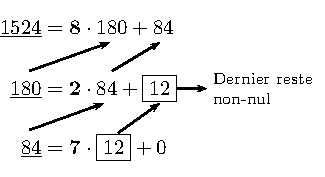
\includegraphics[scale=1]{Chapitre_2_arithmetique/figures/Correction/fig_co_1/fig_co_1.pdf}
\end{minipage}


On obtient $a=1524$ et $b=180$.




%14
\item
\begin{enumerate}[label=\alph*),itemsep=4mm]
\item 
Calculons $\pgdc(9945;3003)$ :

\hspace{6cm}\begin{minipage}[t][][b]{0.5\textwidth}
\vspace{-11.5mm}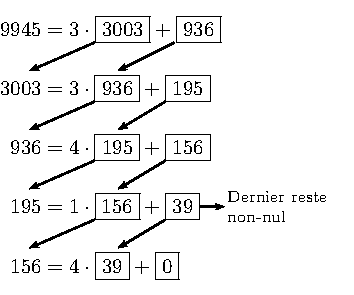
\includegraphics[scale=1]{Chapitre_2_arithmetique/figures/Correction/fig_co_2/fig_co_2.pdf}
\end{minipage}

\smallskip
Donc $\pgdc(9945;3003)=39$
\item 
$\pgdc(18480;9828)=84$
\item Par propriété du $\text{pgcd}$, pour tout entier $a$, $\text{pgcd}(-a; b) = \text{pgcd}(a; b)$.  

On a donc $\text{pgcd}(-286; 390) = \text{pgcd}(286; 390)$.

On effectue les divisions euclidiennes successives :
\begin{align*}
	390 &= 286 \cdot 1 + 104 \\
	286 &= 104 \cdot 2 + 78 \\
	104 &= 78 \cdot 1 + 26 \\
	78 &= 26 \cdot 3 + 0
\end{align*}

Le dernier reste non nul est $26$.  
Ainsi, $\text{pgcd}(-286; 390) = 26$.
\end{enumerate}


%EXERCICE
\item
\begin{itemize}\item[1)] Non car $\operatorname{PGCD}(4847 ; 5633)=131$
	
	$$
	\begin{aligned}
		5633 & =4847 \cdot 1+786 \\
		4847 & =786 \cdot 6+131 \\
		786 & =131 \cdot 6
	\end{aligned}
	$$
	
	\item[2)] Oui car $\operatorname{PGCD}(5617 ; 813)=1$
	
	$$
	\begin{aligned}
		5617 & =813 \cdot 6+739 \\
		813 & =739 \cdot 1+74 \\
		739 & =74 \cdot 9+73 \\
		74 & =73 \cdot 1+1
	\end{aligned}
	$$
\end{itemize}


%EXERCICE
\item $324=12 \cdot 27=12 \cdot 3^3$
$n$ doit être un multiple de 12 , mais pas un multiple de 36 sinon le $\operatorname{PGCD}(n ; 324)$ serait supérieur ou égal à 36 . Les entiers $n$ appartiennent à l'ensemble :
$\{12 ; 24 ; 48 ; 60 ; 84 ; 96 ; 120 ; 132 ; 156 ; 168 ; 192\}$.


%EXERCICE
\item On cherche le diviseur $b>9$ tel que :

$$
\left\{\begin{array} { l } 
	{ 1 8 0 9 = b q + 9 } \\
	{ 2 5 2 7 = b q ^ { \prime } + 7 }
\end{array} \Leftrightarrow \left\{\begin{array}{l}
	1800=b q \\
	2520=b q^{\prime}
\end{array} \Leftrightarrow\right.\right.
$$

$b>9$ et divise $\operatorname{PGCD}(4284 ; 3510)=360$
Le plus grand diviseur $b$ possible est donc 360 .



%15
\item\label{exer:pgdc_et_produit}
On note $(a;b)$ les couples de nombre entier de pgcd 14 et tels que $ab=7056$. Alors :
\begin{center}
$\left.\begin{tabular}{r}
$a=14\cdot a'$\\
$b=14\cdot b'$
\end{tabular}\right\rbrace$ avec $a'$ et $b'$ premiers entre eux.\end{center}
Comme $a\cdot b=7056$ alors $a'\cdot b'=\frac{7056}{14\cdot 14}=36$.

\medskip
Les possibilités pour $a'$ et $b'$ sont donc:
$$\boxed{\pt{1}{36}} \pvirg{4} \xcancel{\pt{2}{18}} \pvirg{4} \xcancel{\pt{3}{12}} \pvirg{4} \boxed{\pt{4}{9}} \pvirg{4} \xcancel{\pt{6}{6}}$$

Les couples qui ne sont pas premiers entre-eux ont étés barrés. Il reste donc 2 possibilités :
\renewcommand{\arraystretch}{1.4}
$$\begin{array}{r c l}
\pt{1}{36}& \overset{\cdot 14}{\longrightarrow} & \pt{14}{504} \\
\pt{4}{9} & \overset{\cdot 14}{\longrightarrow}  & \pt{56}{126}
\end{array}$$
Il y a alors deux couples vérifiant les conditions : $\pt{14}{504}$ et $\pt{56}{126}$.



%16
\item 
\begin{multicols}{2}
	\begin{enumerate}[label=\roman*),itemsep=5mm,left=-1mm,labelsep*=2mm]
		\item $3412=4\cdot 853+0$\\
		Donc $3412\equiv 0 \pmod{4}$
		\item $177=9\cdot 19+6$\\
		Donc $177\equiv 6 \pmod{9}$
		\item $31=31\cdot 1+0$\\
		Donc $31\equiv 0 \pmod{31}$
		\item $31=25\cdot 1+6$\\
		Donc $31\equiv 6 \pmod{25}$
		\item $365=5\cdot 73+0$\\
		Donc $365\equiv 0 \pmod{5}$
		\item $-3122=3\cdot (-1041)+1$\\
		Donc $-3122\equiv 1 \pmod{3}$
		\item $\nombre{31458687312}=10\cdot 3145868731+2$\\
		Donc $\nombre{31458687312}\equiv 2 \pmod{10}$
		\item $\nombre{-259874629}=10\cdot (-25987463)+1$\\
		Donc $\nombre{-259874629}\equiv 1 \pmod{10}$
	\end{enumerate}
\end{multicols}

%17
\item 
\begin{enumerate}[label=\roman*),itemsep=5mm,left=-1mm,labelsep*=2mm]
	\item[\textbf{a)}] \textbf{Vrai.} \\
	\textit{Justification :} $471 - 11 = 460$. Or $460 = 23 \cdot 20$, ce qui signifie que $23 \mid (471 - 11)$.
	
	\item[\textbf{b)}] \textbf{Faux.} \\
	\textit{Justification :} $370 - 17 = 353$. Or $353 = 13 \cdot 27 + 2$, donc $13 \nmid (370 - 17)$. \\
	(\textit{Autre méthode :} $370 = 13 \cdot 28 + 6 \implies 370 \equiv 6 \pmod {13}$ et $17 = 13 \cdot 1 + 4 \implies 17 \equiv 4 \pmod {13}$. Comme $6 \neq 4$, l'affirmation est fausse).
	
	\item[\textbf{c)}] \textbf{Vrai.} \\
	\textit{Justification :} $29 - (-121) = 29 + 121 = 150$. Or $150 = 5 \cdot 30$, donc $5 \mid (29 - (-121))$.
	
	\item[\textbf{d)}] \textbf{Faux.} \\
	\textit{Justification :} $-30 - (-1) = -30 + 1 = -29$. Or $-29$ n'est pas un multiple de $26$.
	
	\item[\textbf{e)}] \textbf{Vrai.} \\
	\textit{Justification :} Par définition de la congruence :
	\begin{itemize}
		\item $914 - 21 = 19 \cdot 47$, donc $19 \mid (914 - 21)$, d'où $914 \equiv 21 \pmod {19}$.
		\item De même, $47 \mid (914 - 21)$, d'où $914 \equiv 21 \pmod {47}$.
	\end{itemize}
	\textit{Remarque :} Bien que $21 \ge 19$ (ce n'est donc pas le reste de la division euclidienne par 19), l'égalité de congruence reste tout à fait exacte.
	
	\item[\textbf{f)}] \textbf{Vrai.} \\
	\textit{Justification :} Par définition, $b \equiv 0 \pmod a \iff b - 0 = k \cdot a \iff b = k \cdot a \iff a \mid b$.
	
	\item[\textbf{g)}] \textbf{Vrai.} \\
	\textit{Justification :} Si $b \equiv 0 \pmod a$ et $c \equiv 0 \pmod a$, alors $a \mid b$ et $a \mid c$. Par propriété de la divisibilité, $a$ divise toute combinaison linéaire $\alpha b + \beta c$ pour tous entiers $\alpha, \beta$, d'où $\alpha b + \beta c \equiv 0 \pmod a$.
\end{enumerate}

\item

\begin{itemize}
	\item \textbf{Étude de $351$ :}
	$$351 = 7 \cdot 50 + 1 \implies 351 \equiv 1 \pmod 7$$
	Par compatibilité avec les puissances :
	$$351^{12} \equiv 1^{12} \equiv 1 \pmod 7$$
	
	\item \textbf{Étude de $85$ :}
	$$85 = 7 \cdot 12 + 1 \implies 85 \equiv 1 \pmod 7$$
	Par compatibilité avec les puissances :
	$$85^{15} \equiv 1^{15} \equiv 1 \pmod 7$$
	
	\item \textbf{Produit :}
	Par compatibilité avec la multiplication :
	$$351^{12} \cdot 85^{15} \equiv 1 \cdot 1 \equiv 1 \pmod 7$$
\end{itemize}



% exo
\item

\begin{enumerate}
	\item \textbf{Étude du premier terme $5^{2n}$ :}
	On réécrit la puissance à l'aide des règles de calcul :
	$$5^{2n} = \left(5^2\right)^n = 25^n$$
	
	Or, $25 = 11 \cdot 2 + 3$, donc :
	$$25 \equiv 3 \pmod{11}$$
	
	Par compatibilité de la congruence avec les puissances, on a :
	$$5^{2n} \equiv 3^n \pmod{11}$$
	
	\item \textbf{Étude du second terme $14^n$ :}
	On effectue la division euclidienne de $14$ par $11$ :
	$$14 = 11 \cdot 1 + 3 \implies 14 \equiv 3 \pmod{11}$$
	
	Par compatibilité de la congruence avec les puissances, on a :
	$$14^n \equiv 3^n \pmod{11}$$
	
	\item \textbf{Soustraction des congruences :}
	Par compatibilité avec la soustraction :
	$$5^{2n} - 14^n \equiv 3^n - 3^n \pmod{11}$$
	$$5^{2n} - 14^n \equiv 0 \pmod{11}$$
\end{enumerate}

\textbf{Conclusion :} 
Pour tout entier naturel $n$, $5^{2n} - 14^n$ est divisible par $11$.


%17
\item
\begin{enumerate}[label=\roman*),itemsep=5mm,left=-1mm,labelsep*=2mm]
	\item $\phantom{195}1=13\cdot 0+1$\\
	$1951=13\cdot 150+1$\\
	$1964=13\cdot 151+1$\\
	$1977=13\cdot 152+1$\\
	$1990=13\cdot 153+1$ \eh{4} Donc, $1\equiv 1951 \equiv 1964 \equiv 1977 \equiv 1990 \pmod{13}$
	
	\item $1776=40\cdot 44+16$\\
	$1976=40\cdot 49+16$ \eh{4} Donc, $16\equiv 1776 \equiv 1976  \pmod{40}$
	
	\item $1929=15\cdot 128+9$\\
	$1959=15\cdot 130+9$\\
	$1974=15\cdot 131+9$\\
	$1989=15\cdot 132+9$ \eh{4} Donc, $9\equiv 1929 \equiv 1959 \equiv 1974 \equiv 1989 \pmod{15}$
	
\end{enumerate}




%18
\item 
\begin{enumerate}[label=\arabic*),itemsep=3mm,left=-1mm,labelsep*=2mm]
	\item On vérifie la véracité de la proposition pour $n=0$ et $n=1$ :
	
	\smallskip
	$6\cdot 4^0=6=9\cdot 0 +6$ donc $6\cdot 4^0\equiv 6 \pmod{9}$
	
	\smallskip
	$6\cdot 4^1=24=9\cdot 2 +6$ donc $6\cdot 4^1\equiv 6 \pmod{9}$
	
	\item Supposons que $6\cdot 4^n\equiv 6 \pmod{9}$ pour un certain $n\in \N$ et montrons que la proposition est vraie pour $n+1$.
	
	\smallskip
	Comme $6\cdot 4^n\equiv 6 \pmod{9}$, par définition cela signifie que $\exists k\in \Z$ tel que $6\cdot 4^n=6+9k$. On a alors :
	$$6\cdot 4^{n+1}=6\cdot 4^n\cdot 4=(6+9k)\cdot 4=24+36k=6+18+36k=6+9(2+4k)$$
	
	On pose $k'=2+4k$ et on obtient $6\cdot 4^{n+1}=6+9k'$.
	
	\smallskip
	On conclut alors que $6\cdot 4^{n+1} \equiv 6 \pmod{9}$
\end{enumerate}
\clearpage



%19
\item
Il s'agit de calculer $100^{1000}$ modulo $13$. 

\smallskip
Tout d'abord remarquons que $100 \equiv 9 \pmod{13}$ donc  $100^{1000} \equiv 9^{1000} \pmod{13}$. 

\smallskip
Puis, plusieurs raisonnements sont possibles. En voici deux :

\begin{enumerate}[label=\roman*)]
	\item $9^{2} \equiv 81 \equiv 3 \pmod{13}$ et donc $9^{3} \equiv 9^2\cdot 9 \equiv 3\cdot 9 \equiv 1 \pmod{13}$
	
	On conclut avec: $$100^{1000} \equiv 9^{1000} \equiv 9^{3\cdot 333+1} \equiv \left(9^3\right)^{333}\cdot9  \equiv 1^{333}\cdot9 \equiv 9 \pmod{13}$$
	
	\item $9^{2} \equiv 81 \equiv 3 \pmod{13}$ et donc $9^{5} \equiv \left(9^2\right)^2\cdot 9 \equiv 3^2\cdot 9 \equiv 81 \equiv 3 \pmod{13}$.
	
	On déduit que $9^{10} \equiv \left(9^5\right)^2 \equiv 3^2 \equiv  9 \pmod{13}$
	
	On conclut avec : $$100^{1000} \equiv 9^{1000} \equiv \left(\left(9^{10}\right)^{10}\right)^{10} \equiv \left(9^{10}\right)^{10}  \equiv 9^{10} \equiv 9 \pmod{13}$$
\end{enumerate}




%20
\item
Raisonnons modulo $8$ et remarquons que $7 \equiv -1 \pmod{8}.$

\smallskip
D'où on tire :
$$7^n +1 \equiv (-1)^n + 1 \pmod{8}.$$

Le reste de la division euclidienne de $7^n+1$ par $8$ est $r(n)=(-1)^n+1$.

\begin{itemize}
	\item Si $n$ est impair alors $r(n)=(-1)^n+1=0$ et $7^n+1$ est divisible par $8$.
	
	\item Si $n$ est pair alors $r(n)=(-1)^n+1=2$ et $7^n+1$ n'est pas divisible par $8$ (et le reste vaut $2$).
\end{itemize}




%21
\item
\begin{enumerate}[label=\alph*),itemsep=5mm,left=-1mm,labelsep*=2mm]
	\item $12 \equiv 1 \pmod{11} \Rightarrow 12^{15} \equiv 1 \pmod{11}$.
	
	\ev
	Le reste de la division de $12^{15}$ par 11 est 1.
	\item $10 \equiv -1 \pmod{11} \Rightarrow 10^{7} \equiv -1 \equiv 10 \pmod{11}$.
	
	\ev
	Le reste de la division de $10^{7}$ par 11 est 10.
	\item $78 \equiv 1 \pmod{11} \Rightarrow 78^{15} \equiv 1 \pmod{11}$.
	
	\ev
	Le reste de la division de $78^{15}$ par 11 est 1.
	\item $13 \equiv 2 \pmod{11} \Rightarrow 13^{12} \equiv 2^{12} \pmod{11}$.
	
	\ev
	Nous avons $2^4=16 \equiv 5 \pmod{11} \Rightarrow \left(2^4\right)^3 \equiv 125 \equiv 4 \pmod{11}$.
	
	\ev
	Le reste de la division de $13^{12}$ par 11 est 4.
	\item $\left(-2\right)^6 = 64 \equiv -2 \pmod{11}$.
	
	\ev
	Nous avons $\left(-2\right)^{19} = \left(\left(-2\right)^6\right)^3\cdot(-2) \equiv \left(-2\right)^3\cdot(-2) \equiv 16 \equiv 5 \pmod{11}$.
	
	\ev
	Le reste de la division de $\left(-2\right)^{19}$ par 11 est 5.
\end{enumerate}




%22
\item
\begin{enumerate}[label=\alph*),itemsep=5mm,left=-1mm,labelsep*=2mm]
	\item \begin{itemize}\setlength{\itemsep}{2mm}
		\item $2^4=17\cdot 1 -1  \eh{1}\Rightarrow\eh{1} 2^4\equiv -1 \pmod{17}$.
		\item $6^2=17\cdot 2 +2  \eh{1}\Rightarrow\eh{1} 6^2\equiv 2 \pmod{17}$.
	\end{itemize}
	
	\item \begin{itemize}\setlength{\itemsep}{2mm}
		\item On a $1532=90\cdot 17 +2$. Donc $[1532]_{17}=[2]_{17}$
		\item On a $346=20\cdot 17 +6$. Donc : $[346]_{17}=[6]_{17}$ 
	\end{itemize}
	
	\item \begin{itemize}\setlength{\itemsep}{2mm}
		\item $1532^{20}\equiv 2^{20} \equiv\left(2^4\right)^5 \equiv (-1)^5 \equiv -1 \equiv 16 \pmod{17}.$
		
		\smallskip
		Le reste de la division de $1532^{20}$ par 17 est 16.
		\item $346^{12}\equiv 6^{12} \equiv\left(6^2\right)^6 \equiv 2^6 \equiv 2^4\cdot 4 \equiv -4 \equiv 13 \pmod{17}.$
		
		\smallskip
		Le reste de la division de $346^{12}$ par 17 est 13.
	\end{itemize}
\end{enumerate}




%23
\item
\begin{multicols}{3}
	\begin{enumerate}[label=\alph*)]
		\item $S= \lbrace \left[6\right]_7\rbrace$
		\item $S= \lbrace \left[11\right]_{30} \; ; \; \left[26\right]_{30} \rbrace$
		\item[]
	\end{enumerate}
\end{multicols}




%24
\item
\begin{enumerate}[label=\alph*),itemsep=7mm,left=-1mm,labelsep*=2mm]
	\item\label{a} Soit $n$ un nombre impair, alors il s'écrit $n=2k+1$ avec $k\in \Z$. Alors :
	
	$$n^2 = (2k+1)^2 = 4k^2+4k+1 = 4k(k+1) + 1.$$ Par ailleurs, de $k$ ou $k+1$ l'un des deux est pair, donc $4k(k+1)$ est un multiple de 8.
	
	Donc $n^2 \equiv 1 \pmod{8}$ et le reste de la division de $n^2$ par $8$ est $1$.
	
	\item\label{b} Si $n$ est pair alors il existe $k\in \Z$ tel que $n=2k$ et $n^2 = 4k^2$.
	
	\begin{itemize}
		\item Si $k$ est pair alors il existe $j\in \Z$ tel que $k=2j$ et $k^2=4j^2$.
		
		Donc $n^2 = 4k^2 = 16j^2$ est divisible par $8$. Finalement $n^2 \equiv 0 \pmod{8}$.
		
		\item Si $k$ est impair alors il existe $j\in \Z$ tel que $k=2j+1$ et $k^2=4j^2+4j+1$.
		
		Donc $n^2 = 4k^2=16(j^2+j)+4$ est divisible par 4 mais pas par 8.
		
		Finalement $n^2 \equiv 4 \pmod{8}$. 
	\end{itemize}
	
	\item\label{c} \begin{itemize}\setlength{\itemsep}{4mm}
		\item Comme $a, b, c$ sont impairs alors d'après la question \ref{a} on a :
		
		\medskip
		\centerline{$a^2 \equiv 1 \pmod{8}$\ehh,\ehh $b^2 \equiv 1 \pmod{8}$\ehh,\ehh$c^2 \equiv 1 \pmod{8}$.}
		
		\medskip
		Donc $a^2+b^2+c^2 \equiv 1+1+1 \equiv 3 \pmod{8}$.
		
		\item On écrit $a = 2k+1$, $b=2j+1$ et $c=2i+1$, alors :
		$$2ab = 2(2k+1)(2j+1) = 8kj + 4(k+j)+2$$
		$$2bc = 2(2j+1)(2i+1) = 8ji + 4(j+i)+2$$
		$$2ac = 2(2k+1)(2i+1) = 8ki + 4(k+i)+2$$
		Donc :
		$$2(ab+bc+ca)= 8kj+8ji+8ki + 8(k+j+i)+6= 8(kj+ji+ki+k+j+i)+6$$
		Finalement $2(ab+bc+ca) \equiv 6 \pmod{8}$.
	\end{itemize}
	
	\item \begin{enumerate}[label=\roman*)] 
		\item Montrons par l'absurde que le nombre $a^2+b^2+c^2$ n'est pas le carré d'un nombre entier.
		
		\smallskip
		Supposons qu'il existe $n\in \N$ tel que $a^2+b^2+c^2=n^2$. 
		
		\smallskip
		D'une part, nous avons montré au point \ref{c} que $a^2+b^2+c^2 \equiv 3 \pmod{8}$.
		
		\smallskip
		D'autre part, nous avons montré au point \ref{b} que si $n$ est impair alors $n^2 \equiv 1 \pmod{8}$ et si $n$ est pair alors
		$n^2 \equiv 0 \pmod{8}$ ou $n^2 \equiv 4 \pmod{8}$.
		
		\smallskip
		Dans tous les cas $n^2$ n'est pas congru à $3$ modulo $8$. Donc il y a une contradiction et nous concluons que $a^2+b^2+c^2$ n'est pas un carré.
		
		\item On fait le même raisonnement avec $2(ab+bc+ca)$.
		
		\item Pour $ab+bc+ca$ l'argument est similaire : 
		d'une part $2(ab+bc+ca)\equiv 6 \pmod{8}$
		et d'autre part si, par l'absurde, on suppose $ab+bc+ca=n^2$ alors
		selon la parit\'e de $n$ nous avons $2(ab+bc+ca)\equiv 2n^2 \equiv 2 \pmod{8}$
		ou \`a $0 \pmod{8}$. Dans les deux cas cela aboutit à une contradiction. On conclut que
		$ab+bc+ca$ n'est pas un carré.
	\end{enumerate}
\end{enumerate}




%16
\item
\begin{enumerate}[label=\alph*),itemsep=4mm]
\item
En effectuant la remontée de l'algorithme d'Euclide on obtient:
$$\pgdc(7260;637)=1=\bm{(141)}\cdot 7260 + \bm{(-1607)}\cdot 637$$
\item
En effectuant la remontée de l'algorithme d'Euclide on obtient:
$$\pgdc(9945;3003)=39=\bm{(-16)}\cdot 9945 + \bm{(53)}\cdot 3003$$
\end{enumerate}





%17
\item
On utilise le corolaire 2.6 et on pose $u=-1$ et $v=1$ : $(-1)\fois a+1\fois(a+1)=1$. Donc $\pgdc(a;a+1)=1$.




\clearpage
%18
\item
\begin{enumerate}[label=\alph*),itemsep=1mm]
\item $x=241 \et{2} y=-364$. \eh{2} On obtient $873\fois \bm{241}+578\fois \bm{(-364)}=1$
\item $x=-345 \et{2} y=190$ \eh{2} On obtient $315\fois \bm{(-345)}+572\fois \bm{(190)}=5$
\item Cette équation n'a pas de solution dans $\Z^2$. {\small(La somme ou la différence de deux nombres paires sera toujours paire)}
\end{enumerate}




%19
\item
Il faut utiliser le fait que\eh{1} $\pgdc(a;b)\fois \ppmc(a;b)=\vert ab\vert$. On déduit que $\vert ab\vert=5184$.

\smallskip
On fait le même raisonnement qu'à l'exercice \ref*{exer:pgdc_et_produit} et on trouve: $\pt{\pm 12}{\pm 432}$ et $\pt{\pm 48}{\pm 108}$ {\small (soit $8$ couples)}. 



%20
\item



%21
\item




%22
\item \begin{minipage}[t][][b]{1\textwidth}
\insertcode{Chapitre_2_arithmetique/Programmes/Eratosthene.py}{0.9}{}
\end{minipage}




%23
\item
Par exemple $5x-2y=-24$.

\smallskip
Il suffit de choisir aléatoirement $a,b \in \N$ puis de calculer $c\in \N$ tel que $a\cdot 24+b\cdot 72=c$.




%24
\item
\begin{enumerate}[label=\alph*),itemsep=5mm,left=-1mm,labelsep*=2mm]
\vspace{-3mm}
\item Il faut résoudre le système d'équations suivant dans $\Z$:
$\left\lbrace\begin{array}{@{\eh{1}}r@{\eh{1}}c@{\eh{1}}c@{\eh{1}}c@{\eh{1}}l}
6a   & + & 17b & = & c\\
-18a & - & 23b & = & c\\
\end{array}\right.$

S'agissant d'un système sous-déterminé, il possède une infinité de solutions toutes de la forme :
$$\left(-\frac{5}{21}\alpha\; ;\; \frac{1}{7}\alpha \; ;\; \alpha \right)$$

Pour que les solutions soient entières, il faut que $\alpha$ soit un multiple de ppmc$(7,21)=21$. 

\smallskip
Finalement nous obtenons : $S=\lbrace \left(-5\beta\; ;\; 3\beta \; ;\; 21\beta \right) \mid \beta\in \Z \rbrace$

\smallskip
On conclut que toute équation de la forme $-5\beta\cdot x+ 3\beta\cdot y = 21\beta$ avec $\beta\in \Z$ est une équation diophantienne ayant $(6;17)$ et $(-18;-23)$ pour solutions.

\item Comme nous venons de le voir, il existe une infinité d'équations ayant pour solutions $(6;17)$ et $(-18;-23)$, cependant ces équations sont toutes équivalentes. On peut remarquer que les solutions d'une équation du type $ax+by=c$ forment une droite. Par deux points passant une et une seule droite (1er axiome d'Euclide), l'équation cherchée est donc celle d'une droite, qui peut être donnée par une infinité d'équations mais toutes équivalentes. 
\end{enumerate}




%25
\item 
Grâce à l'algorithme d'Euclide nous trouvons que pgcd$(1665;1035)=45$. Comme $45\ | \ 45$, la proposition 2.14 assure que cette équation possède des solutions. La remontée de l'algorithme fourni une solution particulière à l'équation (les coefficients de Bézout) : 
$$1665\cdot \bm{5} + 1035 \cdot \bm{(-8)} = 45$$
Une solution particulière de $(E)$ est donc $(x_0,y_0) = (5,-8)$.

%\medskip
%Nous allons maintenant trouver l'expression générale pour les solutions de l'équation $(E)$.

\medskip
Soit alors $(x,y)$ une solution quelconque de l'équation $1665x+1035y=45$. Comme $(x_0,y_0)$ est aussi solution, nous avons $1665x_0+1035y_0=45$. En faisant la différence de ces deux égalités nous obtenons :

$$1665(x-x_0)+1035(y-y_0)=0 \quad\ssi$$
$$1665(x-x_0)=-1035(y-y_0) \quad\overset{:45}{\ssi}$$
$$37(x-x_0)=-23(y-y_0) \quad (*)$$

\medskip
On en déduit que $37\ |\ -23 (y-y_0)$ et comme pgcd$(37;23)=1$ le lemme de Gauss assure que
$37\ |\ (y -y_0)$ (c'est ici qu'il est important d'avoir divisé par $45$!).

\medskip
Cela nous permet d'écrire $y-y_0 = 37 k$ pour un $k \in \Z$. Repartant de l'égalité $(*)$ nous obtenons alors  : $37(x-x_0)=-23 \cdot 37 \cdot k$.
Ce qui donne $x-x_0 = -23 k$.

\medskip
Donc si $(x,y)$ est solution de $(E)$ alors elle est de la forme :
$(x,y)= (x_0 - 23k,y_0+37k)$, avec $k \in \Z$.

Réciproquement pour chaque  $k\in\Z$, si $(x,y)$ est de cette forme alors c'est une solution de $(E)$
(vérifiez-le !).\\
Finalement  :
$$S=\big\lbrace (5 - 23k,-8+37k) \mid k\in \Z\big\rbrace.$$



%26
\item
L'algorithme d'Euclide donne pgcd$(35;84)=7$.
%\begin{align*}
%84 & =35\cdot 2 +14\\
%35 & = 14\cdot 2 +7\\
%14 & =7\cdot 2 +0
%\end{align*}

\medskip
Attendu que $7$ ne divise pas $150$, l'équation diophantienne $35x+84y=150$ n'admet pas de solution entière. La droite d'équation $35x+84y=150$ ne passe donc par aucun point à coordonnées entières et ne croise donc jamais une intersection du quadrillage.
%pour déterminer le pgcd de $35$ et $84$ donne :




%27
\item
\begin{enumerate}[label=\alph*),itemsep=5mm,left=-1mm,labelsep*=2mm]
\item Soit : \begin{minipage}[t]{0.9\textwidth}
$\boldsymbol{x} :$ le nombre d'étudiants ayant participé au repas.

\smallskip
$\boldsymbol{y} :$ le nombre d'enfants ayant participé au repas.

\smallskip
$\boldsymbol{28-x-y} :$ le nombre d'adultes ayant participé au repas.
\end{minipage}

\smallskip
Le problème se traduit donc par l'équation diophantienne :\vspace{-1mm}
$$17x+13y+26(28-x-y)=613 \ehhh \ssi \ehhh \boldsymbol{9x+13y=115} \ehh \textrm{(E)}$$

\item Le couple $(3\; ;-2)$ est une solution évidente de $9x+13y=1$, donc :
$$\left(115\cdot 3\; ; 115\cdot (-2)\right)=(345\;-230)$$ est une solution particulière de (E).
En soustrayant la solution particulière de la solution générale, on trouve :
$$9(x-345)=13(-230-y)$$
Comme pgcd$(13\; ; 9)=1$, on en déduit, d'après le lemme de Gauss, que $13$ divise $x-345$ et que $9$ divise $(-230-y)$. On trouve alors :
\renewcommand{\arraystretch}{1.3}
$$\left\lbrace\begin{array}{l}
x=13k+345\\
y=-9k-230
\end{array}\right. \textrm{avec } k\in \Z$$
Comme $x$ et $y$ sont des nombres positifs, on a :
$$\left\lbrace\begin{array}{l}
13k+345\geqslant 0\\
-9k-230 \geqslant 0
\end{array}\right. \ehhh \ssi \ehhh \renewcommand{\arraystretch}{2.2}%%%%%%%%%%%%%%%%%%%
\left\lbrace\begin{array}{l}
k\geqslant -\frac{345}{13}\simeq -26,5\\
k \leqslant -\frac{230}{9}\simeq -25,6
\end{array}\right.$$
La seule valeur possible est alors $k=-26$ et on trouve $x=7$ et $y=4$.

\smallskip
Il y a donc 7 étudiants, 4 enfants et 17 adultes.
\item  ~

\vspace{-5mm}
\begin{center}
\comp{\fbox{\begin{minipage}[t]{0.72\textwidth}\setlength{\arrayrulewidth}{2pt}

\textbf{Variable :} $x$, $y$ (entiers)\\
\textbf{Début}

\vspace{2mm}
\begin{tabular}{|c}
\begin{minipage}{\textwidth}
	\textbf{Pour} $x$ de 0 à 28 \textbf{Faire}\vspace{2mm}\\
	\begin{tabular}{|c}
	\begin{minipage}{\textwidth}
			\textbf{Pour} $y$ de 0 à 28 \textbf{Faire}\vspace{2mm}\\
			\begin{tabular}{|c}\vspace{2mm}
			\begin{minipage}{\textwidth}
					\textbf{Si} $9x+13y=115$ \textbf{Alors}\\
					\begin{tabular}{|c}
					\begin{minipage}{\textwidth}
						\textbf{Afficher} "Il y a " x " étudiants et " y " enfants."
					\end{minipage}
					\end{tabular}\vspace{1mm}\\
					\textbf{FinSi}
			\end{minipage}
			\end{tabular}\vspace{1mm}\\
			\textbf{FinPour}
	\end{minipage}
	\end{tabular}\vspace{3mm}\\
	\textbf{FinPour}
\end{minipage}
\end{tabular}

\vspace{2mm}
{\bf Fin}
\end{minipage}}}
\end{center}
\end{enumerate}












\end{enumerate}





















%\end{multicols*}
\fontsize{11}{12}\selectfont



%\setcounter{chapter}{1}
%\chapter{Analyse Numérique}
%\renewcommand{\titrechapitre}{Analyse Numérique}
%\thispagestyle{fancy}
%\colorlet{couleurchapitre}{green!30!black}
%\setcounter{compteurexo}{1}
%\setcounter{compteuremarque}{1}
%\setcounter{page}{45}
%
%\vspace{-1cm}
\setcounter{section}{-1}
\section{Introduction}
L'analyse numérique est un vaste champ d'étude des mathématiques qui a pour objectif de fournir des solutions approchées à des problèmes concrets. On cherche à mettre en place des méthodes numériques -souvent algorithmiques- qui permettent d'approximer le résultat de certains problèmes.%, parmi lesquels ont peut citer l'évaluation d'une fonction en un point, la résolution d'équations et de système d'équations, le calcul d'une intégrale\footnote{Le concept \guillemets{d'intégrales} sera présenté en cours de mathématique de 4\up{ème} année.}, l'interpolation\footnote{\guillemets{L'interpolation} tente de retrouver l'expression algébrique d'une fonction passant par des points donnés.} ou encore l'optimisation.


\medskip Les équations sont des objets que l'on rencontre fréquemment en mathématiques et l'intérêt pour leur résolution apparaît dans de nombreux contextes scientifiques. Dans la passé, la résolution numérique d'équations a été un moteur pour le développement de plusieurs notions  mathématiques et c'est probablement un des domaines les plus anciens de l'analyse numérique.

\medskip La plupart des phénomènes physiques, chimiques ou biologiques issus de la technologie moderne sont régis par des équations complexes. C'est en étudiant et en observant la nature de ces phénomènes que nous parvenons à modéliser leur fonctionnement à l'aide d'outils mathématiques. Cependant, la recherche de solutions à ces équations peut être (et est très souvent!) compliquée car la modélisation fait intervenir beaucoup de paramètres.


\medskip Le développement, relativement récent, de puissants moyens de calculs a ouvert de nouvelles pistes d'explorations ainsi que de nouvelles perspectives de recherches pour répondre aux besoins de l'ingénierie. Cette dernière a besoin de méthodes efficaces pour résoudre des équations et  la résolution numérique de ces équations à l'aide d'un ordinateur nécessite des connaissances approfondies en mathématiques.

\medskip
Nous allons étudier trois méthodes permettant de résoudre numériquement des équations.

%Nous le travaillons activement en mathématiques mais la recherche d'une quantité manquante est un questions récurrente dans  toutes les autres sciences (au sens large).

%\medskip Nombre de phénomènes physiques, chimiques, économiques, sociaux, démographiques, naturels, et la liste est encore longue, sont modélisés à l'aide d'équations qui permettent de décrire non seulement la nature du phénomène mais également de répondre à certaines questions et résoudre des problèmes.  


%
\section{La méthode de la dichotomie}

%---------------------------------------------------------------
\subsection{Principe de la dichotomie}

Le principe de la dichotomie\footnote{Du grec \foreignlanguage{greek}{dikotomia} qui signifie \guillemets{partager en deux}.} repose sur la version suivante du théorème des valeurs intermédiaires :

\begin{theoreme}[\small \textit{théorème des valeurs intermédiaires}]\label{thm_valeurs_intermediaires}
Soit $f:[a,b]\to\R$ une fonction continue. Si $f(a)\fois f(b) \leqslant 0$, alors il existe $c\in[a,b]$ tel que $f(c)=0$.
\end{theoreme}

%La condition $f(a)\cdot f(b)\le0$ signifie que $f(a)$ et $f(b)$ sont de signes opposés (ou que l'un des deux est nul). L'hypothèse de continuité est essentielle !



\medskip


\begin{minipage}[t][][b]{0.6\textwidth}
En d'autres mots, si la fonction $f$ est continue et change de signe dans l'intervalle $[a,b]$, alors il existe au moins une solution à l'équation $f(x)=0$ dans l'intervalle $[a,b]$. 

\smallskip
Remarquons que toute équation $f(x)=g(x)$ peut être ramenée à la recherche d'un zéro de la fonction ${h(x)=f(x)-g(x)}$.

\medskip
Comme souvent en \guillemets{mathématique pure}, le théorème de la moyenne \textbf{n'est pas un théorème constructif}. C'est un \textbf{théorème d'existence} et il ne dit malheureusement pas comment déterminer le zéro de la fonction qui doit exister dans l'intervalle $[a;b]$.

\vspace{2mm}
\end{minipage}\hspace{2mm}\begin{minipage}[t][][b]{0.45\textwidth}
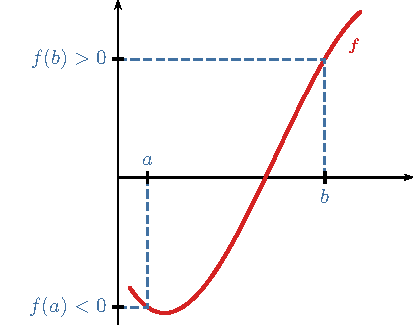
\includegraphics[scale=0.9]{Chapitre_3_analyse_numerique/figures/fig_1/fig_1.pdf}

\fig{Théorème de la valeur intermédiaire.}
\end{minipage}


La continuité ainsi que la condition $f(a)\cdot f(b)<0$ sont essentielles à l'existence d'un zéro dans l'intervalle $[a;b]$. Si l'une ou l'autre de ces hypothèses n'est pas satisfaite, le théorème de la valeur intermédiaire ne peu garantir l'existence d'un zéro dans l'intervalle $[a;b]$.

\vspace{5mm}
\begin{minipage}{0.48\textwidth}
\begin{center}
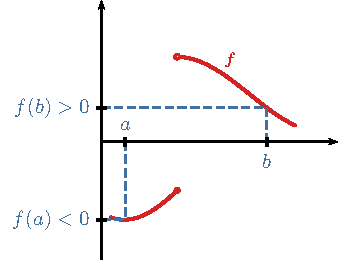
\includegraphics[scale=1]{Chapitre_3_analyse_numerique/figures/fig_2/fig_2.pdf}

\smallskip
\fig{La fonction $f$ n'est pas continue et elle n'admet pas de zéro dans l'intervalle $[a;b]$.}
%\textit{\small La fonction $f$ n'est pas continue et elle n'admet pas de zéro dans l'intervalle $[a;b]$ }
\end{center}
\end{minipage}\hspace{8mm}\begin{minipage}{0.47\textwidth}
\begin{center}
\hspace{-5mm}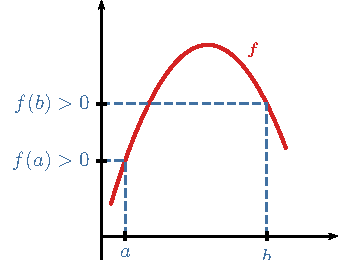
\includegraphics[scale=1]{Chapitre_3_analyse_numerique/figures/fig_3/fig_3.pdf}

\smallskip
\fig{La fonction $f$ ne vérifie pas $f(a)\cdot f(b)<0$ et elle n'admet pas de zéro dans l'intervalle $[a;b]$.}
%\textit{\small La fonction $f$ ne vérifie pas $f(a)\cdot f(b)<0$ et elle n'admet pas de zéro dans l'intervalle $[a;b]$ }
\end{center}
\end{minipage}



\vspace{6mm}
La dichotomie consiste à diviser l'intervalle $[a;b]$ en son milieu puis à \guillemets{détecter} de quel côté du point milieu se situe le zéro. En poursuivant le procédé avec les intervalles suivants, obtenus par répétition de l'opération, on obtient une suite d'intervalles \guillemets{emboités} dont la longueur tend vers 0 et dont les extrémités des intervalles forment 2 suites convergentes vers un zéro de la fonction.


\medskip
Le principe est la suivant : soit $f : [a,b] \to \R$ une fonction continue et telle que $f(a)\cdot f(b)\leqslant 0$.
%\end{minipage}





\begin{itemize}
  \item Si $f(a)\cdot f(\frac{a+b}{2})\le0$, alors il existe
  $c \in [a,\frac{a+b}{2}]$ tel que $f(c)=0$.
  \item Si $f(a)\cdot f(\frac{a+b}{2})>0$ alors
  $f(\frac{a+b}{2})\cdot f(b)\le0$ et donc il existe $c \in [\frac{a+b}{2},b]$ tel que $f(c)=0$.
\end{itemize}


\begin{center}
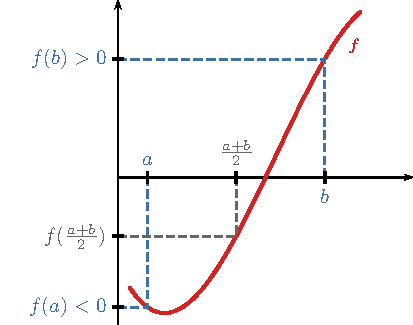
\includegraphics[scale=1]{Chapitre_3_analyse_numerique/figures/fig_4/fig_4.pdf}

\fig{Le zéro se trouve dans la partie droite de l'intervalle $[a;b]$.}
\end{center}


Le nouvel intervalle obtenu contient une solution de l'équation $f(x)=0$ et il a une longueur de moitié par rapport à l'intervalle précédent.


\subsubsection{Le processus algorithmique de la dichotomie}

\begin{itemize}
  \item[] \eh{4.2}{\bf Etape 0 :}\eh{4} On pose $a_0=a$, $b_0=b$. 
  \item[] \eh{4.2}{\bf Etape 1 :}\eh{3}\begin{minipage}[t]{0.8\textwidth}
    $\bullet$  Si $f(a_0)\cdot f(\frac{a_0+b_0}{2}) \le 0$, alors on pose $a_1=a_0$ et $b_1=\frac{a_0+b_0}{2}$,
    
    \smallskip
    $\bullet$ Sinon on pose $a_1=\frac{a_0+b_0}{2}$ et $b_1=b_0$.
 \end{minipage}

  %\item ...
  \item[] {\bf Etape $n+1$ :} \eh{3}\begin{minipage}[t]{0.8\textwidth}
   $\bullet$ Si $f(a_n)\cdot f(\frac{a_n+b_n}{2}) \le 0$, alors on
   pose $a_{n+1}=a_n$ et $b_{n+1}=\frac{a_n+b_n}{2}$,
   
   \smallskip
  $\bullet$ Sinon on pose $a_{n+1}=\frac{a_n+b_n}{2}$ et $b_{n+1}=b_n$.
 \end{minipage}

\end{itemize}

\subsubsection{Justification Mathématique}
L'algorithme décrit ci-dessus permet bien de localiser un zéro de la fonction $f$ prévu par le théorème de la moyenne. C'est ce que démontre le théorème suivant.

\smallskip
\begin{theoreme}[\small \textit{convergence dichotomique}]
Soit $f:[a,b]\to\R$ une fonction continue telle que $f(a)\cdot f(b) \leqslant 0$.\\
Soit également $[a_n;b_n]$ la suite d'intervalles obtenus par le processus dichotomique.

\smallskip
Alors $(a_n)_{n\geqslant 0}$ et $(b_n)_{n\geqslant 0}$ forment deux suites convergentes vers un zéro $c$ de la fonction $f$. 
\end{theoreme}

\smallskip


\begin{demonstration}

A chaque étape de l'algorithme, on obtient deux nombres $a_n$ et $b_n$ tels que :
$$a\leqslant a_{n} \leqslant a_{n+1} \leqslant b_{n+1}\leqslant  b_n \leqslant b$$

%On arrête le processus dès que $b_n-a_n=\frac{b-a}{2^n}$ est inférieur à la précision souhaitée.


Par construction, $(a_n)_{n\in \N}$ et $(b_n)_{n\in \N}$ sont deux suites bornées ainsi que croissante et décroissante respectivement. Donc les deux suites sont convergentes.

\medskip
Par ailleurs, toujours par construction, $(b_n-a_n)=\frac{b-a}{2^n} \to 0$ quand $n\to \infty$ et donc les suites $(a_n)_{n\in \Z}$ \et{1} $(b_n)_{n\in \Z}$ convergent vers la même valeur. 

\medskip
Vu que $a_n\leqslant c\leqslant b_n\eh{2} \forall n\in\N$, on a :
$$\lin{\infty} a_n\leqslant c\leqslant \lin{\infty} b_n$$

\medskip
et comme les suites convergent vers la même valeur alors par le \guillemets{théorème du sandwich}  :
$$\lin{\infty} a_n=c=\lin{\infty} b_n$$

\vspace{-3mm}
\hfill $\blacksquare$
\end{demonstration}




%---------------------------------------------------------------
\subsection{Applications : approximation de  $\sqrt{2}$}

Nous allons utiliser le processus dichotomique pour calculer une valeur approchée de $\sqrt{2}$. Il faut choisir judicieusement la fonction $f$ ainsi que le bornes $a$ et $b$ de l'intervalle.

\medskip
On choisit $f(x)=x^2-2$. C'est une fonction continue sur $\R$ qui s'annule en $\pm\sqrt{2}$ et $\sqrt{2}$ est l'unique solution positive de l'équation $f(x)=0$.

\medskip
Par ailleurs, $f(1) \leqslant 0$ et $f(2) \geqslant 0$, donc l'équation $f(x)=0$ admet une solution dans l'intervalle $[1,2]$. Cette solution est donc nécessairement $\sqrt{2}$.


%Notez que l'on ne choisit pas pour $f$ la fonction $x\mapsto x-\sqrt{2}$ car on ne connaît pas la valeur de $\sqrt{2}$. C'est ce que l'on cherche à calculer !




\begin{enumerate}[label=\arabic*)]
\item On pose $a_0=1$ \et{1} $b_0=2$ \eh{0.2} puis on calcule $\frac{1+2}{2} = 1,5$.
$$f(1,5)=0.25\geqslant 0 \eh{2}\Rightarrow \eh{2} f(1)\cdot f(1,5)\leqslant 0$$
Donc $\sqrt{2}$ est dans l'intervalle $[1 ; 1,5]$.

\item On pose $a_1 = 1$ \et{1} $b_1 = 1,5$ \eh{0.2} puis on calcule $\frac{1+1,5}{2} = 1,25$.
$$f(1,25)=-0,4375 \leqslant 0 \eh{2}\Rightarrow \eh{2} f(1)\cdot f(1,25)\geqslant 0$$
Donc $\sqrt{2}$ est dans l'intervalle $[1,25 ; 1,5]$.

\item On pose $a_2 = 1,25$ \et{1} $b_2 = 1,5$ \eh{0.2} puis on calcule $\frac{1,25+1,5}{2} = 1,375$.
$$f(1,375)=-0,109\ldots \leqslant 0 \eh{2}\Rightarrow \eh{2} f(1,25)\cdot f(1,375)\geqslant 0$$
Donc $\sqrt{2}$ est dans l'intervalle $[1,375 ; 1,5]$.
\end{enumerate}

\begin{center}
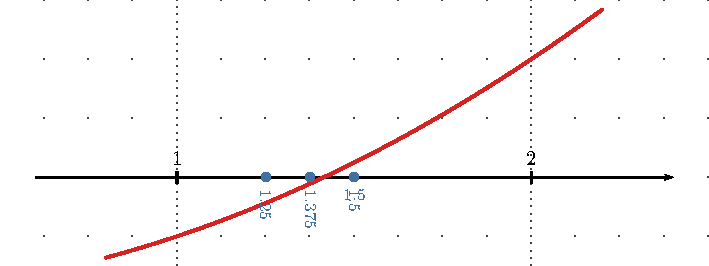
\includegraphics[scale=1]{Chapitre_3_analyse_numerique/figures/fig_5/fig_5.pdf}

\smallskip
\begin{minipage}{0.9\textwidth}
\begin{center}
\fig{On encadre de plus en plus précisément la valeur du zéro positif de la fonction $f(x)=x^2-2$.}
%\textit{\small On encadre de plus en plus précisément la valeur du zéro positif de la fonction $f(x)=x^2-2$ }
\end{center}
\end{minipage}
\end{center}

\smallskip
En poursuivant, on obtient les valeurs suivantes pour les 8 premières étapes :
$$
\begin{array}{ll}
  a_0 = 1			& b_0 = 2 \\
  a_1 = 1			& b_1 = 1,5 \\
  a_2 = 1,25		& b_2 = 1,5 \\
  a_3 = 1,375		& b_3 = 1,5 \\
  a_4 = 1,375		& b_4 = 1,4375 \\
  a_5 = 1,40625		& b_5 = 1,4375 \\
  a_6 = 1,40625		& b_6 = 1,421875 \\
  a_7 = 1,4140625	& b_7 = 1,421875 \\
  a_8 = 1,4140625\eh{3}	& b_8 = 1,41796875 \\
\end{array}
$$

Donc en $8$ étapes on obtient l'encadrement :
$$1,414  \leqslant \sqrt{2} \leqslant 1,417$$

Ce qui permet de déduire les deux premières décimales :
$\sqrt{2}\simeq 1,41$


\bigskip
\begin{boxexstheorieligne}
\begin{enumerate}[label=\textbf{E\thechapter.\arabic*},itemsep=4mm,series=refexercices]
\item En vous inspirant de l'exemple précédent, calculer à la main (calculatrice autorisée) un encadrement au dixième près (première décimale correcte) de $\sqrt{3}$.
\item Selon vous, serait-il plus efficace, d'un point de vue de la complexité de l'algorithme, de diviser les intervalles en 4 plutôt qu'en 2? Justifier votre réponse.
\item Écrire un programme en python qui détermine une approximation des zéros d'une fonction $f$ par la méthode de la dichotomie. On implémentera :
\vspace{-1mm} 
\begin{itemize}
\item une fonction python qui renvoie l'image d'une fonction $f$ donnée ({\small par exemple $f(x)=x^2-2$}).
\item une fonction python \comp{dichotomie\_etape(a,b,n)} qui prend en paramètre les nombres $a$ et $b$ ($a\leqslant b$) ainsi que le nombre d'étapes $n$ désiré.\\
La fonction renvoie les valeurs de $a$ et $b$ à la $n$\up{ième} étape.
\end{itemize}
\item Modifier la fonction \comp{dichotomie\_etape(a,b,n)} de l'exercice précédent pour qu'elle affiche également les valeurs de $a$ et $b$ à chaque étape.
\item\label{dicho_racine_2} En vous aidant de la fonction \comp{dichotomie\_etape(a,b,n)} et en utilisant la fonction définie par $f(x)=x^2-2$ sur l'intervalle $[1;2]$, faire des essais pour plusieurs valeurs de $n$ pour déterminer le nombre d'étapes nécessaires pour obtenir la 5\up{ième} décimale correcte de $\sqrt{2}$.
\item Vérifier que $x=2$ est un zéro de la fonction $f(x)=4x^4-12x^3+x^2+12x+4$.\\
Peut-on appliquer l'algorithme de dichotomie pour déterminer ce zéro ? 
\end{enumerate}
\end{boxexstheorieligne}



%\begin{tikzpicture}[remember picture,overlay]
%\path[left color=orange,right color=white]
%([yshift=-30pt]current page.north west)
%+(0,-2pt) rectangle +(14cm,2pt); 
%
%\path[left color=orange,right color=white]
%([yshift=-175pt,xshift=+14cm]current page.north west)
%+(0,-.5pt) rectangle +(5.1cm,0.5pt);
%\end{tikzpicture}


%%---------------------------------------------------------------
%\subsection{Résultats numériques pour $(1,10)^{1/12}$}
%
%
%Nous cherchons maintenant une approximation de $(1,10)^{1/12}$.
%Soit $f(x) = x^{12} - 1,10$.
%On pose $a_0=1$ et $b_0=1,1$. Alors $f(a_0)=-0,10 \le 0$ et $f(b_0)=2,038\ldots \ge 0$.
%
%$$
%\begin{array}{ll}
%  a_0 = 1             & b_0 = 1,10 \\
%  a_1 = 1             & b_1 = 1,05 \\
%  a_2 = 1             & b_2 = 1,025 \\
%  a_3 = 1             & b_3 = 1,0125 \\
%  a_4 = 1,00625       & b_4 = 1,0125 \\
%  a_5 = 1,00625       & b_5 = 1,00937\ldots\\
%  a_6 = 1,00781\ldots & b_6 = 1,00937\ldots \\
%  a_7 = 1,00781\ldots & b_7 = 1,00859\ldots \\
%  a_8 = 1,00781\ldots & b_8 = 1,00820\ldots \\
%\end{array}
%$$
%
%Donc en $8$ étapes on obtient l'encadrement :
%$$ 1,00781 \le (1,10)^{1/12} \le 1,00821$$



%---------------------------------------------------------------
\subsection{Calcul de l'erreur}

La méthode de dichotomie fournit un encadrement d'un zéro de $f(x)$ et, par construction, la longueur de l'intervalle à l'étape $n$ représente l'erreur maximale commise dans l'estimation du zéro (à l'étape $n$). On appelle cette erreur maximale  la \textbf{précision} de l'approximation du zéro.

\smallskip
Nous remarquons que la précision augmente d'un facteur 2 d'une étape à l'autre car la taille de l'intervalle contenant le zéro est divisée par $2$.

%Au départ, on sait que $\ell \in [a,b]$ (de longueur $b-a$) ;
%puis $\ell  \in [a_1,b_1]$ (de longueur $\frac{b-a}{2}$) ;
%puis $\ell \in [a_2,b_2]$ (de longueur $\frac{b-a}{4}$) ; ... ;
%$[a_n,b_n]$ étant de longueur $\frac{b-a}{2^n}$.

\medskip
Concrètement, si $x_0$ est un zéro de la fonction $f$ dans l'intervalle $[a;b]$, alors on sait que $a_n \leqslant x_0 \leqslant b_n$ et donc $$|x_0-a_n| \leqslant |b_n-a_n| = \frac{b-a}{2^n}$$

Pour obtenir une approximation de $x_0$ avec une précision de $10^{-N}$, il faut choisir $n$ tel que  $\frac{b-a}{2^n} \leqslant 10^{-N}$ :

\setlength{\jot}{3mm}
\hspace*{2cm}\begin{minipage}{0.6\textwidth}\begin{align*}
\frac{b-a}{2^n} \leqslant 10^{-N}
 & \ssi[2] (b-a)10^N \leqslant 2^n  \\
 & \ssi[2] \log(b-a) + \log(10^N)  \leqslant \log(2^n) \\
 & \ssi[2] \log(b-a) + N \leqslant n \log(2) \\
 & \ssi[2] n \geqslant \frac{N +  \log(b-a)}{\log(2)} \\
\end{align*}\end{minipage}

\vspace{-2mm}
Il faut donc que $n \geqslant \frac{N +  \log(b-a)}{\log(2)}$ pour obtenir une précision de $N$ chiffres après la virgule. 
%Sachant $\log(2) \simeq 0,301$, si par exemple $b-a \leqslant 1$, voici le nombre d'itérations suffisantes pour avoir une  précision de $10^{-N}$ (ce qui correspond, à peu près, à $N$ chiffres exacts après la virgule).
%\begin{center}
%\begin{tabular}{ll}
%  $10^{-10}$ ($\sim 10$ décimales) &  $34$ itérations \\
%  $10^{-100}$ ($\sim 100$ décimales) &  $333$ itérations \\
%  $10^{-1000}$ ($\sim 1000$ décimales) &  $3322$ itérations \\
%\end{tabular}
%\end{center}
%
%On remarque qu'il faut entre $3$ et $4$ itérations supplémentaires pour obtenir une nouvelle décimale.

\bigskip
\begin{remarque}
En toute rigueur il ne faut pas confondre précision et nombre de décimales exactes.\\
Par exemple $0,999$ est une approximation de $1$ à $10^{-3}$ près, mais aucune
décimale après la virgule n'est exacte.  En pratique, c'est la précision qui est la plus importante, mais il est plus\\ \guillemets{frappant} de parler du nombre de décimales exactes.
\end{remarque}





\bigskip
\begin{boxexstheorieligne}
\begin{enumerate}[label=\textbf{E\thechapter.\arabic*},itemsep=4mm,resume=refexercices]
\item En supposant $b-a\leqslant 1$, calculer à la main (calculatrice autorisée) le nombre minimum d'étapes qu'il faut effectuer pour obtenir une précision de :
\begin{multicols}{3}
\begin{enumerate}[label=\roman*)]
\item $10^{-10}$ {\footnotesize($\sim 10$ décimales)}
\item $10^{-100}$ {\footnotesize($\sim 100$ décimales)}
\item $10^{-1000}$ {\footnotesize($\sim 1000$ décimales)}
\end{enumerate}
\end{multicols}
\item Avec les même conditions que l'exercice précédent, combien faut-il d'étapes pour gagner une décimale de précision? 
\item\label{dicho_prec} Écrire un programme en python qui détermine une approximation des zéros d'une fonction $f$ par la méthode de la dichotomie avec la précision désirée. On implémentera :
\vspace{-1mm} 
\begin{itemize}
\item une fonction python \comp{dichotomie\_precision(a,b,precision)} qui prend en paramètre les nombres $a$ et $b$ ($a\leqslant b$) ainsi que la \textit{precision} désirée.\\
La fonction renvoie les valeurs de $a$ et $b$.
\end{itemize}
\item Après avoir localisé des intervalles approprié (graphique avec geogebra autorisé), déterminer tous les zéros des fonction suivantes en vous servant du programme de l'exercice \ref*{dicho_prec} :
\begin{multicols}{2}
\begin{enumerate}[label=\roman*)]
\item $f(x)=e^{x-1}-\frac{x^4}{4}$\eh{3} \textit{(précision : $10^{-3}$)}
\item $g(x)=\sin^2(x)+\frac{\phantom{^4}x\phantom{^4}}{3}$\eh{3} \textit{(précision : $10^{-4}$)}
\end{enumerate}
\end{multicols}
%\item Que fait la fonction \comp{mystere} ci-dessous :
%
%\insertcode{Algos/mystere.py}{fonction.py}{0.65}
%\item En vous aidant de la fonction \comp{dichotomie\_etape(a,b,n)} et en faisant des essais pour plusieurs valeurs du nombre d'étapes $n$, déterminer le nombre d'étapes nécessaires pour obtenir une précision de $10^{-5}$ (la 5\up{ième} décimale est correcte) de $\sqrt{2}$.
\end{enumerate}
\end{boxexstheorieligne}



























































%%---------------------------------------------------------------
%\subsection{Algorithmes}
%
%Voici comment implémenter la dichotomie dans le langage Python. Tout d'abord
%on définit une fonction $f$ (ici par exemple $f(x)=x^2-10$) :
%
%%\insertcode{algos/dichotomie-tex1.py}{dichotomie.py (1)}
%
%Puis la dichotomie proprement dite : en entrée de la fonction, on a
%pour variables $a,b$ et $n$ le nombre d'étapes voulues.
%
%%\insertcode{algos/dichotomie-tex2.py}{dichotomie.py (2)}
%
%Même algorithme, mais avec cette fois en entrée la précision souhaitée :
%
%%\insertcode{algos/dichotomie-tex3.py}{dichotomie.py (3)}
%
%
%Enfin, voici la version récursive de l'algorithme de dichotomie.
%
%%\insertcode{algos/dichotomie-tex4.py}{dichotomie.py (4)}
%
%
%%---------------------------------------------------------------
%%\subsection{Mini-exercices}
%
%%\begin{miniexercices}
%\begin{enumerate}
%  \item \`A la main, calculer un encadrement à $0,1$ près de $\sqrt{3}$.
%  Idem avec $\sqrt[3]{2}$.
%
%  \item Calculer une approximation des solutions de l'équation $x^3+1=3x$.
%
%  \item Est-il plus efficace de diviser l'intervalle en $4$ au lieu d'en $2$ ?
%  (\`A chaque itération, la dichotomie classique nécessite l'évaluation de $f$ en une nouvelle valeur
%  $\frac{a+b}{2}$ pour une précision améliorée d'un facteur $2$.)
%
%  \item \'Ecrire un algorithme pour calculer plusieurs solutions de $(f(x)=0)$.
%
%  \item On se donne un tableau trié de taille $N$, rempli de nombres appartenant à $\{1,\ldots,n\}$.
%  \'Ecrire un algorithme qui teste si une valeur $k$ apparaît dans le tableau et en quelle position.
%
%\end{enumerate}
%%\end{miniexercices}

















%\section{Méthode de Newton}

\subsection{Principe de la méthode de Newton}
La méthode de Newton consiste à \guillemets{linéariser} la fonction $f$ autour d'un valeur $u_0$; on va approximer la fonction par sa tangente et chercher un zéro $u_1$ de cette droite (qui est la \guillemets{linéarisation} de la fonction). On recommence le procédé avec la valeur $u_1$ et ainsi de suite autant de fois que nécessaire. On obtient alors une suite $(u_n)_{n\in \N}$ qui sont les zéros des tangentes successives et qui \guillemets{normalement} converge vers un zéro de $f$.

\medskip
Soit $f:[a,b] \to \R$ une fonction dérivable et $u_0 \in[a,b]$.
On appelle $(u_1,0)$ l'intersection de
la tangente au graphe de $f$ en $(u_0,f(u_0))$ avec l'axe des abscisses.
Si $u_1 \in[a,b]$ alors on recommence l'opération avec la tangente au point d'abscisse $u_1$.
Ce processus conduit à la définition d'une suite récurrente :
$$u_0 \in [a,b] \qquad \text{ et } \qquad u_{n+1} = u_n - \frac{f(u_n)}{f'(u_n)}.$$


En effet, la tangente au graphe de $f$ au point d'abscisse $u_n$ est donnée par la fonction
$$d(x) = f'(u_n)(x-u_n)+f(u_n)$$

\vspace{-4mm}
 Il est facile de déterminer que :

\vspace{-4mm}
$$d(x)=0\ssi[3] 0=f'(u_n)(x-u_n)+f(u_n) \ssi[3]  x=u_n - \frac{f(u_n)}{f'(u_n)}$$

Cette suite converge, sous certaine conditions, vers un zéro de la fonction $f$.

\begin{center}
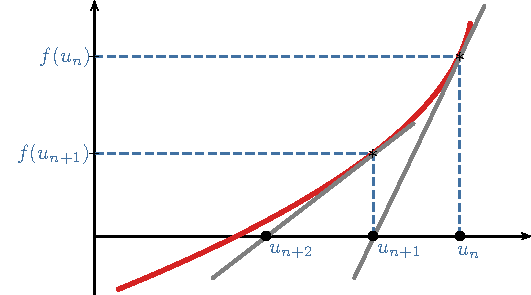
\includegraphics[scale=1]{Chapitre_3_analyse_numerique/figures/fig_6/fig_6.pdf}

\smallskip
\begin{minipage}{0.8\textwidth}
\begin{center}
\textit{\small Les zéros des tangentes forment une suite convergeant vers un zéro de $f$. }
\end{center}
\end{minipage}
\end{center}


\medskip
Lorsque la méthode est applicable, elle est d'une redoutable efficacité. Mais pour que la suite $(u_n)_{n\in \N}$ converge il faut, entre autres conditions, que le point de départ de l'itération ne soit pas trop loin d'un zéro de la fonction. La méthode exige donc de connaître une \guillemets{approximation} de la valeur cherchée.

\medskip
Le résultat suivant, admis sans démonstration, donne les conditions suffisantes pour que la suite converge : 


\begin{theoreme}[\small \textit{convergence de Newton}]\label{convergence_newton}
Soit $f:]a,b[ \to \R$ une fonction deux fois dérivable dont la deuxième dérivée est continue. \\
Si $c\in]a;b[$ est une racine de la fonction $f$ et que $f'(c)\neq 0$, alors il existe $L\in\R$ tel que la suite 
$$u_{n+1}=u_n - \frac{f(u_n)}{f'(u_n)}$$
converge vers $c$ pour tout $u_0\in[c-L;c+L]$.
\end{theoreme}

\begin{minipage}[t][][b]{0.6\textwidth}
Le théorème \ref*{convergence_newton} donne les conditions sur la fonction $f$ pour que la méthode de Newton converge si le point de départ n'est pas trop loin du zéro cherché.

\medskip
Bien que le théorème affirme de l'existence d'un intervalle de convergence, il ne fournit pas d'information sur la longueur de cet intervalle. La longueur de l'intervalle peut-être très petite, et il s'avère parfois utile de recourir à d'autres méthodes pour avoir une première estimation d'un zéro.

\medskip
L'exemple ci-contre montre la méthode de Newton appliquée à la fonction $f$ donnée par :
$$f(x)=\frac{x^3-6x^2+6x+24}{4}$$ 
\end{minipage}\hspace{5mm}\begin{minipage}[t][][b]{0.4\textwidth}
\begin{center}
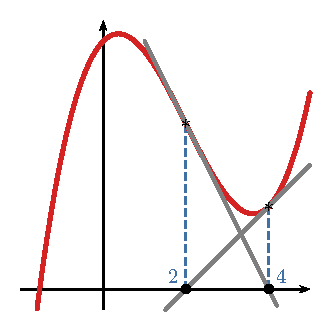
\includegraphics[scale=1]{Chapitre_3_analyse_numerique/figures/fig_7/fig_7.pdf}

\textit{\small La méthode de Newton échoue si $u_0=2$. }
\end{center}
\end{minipage}

\bigskip
Cette fonction possède un zéro en $x\simeq -1,54$, mais si nous initions la méthode avec $u_0=2$ alors la suite qui en résulte oscille entre les valeur $2$ et $4$.

%---------------------------------------------------------------
\subsection{Cas particulier : Calcul de $\sqrt{a}$}

Si on cherche à calculer $\sqrt{a}$, on peut poser $f(x)=x^2-a$ et $f'(x)=2x$. La suite issue de la méthode de Newton pour cette fonction est déterminée par $u_0>0$ et la relation de récurrence : $$u_{n+1} = u_n - \frac{u_n^2-a}{2u_n}$$
Cette suite s'appelle \textbf{suite de Héron}\footnote{Héron d'Alexandrie, mathématicien grec du 1\up{er} siècle après J.C., est connu pour sa formule permettant de calculer l'aire d'un triangle en utilisant la longueur de ses côtés. Cette formule nécessite néanmoins de calculer une racine carrée.} et la proposition \ref*{prop:heron} ci-dessous montre qu'elle converge vers $\sqrt{a}$.


%\begin{exstheorie}
%\begin{enumerate}[label=\textbf{E\thechapter.\arabic*},itemsep=2mm]\setcounter{enumi}{11}
%\item\label{alternative:Heron} Démontrer que la suite de Héron peut s'écrire :  $$u_{n+1} = \frac12 \left(u_n+\frac{a}{u_n}\right)\;$$ et que $u_n\geqslant 0 \eh[2] \forall n\in \N$ (pour  $a,u_0>0$). 
%\end{enumerate}
%\end{exstheorie}




\bigskip
\begin{proposition}
\label{prop:heron}
Pour $a>0$, la suite de Héron définie par $u_{n+1} = u_n - \frac{u_n^2-a}{2u_n}$
 converge vers $\sqrt{a}$ pour tout $u_0>0$.
\end{proposition}

%\textit{Démonstration :}
\begin{demonstration}
\medskip
Soit $u_0>0.$ La suite de Héron peut s'écrire $u_{n+1} = \frac12 \left(u_n+\frac{a}{u_n}\right)$ {\small (voir exercice \ref*{alternative:Heron})}.

\smallskip
Commençons par montrer que $u_n^2 \geqslant a$ pour $n\geqslant 0$. En effet :

$$u_{n+1}^2-a = \frac14 \left(\frac{u_n^2 + a}{u_n}\right)^2 - a = \frac{1}{4u_n^2}(u_n^4-2au_n^2+a^2)=\frac14 \frac{(u_n^2-a)^2}{u_n^2}\geqslant 0$$

Donc $u_{n+1}^2 - a \geqslant 0$ et par conséquent $u_{n}^2 \geqslant a$ pour tout $n\geqslant 0$.

\medskip
Montrons maintenant que $(u_n)_{n\ge1}$ est une suite décroissante. Nous avons :

$$\frac{u_{n+1}}{u_n} = \frac12 \left(1+\frac{a}{u_n^2}\right)$$

\smallskip
et pour $n\geqslant 0$, nous savons que $u_n^2 \geqslant a$ (donc $\frac{a}{u_n^2}\leqslant 1$). Il suit que $\frac{u_{n+1}}{u_n} \leqslant 1$ pour tout $n\leqslant 0$.

\medskip
La suite $(u_n)_{n\ge0}$ est donc décroissante et comme $u_n\geqslant 0$ {\small (voir exercice \ref*{alternative:Heron})} pour tout $n\geqslant 0$, alors la suite est également minorée par $0$. Donc elle converge.\clearpage

\medskip
Notons $\ell$ la limite de la suite $(u_n)_{n\in\N}$. Alors :

\smallskip
$$ u_{n+1} = \frac12 \left(u_n+\frac{a}{u_n}\right) \eh{2}\Rightarrow\eh{2}
 \limn{+\infty}{u_{n+1}}= \limn{+\infty}{\frac12 \left(u_n+\frac{a}{u_n}\right)} \eh{2}\Rightarrow\eh{2} \ell = \frac12 \left(\ell+\frac{a}{\ell}\right)$$ 

On trouve alors facilement que  $\ell^2=a$ et comme les termes de la suites sont positifs on a $\ell = \sqrt{a}$.

\vspace{-3mm}
\hfill $\blacksquare$
\end{demonstration}



\bigskip
\begin{boxexstheorieligne}
\begin{enumerate}[label=\textbf{E\thechapter.\arabic*},itemsep=2mm,resume=refexercices]
\item\label{alternative:Heron} Démontrer que la suite de Héron peut s'écrire :  $$u_{n+1} = \frac12 \left(u_n+\frac{a}{u_n}\right)\;$$ et que $u_n\geqslant 0 \eh{2} \forall n\in \N$ (pour  $a,u_0>0$). 
\item Calculer à la main et sans logiciel une approximation de $\sqrt{2}$ en effectuant 4 itérations de la méthode de Newton avec comme point de départ la valeur $u_0=1$.\\ Combien de décimales sont correctes dans cette approximation?
\item Comparer les résultats de l'exercice précédent avec le résultat de l'exercice \ref*{dicho_racine_2}.\\ Que concluez-vous?
\item Écrire un programme en Python d'une fonction \comp{racine\_carree(a\!;d\!;n)} qui calcule la racine de la valeur \comp{a} en utilisant la suite de Héron. 
\begin{itemize}
\item \comp{d} est la valeur de départ de l'itération,
\item \comp{n} est le nombre d'itérations désirés,
\item la fonction renvoie la valeur estimée du zéro à chaque étape.
\end{itemize}
\item Peut-on appliquer la méthode de Newton à la fonction $\sqrt[3]{x}$ ?
\end{enumerate}
\end{boxexstheorieligne}
\clearpage







%\section{Méthode du point fixe}

\subsection{Principe de la méthode du point fixe}
Il est parfois possible de résoudre de manière itérative des équations de la forme $$g(x)=x$$

Les solutions de cette équation sont appelées les \guillemets{points fixes} de  $g$. Elles représentent les préimages qui sont invariantes par $g$ ou, de manière équivalente, les valeurs ou $g$ intersecte la fonction identité.

\medskip
Il est clair qu'il est toujours possible de ramener la recherche d'un zéro d'une fonction $f$ à la recherche d'un point fixe d'une fonction $g$; il suffit, par exemple, de poser $g(x)=f(x)+x$ et dans ce cas :
$$f(x)=0 \ssi[3] g(x)=x$$
Cependant et comme nous aurons l'occasion de le constater, bien que le fait de définir $g(x)=f(x)+x$ semble naturel, ce choix ne sera pas toujours le meilleur.


\medskip
\begin{minipage}[t][][b]{0.6\textwidth}
La \textit{méthode du point fixe} consiste à construire une suite $\left(x_{n}\right)_{n\in\N}$ définie par :
$$x_{n+1}=g(x_n) \eh{3}\textrm{et $x_0$ est choisit arbitrairement}$$

\medskip
Il est intéressant de comprendre à l'aide d'un graphique le mécanisme de convergence de cette suite. \\
Si la \guillemets{variation} de la fonction n'est pas trop importante autour d'un éventuel point fixe, alors nous obtenons une succession de valeur qui vont être \guillemets{attirée} par le point fixe.


 
\end{minipage}\hspace{5mm}\begin{minipage}[t][][b]{0.4\textwidth}
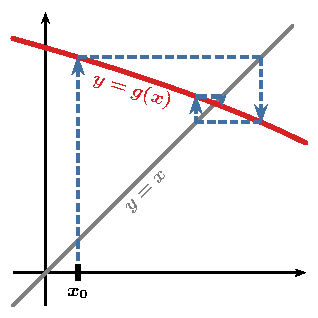
\includegraphics[scale=1]{Chapitre_3_analyse_numerique/figures/fig_9/fig_9.pdf}
\end{minipage}


%\medskip
%Cette méthode est motivée par la résultat du théorème \ref*{prop:point_fixe}, qui assure qu'en cas de convergence de cette suite, la valeur de convergence est un point fixe de la fonction $g$.
%
%\medskip
%\begin{proposition}
%\label{prop:point_fixe}
%Soit $g:[a;b]\rightarrow [a;b]$ une fonction continue et $x_0\in [a;b]$.\\
%Supposons que la suite $(x_n)_{n\ge0}$ définie comme ci-dessus converge vers $\ell$. Alors :
% 
%$$\ell=g(\ell)$$
% 
%et donc $\ell$ est un point fixe de $g$.
%\end{proposition}
%
%\begin{demonstration}
%
%\medskip
%Ce théorème découle directement d'une propriété des fonctions continues qui n'est pas au programme de mathématique du collège. Il est possible de montrer que si $g$ est une fonction continue et que $\left(a_n\right)_{n\ge0}$ est une suite qui converge (vers $\ell\in\R$), alors :
%$$g(\lin{\infty}a_n)=\lin{\infty}g\left(a_n\right)$$
%Par conséquent, $g(\ell)=g(\lin{\infty}a_n)=\lin{\infty}g\left(a_n\right)=\lin{\infty}a_{n+1}=\ell$.
%
%\vspace{-3mm}
%\hfill $\blacksquare$
%\end{demonstration}


%\subsection{Convergence de la suite $x_{n+1}=g(x_n)$}

La proposition suivante établit les conditions suffisantes pour que la suite définie par $x_{n+1}=g(x_n)$ converge vers un point fixe de $g$.

\begin{proposition}
\label{prop:existence_point_fixe}
Soit $g : [a, b] \rightarrow [a, b]$ une fonction continue sur $[a;b]$ et dérivable sur $]a;b[$.\\
Supposons que
$$\vert g^\prime(x)\vert \leqslant K \eh{3}\forall x \in [a, b] \eh{3} \textrm{avec}\eh{2} 0 \leqslant K < 1$$  
Alors, $g$ possède un unique point fixe dans l'intervalle $[a;b]$ et pour tout $x_0 \in [a, b]$ , la suite définie par
\mbox{$x_{n+1} = g(x_n)$} converge vers ce point fixe.
\end{proposition}

\medskip
\begin{demonstration}
Soit $x_0\in[a;b]$ et remarquons qu'on a par hypothèse :
$$g(x)\in[a;b]\eh{2} \forall x\in[a;b]$$
donc la suite $x_{n+1}=g(x_n)$ est bien définie.

\medskip
On définit la fonction $h(x)=g(x)-x$. Nous avons que :

\begin{itemize}
\item $h(x)$ est une fonction continue sur l'intervalle $[a;b]$.
\item $h(a)=g(a)-a\geqslant 0$ car $g(a)\in[a;b]$ et donc $g(a)\geqslant a$.
\item $h(b)=g(b)-b\leqslant 0$ car $g(b)\in[a;b]$ et donc $g(b)\leqslant b$.
\end{itemize}

Le théorème \ref*{thm_valeurs_intermediaires} des valeurs intermédiaires assure que $h$ possède un zéro $\ell$ à l'intérieur de l'intervalle $[a;b]$ et $\ell$ est donc un point fixe de $g$ ($g(\ell)=\ell$).

\medskip
Par ailleurs $h'(x)=g'(x)-1< 1-1=0$ et la fonction $h$ est donc strictement décroissante. Ceci garantit que $\ell$ est l'unique zéro de $h$ et donc l'unique point fixe de $g$.

\bigskip
Il reste à montrer que la suite définie par $x_{n+1} = g(x_n)$ converge vers $\ell$, c'est-à-dire $\lin{\infty}\vert x_{n+1}-\ell\vert =0$.

\medskip
La fonction $g$ vérifie les hypothèses du théorème des accroissements finis sur $[a;b]$. Donc pour chaque valeur de $n$, il existe $c_n\in [a;b]$ tel que :

$$\vert g(x_{n})-g(\ell)\vert =\vert g'(c_n)\cdot (x_n-\ell)\vert \implique[3] \vert x_{n+1}-\ell\vert=\vert g'(c_n)\cdot (x_n-\ell)\vert$$


\medskip
Comme par hypothèse $\vert g'(c_n)\vert\leqslant K$, alors :

$$\vert x_{n+1}-\ell\vert \leqslant K\cdot \vert (x_n-\ell) \vert$$

Par récurrence on a : 
$$\vert x_{n+1}-\ell\vert \leqslant K^n\cdot \underbrace{\vert (x_0-\ell)\vert}_{=\textrm{ constante}}  \eh{3}\forall n\in\N$$


Comme $0\leqslant K< 1$, on obtient : 
$$\lin{\infty}  \vert x_{n+1}-\ell\vert \leqslant \lin{\infty}K^n\cdot \vert (x_0-\ell)\vert=0$$

\vspace{-3mm}
\hfill $\blacksquare$
\end{demonstration}

%\begin{exemple}
%%On souhaite résoudre l'équation $\frac{\sin(x)-x+1}{2}=0$. On trouve à l'aide d'un logiciel graphique que cette 
%%
%%\medskip
%%On montre facilement que $f(x)=0\ssi[2]\frac{\sin(x)+x+1}{2}=x$.
%%
%%\medskip
%On considère la fonction $f(x)=\frac{\sin(x)+x+1}{2}$ sur l'intervalle $[1;2]$ qui est dérivable.
%
%\medskip
%On calcule $f'(x)=\frac{\cos(x)+1}{2}$ et on constate que $0<f'(x)<1$ pour $x\in[1;2]$. En effet :
%
%$$x\in[1;2] \implique[2] 0<\cos(x)<1 \implique[2] 1<\cos(x)+1<2 \implique[2] 0<\frac{\cos(x)+1}{2}<1$$
%
%
%\medskip
%On conclut que $\vert f'(x)\vert <1$ si $x\in[1;2]$ et comme $f'(x)>0$ pour $x\in [1;2]$, on déduit que $f$ est croissante sur cet intervalle.
%
%\medskip
%De plus, $f(1)>1$ et $f(2)<2$. Par conséquent on a forcément $f:[1;2]\rightarrow [1;2]$ et toutes les hypothèses du théorème \ref*{prop:existence_point_fixe} sont vérifiées. %(Le point fixe est $\ell\cong 1,9346$) 
%\end{exemple}

\bigskip
\begin{remarques}\label{rem:critère_pt_fixe}
\item Il est possible de montrer (à l'aide du développement en série de Taylor d'ordre 1) que l'erreur commise avec la méthode du point fixe à l'étape $n+1$ est d'\textbf{environ} $\varepsilon \simeq\vert x_{n+1}-x_n \vert$, ce qui fournit \textbf{un critère d'arrêt} (précision) lors de la programmation de la méthode du point fixe.
%\item L'hypothèse que $g$ est une fonction de $[a;b]$ dans $[a,b]$ ne doit pas être minimisée. Avec la continuité de $g$, cette hypothèse garantit que la fonction $g$ possède bien un point fixe. 
%\item Soit $g$ une fonction dérivable et supposons que $\ell$ est un point fixe de de $g$. Si $\ell\in ]a;b[$ et que $\vert g^\prime(x)\vert \leqslant K<1 \eh{3}\forall x \in [a, b]$, alors il existe un intervalle $[c;d]\subset [a;b]$ telle que $g:[c;d]\rightarrow[c,d]$. 

%\item Si $\ell \in ]a, b[$ est un point fixe de $g$, que $g$ est une fonction continue, dérivable sur $[a;b]$ et telle que $\vert g^\prime(x)\vert \leqslant K<1 \eh{3}\forall x \in [a, b]$, alors il existe un intervalle $[c;d]\subset [a;b]$ tel que $g:[c;d]\rightarrow[c,d]$. Il est donc possible d'appliquer la méthode du point fixe à $g$.
\item\label{rem:critère_pt_fixe_ii} Si $\ell$ est un point fixe de $g$, que $g$ est une fonction continument  dérivable\footnote{dont la dérivée est continue.} dans un voisinage de $\ell$ et telle que $\vert g^\prime(\ell)\vert <1$, alors il existe un intervalle $[a;b]$ contenant $\ell$ tel que $g:[a;b]\rightarrow[a,b]$ et $\vert g^\prime(\ell)\vert <1 \eh{2}\forall x\in [a;b]$. Il est donc possible d'appliquer la méthode du point fixe à $g$.
\end{remarques}


\begin{boxexstheorieligne}

%\vspace{-4mm}
\begin{enumerate}[label=\textbf{E\thechapter.\arabic*},itemsep=8mm,resume=refexercices]

%% EXERCICE
\item Soit la fonction $f(x)=x^2-x-2$ dont les zéros sont $-1$ et $2$. On considère les fonctions :
$$g_1(x)=x^2-2\eh{6} g_2(x)=\sqrt{2+x}\eh{6}g_3(x)=1+\frac{2}{x} \eh{6}g_4(x)=x+\log(x^2-x-1)$$
\begin{enumerate}[label=\roman*)]
\item Donner le domaine de définition des fonctions $g_k\eh{1}, \eh{1}k\in\{1;2;3;4\}$.
\item Montrer que la recherche des zéros de $f$ revient à trouver les points fixes de chacune des fonctions $g_k\eh{1}, \eh{1}k\in\{1;2;3;4\}$.
%\item Déterminer les zéros de $f$.
\item A l'aide de la remarque 2.\ref*{rem:critère_pt_fixe_ii}, déterminer pour quels fonctions $g_k\eh{1}, \eh{1}k\in\{1;2;3;4\}$, il est possible d'appliquer la méthode du point fixe. Donner une réponse par zéro de $f$.
\end{enumerate}
%\pagebreak




%% EXERCICE
\item Écrire un programme en Python d'une fonction \comp{point\_fixe(a;n)} qui calcule une approximation au bout de $n$ itérations d'un zéro d'une fonction $f$ en utilisant la méthode du point fixe : 
\vspace{-5mm}
%\begin{multicols}{2}
\begin{itemize}[left=0mm, itemsep=1mm]
\item \comp{a} est la valeur de départ,
\item \comp{n} est le nombre d'itérations désirés,
\item on utilise une boucle \comp{for} pour l'itération,
\item la fonction renvoie une estimation du zéro.
\end{itemize}
%\end{multicols}






%% EXERCICE
\item Écrire une fonction \comp{point\_fixe\_precision(a;precision)} qui calcule une approximation avec une certaine précision d'un zéro d'une fonction $f$ (préalablement définie) en utilisant la méthode du  point fixe  ?
\begin{itemize}\setlength{\itemsep}{1mm}
\item \comp{a} est la valeur de départ,
\item \comp{precision} est la précision désirée ($0,1 \pvirg{1} 0,01 \pvirg{1} 0,001 \pvirg{1}$ ...),
\item on utilisera une boucle \comp{while} pour l'itération,
\item la fonction renvoie la valeur estimée du zéro ainsi que le nombre $n$ d'itérations effectuées.
\end{itemize}






%% EXERCICE
\item On cherche à comparer les méthodes de Dichotomie, de Newton et du Point fixe pour déterminer le zéro de la fonction $f$ suivante :
$$f(x)=\frac{10x-2\sin(x)-5}{10} \eh{5}(x\;\textrm{\it en radians})$$

\begin{enumerate}[label=\alph*),itemsep=2mm]
\item Utiliser Python pour tracer le graphique de $f$ dans l'intervalle $[\textstyle\frac{1}{2};1]$ et vérifier que $f$ possède un zéro dans cet intervalle.
\item Initier la méthode de dichotomie sur cet intervalle et donner le nombre d'étapes nécessaires pour obtenir une précision d'ordre $10^{-7}$.
\item Initier la méthode de Newton sur cet intervalle (prendre $x_0=1$) et donner le nombre d'étapes nécessaires pour obtenir une précision d'ordre $10^{-7}$. 
\item \begin{enumerate}[label=\roman*)]
\item  Montrer que $g(x)=f(x)+x$ n'est pas un bon choix pour la fonction $g$ afin d'appliquer la méthode du point fixe.
\item Montrer que $f(x)=0 \ssi[2] 0,2\sin(x)+0,5=x$ et montrer que la fonction définie par $g(x)=0,2\sin(x)+0,5$ vérifie toutes les hypothèses du théorème de convergence du point fixe sur l'intervalle $[\textstyle\frac{1}{2};1]$.
\item Initier la méthode du point fixe sur cet intervalle (prendre $x_0=1$) et donner le nombre d'étapes nécessaires pour obtenir une précision d'ordre $10^{-7}$. 
\end{enumerate} 
\end{enumerate}

%Initier la méthode de dichotomie sur cet intervalle et prendre $x_0=1$ pour la méthode de Newton et du Point Fixe.
%
%\medskip
%Combien d'étapes sont nécessaires pour obtenir une précision d'ordre $10^{-7}$ avec chacune des 3 méthodes?






%%% EXERCICE
%\item On cherche à résoudre l'équation $\frac{\sin(x)-2x+1}{2}=0$
%\begin{enumerate}[label=\alph*),itemsep=2mm]
%\item Utiliser Python pour localiser une solution de l'équation dans l'intervalle $[0;1]$.
%\item Déterminer une \guillemets{bonne} fonction $g$ telle que $f(x)=0\ssi[2] g(x)=x$.
%
%Vérifier toutes les hypothèses du théorème du point fixe.
%\item Initier la méthode du point fixe sur cet intervalle (prendre $x_0=0,5$) et donner une approximation d'une solution de l'équation avec un précision d'ordre $10^{-3}$. 
%\end{enumerate} 
%
%
%
%
%
%
%
%% EXERCICE
\item Un nageur se trouve à une distance de $0,57$ kilomètres du rivage et aimerait rejoindre sa cabane.

\begin{minipage}[t][][b]{0.5\textwidth}
Il est positionné tel que le point $A$ est sa projection orthogonale sur le rivage et la distance séparant le point $A$ de la cabane est de $2,8\; km$.

\medskip
Le nageur peut nager a une vitesse de $3\;km/h$ et marcher sur le rivage à une vitesse de $5km/h$.
\end{minipage}
\begin{minipage}[t][][b]{0.6\textwidth}
\vspace*{-1mm}\includegraphics[scale=0.85]{Chapitre_3_analyse_numerique/figures/fig_8/fig_8.pdf}
\end{minipage}

\medskip
On souhaite déterminer à quelle distance de la cabane doit se trouver le point $P$, correspondant à l'endroit où le nageur doit sortir de l'eau, pour rejoindre la cabane en un minimum de temps.

\begin{enumerate}[label=\roman*),itemsep=1mm]
\item Modéliser la situation à l'aide d'une fonction $f$. {\small(Unités : kilomètres et heures)}
\item Utiliser \guillemets{Python} pour tracer le graphique de $f$.
\item Localiser les environs de(s) l'extremum(s) de $f$.
\item Déterminer un intervalle $[a;b]$ et une fonction $g$ dont on souhaite calculer le(s) point(s) fixe(s) et vérifier que cette fonction rempli les conditions de la méthode du point fixe sur l'intervalle.
\item Utiliser la méthode du point fixe pour déterminer le(s) extremum(s) de $f$.% sur un intervalle raisonnable au vu du point précédent.%\\{\small (Attention au choix de la fonction $g$ dont on veut déterminer le(s) point(s) fixes.)}
\item Conclure le résultat.
\end{enumerate}
%\hspace{5mm}

\end{enumerate}
\end{boxexstheorieligne}


%\newpage
%~
%\newpage
%\fancyhead[CO,CE]{\sc Réponses C-\thechapter\hspace{0.5mm}}
%\fontsize{10}{12}\selectfont
%\begin{center}
\textbsc{Réponses}
\end{center}

\everymath{\displaystyle}


\begin{enumerate}[label=R4.\arabic*, font=\bfseries, itemsep=8mm,labelsep*=4mm]
\item
%\leavevmode\vspace{-\dimexpr\baselineskip+\topsep}% Solution pour alignement trouvée sur https://tex.stackexchange.com/questions/456914/item-number-not-aligned-with-tasks
%\begin{minipage}[t][][b]{0.95\textwidth}
Choisissons la fonction $f(x)=x^2-3$ qui est continue sur $\mathbb{R}$ et dont l'unique zéro positif est $\sqrt{3}$.\\
Comme $1^2=1<3<4=2^2$ alors $1<\sqrt{3}<2$. Nous constatons également que $f(1)\cdot f(2)<0$ et donc $f$ change de signe dans l'intervalle $[1;2]$.

En appliquant l'algorithme de dichotomie dans l'intervalle $[1;2]$ nous obtenons les valeurs :
$$
\begin{array}{ll}
  a_0 = 1			& b_0 = 2 \\
  a_1 = 1,5			& b_1 = 2 \\
  a_2 = 1,5		& b_2 = 1,75 \\
  a_3 = 1,625		& b_3 = 1,75 \\
  a_4 = 1,6875		& b_4 = 1,75 \\
  a_5 = 1,71875		& b_5 = 1,75 \\
\end{array}
$$
Ce qui permet d'affirmer que $1,71<\sqrt{3}<1,75$ et donc $\sqrt{3}= 1,7...$






\item
Non, cela ne serait pas pus efficace. Bien que la précision à chaque étape soit améliorée d'un facteur 2, le nombre d'évaluations de la fonction est, en moyenne, doublé. Le bilan est donc nul.







\item
\insertcode{Chapitre_3_analyse_numerique/Programmes/fonction.py}{0.35}{}
\insertcode{Chapitre_3_analyse_numerique/Programmes/dichotomie_etape.py}{0.58}{}




\item
\insertcode{Chapitre_3_analyse_numerique/Programmes/dichotomie_etape_indiquee.py}{0.58}{}







\item
Il faut 18 étapes pour être sûr que la 5\up{ème} décimale soit correcte.






\item
On a $f(2)=4\cdot 2^4-12\cdot 2^3+2^2+12\cdot 2+4=0$.
Cependant, il n'est pas difficile de constater que $2$ est un zéro de multiplicité 2, c'est-à-dire que la fonction ne change pas de signe autour de $x=2$.

L'algorithme de dichotomie ne permet pas de localiser un tel zéro.






\item
Comme $0\leqslant b-a\leqslant 1$ alors $\log\left(b-a\right)\leqslant 0$. D'où $n\geqslant \frac{N}{\log(2)}$.
%\begin{multicols}{3}
\begin{enumerate}[label=\roman*), itemsep=3mm]
\item $n\geqslant \frac{10}{\log(2)}\simeq 34$ itérations.
\item $n\geqslant \frac{100}{\log(2)}\simeq 333$ itérations.
\item $n\geqslant \frac{1000}{\log(2)}\simeq 3321$ itérations.
\end{enumerate}
%\end{multicols}






\item
Le nombre d'étapes nécessaires pour obtenir une décimale supplémentaire de précision est de :
$$\frac{(N+1)+\log(b-a)}{\log(2)}-\frac{N+\log(b-a)}{\log(2)}=\frac{1}{\log(2)}\simeq 3.32$$
Il faut donc entre 3 et 4 étapes supplémentaires pour améliorer la précision d'une décimale.







\item
\insertcode{Chapitre_3_analyse_numerique/Programmes/dichotomie_precision.py}{0.58}{}







\item
\begin{enumerate}[label=\roman*),itemsep=4mm]
\item Geogebra montre que la fonction $f(x)=e^{x-1}-\frac{x^4}{4}$ \eh{1} a 3 zéros;

\medskip
$x_1\in[-1;0]$ \et{3}\comp{dichotomie\_precision(-1,0,0.001)} $\imply \eh{2} x_1\simeq -0.8837$%-0,8837\leqslant x_1\leqslant -0,8829$

\medskip
$x_2\in[1;2]$ \et{3}\comp{dichotomie\_precision(1,3,0.001)} $\imply \eh{2} x_2\simeq 1.6728$%1,6728\leqslant x_2\leqslant 1,6739$

\medskip
$x_3\in[7;8]$ \et{3}\comp{dichotomie\_precision(7,8,0.001)} $\imply \eh{2} x_3\simeq 7.8613$%7,8613\leqslant x_3\leqslant 7,8624$
\item La fonction $g(x)=\sin^2(x)+\frac{x}{3}$ \eh{1} a un zéro évident en $x_0=0$. Geogebra montre qu'elle possède 2 autres zéros;

\medskip
$x_1\in[-3;-2]$ \et{3}\comp{dichotomie\_precision(-3,-2,0.0001)} $\imply \eh{2} x_1\simeq -2.1369$%\leqslant x_1\leqslant -0,883$

\medskip
$x_2\in[-1;0]$ \et{3}\comp{dichotomie\_precision(-1,0,0.0001)} $\imply \eh{2} x_2\simeq -0.3470$%\leqslant x_2\leqslant 1,673$
\end{enumerate}

\bigskip
\textit{A noter que pour être certain d'avoir la précision désirée, il faut fournir une décimale supplémentaire.}





%\clearpage
\item $u_{n+1} = u_n - \frac{u_n^2-a}{2u_n}= \frac{2u_n}{2} - \frac{u_n^2-a}{2u_n} = \frac{1}{2}\left(2u_n - \frac{u_n\cdot \cancel{u_n}}{\cancel{u_n}}+\frac{a}{u_n} \right)=\frac{1}{2}\left(u_n + \frac{a}{u_n}\right)$







\item
\renewcommand{\arraystretch}{2.5}
\begin{minipage}[t][][b]{1\textwidth}\vspace{-8.5mm}
$\everymath{\textstyle}\begin{array}{l}
  u_0 = 1     \\
  u_1 = \frac12 \left(u_0+\frac{2}{u_0}\right) = \frac12\left(1+\frac{2}{1}\right) = \frac{3}{2} = 1,\textcolor{red!60!lightgray}{5} \\
  u_2 = \frac12 \left(u_1+\frac{2}{u_1}\right) = \frac12\left(\tfrac{3}{2}+\frac{2}{\tfrac{3}{2}}\right)
  = \frac{17}{12} = 1.41\textcolor{red!60!lightgray}{6}\ldots \\
  u_3 = \frac12 \left(u_2+\frac{2}{u_2}\right) = \frac12\left(\tfrac{17}{12}+\frac{2}{\tfrac{17}{12}}\right) = \frac{577}{408} = 1,41421\textcolor{red!60!lightgray}{5} \ldots \\
  u_4 = \frac12 \left(u_3+\frac{2}{u_3}\right) = \frac12\left(\tfrac{577}{408}+\frac{2}{\tfrac{577}{408}}\right) = 1,41421356237\textcolor{red!60!lightgray}{4}\ldots
\end{array}\everymath{\displaystyle}$
\end{minipage} 

\medskip
Pour $u_4$ on obtient $\sqrt{2} \simeq 1,41421356237$
avec $11$ décimales exactes.







\item
Avec la méthode de dichotomie il fallait effectuer 18 étapes pour obtenir 5 décimales correctes, alors que la méthode de Newton fournit déjà 11 décimales à la 4\up{ème} itération.\\
Sans équivoque, la méthode de Newton converge bien plus rapidement que la méthode de dichotomie vers un zéro de la fonction $f$. 







\item
\insertcode{Chapitre_3_analyse_numerique/Programmes/heron_racine_carree.py}{0.58}{}







\item
Non, on ne peut pas appliquer la méthode de newton à la fonction $\sqrt[3]{x}$ car la dérivée de la fonction dans n'importe quel intervalle contenant 0 n'est pas continue.







\item
\begin{enumerate}[label=\roman*),itemsep=3mm]
\item $D_{g_1}=\R$

\smallskip
$D_{g_2}=[-2;+\infty[$

\smallskip
$D_{g_3}=\R^{\ast}$

\smallskip
$\textstyle D_{g_4}=\R\setminus [\frac{1-\sqrt{5}}{2};\frac{1+\sqrt{5}}{2}]$
\item $g_1(x)=x \Rightarrow x^2-2=x \Rightarrow x^2-x-2=0$

\smallskip
$g_2(x)=x \Rightarrow \sqrt{2+x}=x \Rightarrow 2+x=x^2 \Rightarrow x^2-x-2=0$\\
\textit{\small (Valable uniquement pour le point fixe $x=2$. Pour $x=-1$ il faut considérer $-g_2(x)$.)}

\smallskip
$g_3(x)=x \Rightarrow 1+\frac{2}{x}=x \Rightarrow x+2=x^2 \Rightarrow x^2-x-2=0$

\smallskip
$g_4(x)=x \Rightarrow x+\log(x^2-x-1)=x \Rightarrow \log(x^2-x-1)=0 \Rightarrow x^2-x-1=1  \Rightarrow x^2-x-2=0$

\item\begin{itemize}[itemsep=2mm,left=0mm,labelsep*=2mm]
\item $g_1(x)$ est dérivable sur tout $]a;b[$ et $g_1'(x)=2x$.\\ Nous avons $\vert g_1'(-1)\vert=\vert-2\vert \geqslant 1$ et $\vert g_1'(2)\vert=\vert 4\vert \geqslant1$.\\
Il n'existe donc aucun voisinage $V$ autour des points fixes de $g_1$ dans lesquels $\vert g^\prime(x)<1 \eh{1}\forall x\in V$ et les hypothèses du théorème du point fixe ne sont pas vérifiées. %garantisse une convergence de la suite $x_{n+1}=g_1(x_n)$.

\item
$g_2(x)$ est dérivable sur tout $]a;b[$ de son domaine et $\textstyle g_2'(x)=\frac{1}{2\sqrt{2+x}}$.\\ 
Nous avons $\textstyle \vert g_2'(2)\vert=\vert \frac{1}{4}\vert <1$ et $\textstyle \vert g_2'(-1)\vert=\vert \frac{1}{2}\vert <1$. De plus $g_2^\prime$ est continue.\\
Il existe donc un intervalle autour des points fixes de $g_2$ dans lequel on peut appliquer la méthode du point fixe. 

\item
$g_3(x)$ est dérivable sur tout $]a;b[$ de son domaine et $g_3'(x)=-\frac{2}{x^2}$.\\ 
Nous avons $\vert g_3'(-1)\vert=\vert-2\vert \geqslant 1$ et $\textstyle \vert g_3'(2)\vert=\vert -\frac{1}{2}\vert <1$. De plus $g_3^\prime$ est continue.\\
La méthode du point fixe garantit donc la convergence de la suite $x_{n+1}=g_3(x_n)$ dans un certain intervalle autour de $x=2$ mais pas autour de $x=-1$. 

\item
$g_4(x)$ est dérivable sur tout $]a;b[$ de son domaine et $\textstyle g_4'(x)=\frac{2x-1}{\ln(10)\cdot(x^2-x-1)}+1$.\\ 
Nous avons $\vert g_4'(-1)\vert< 1$ et $\textstyle \vert g_4'(2)\vert \geqslant 1$. De plus $g_4^\prime$ est continue.\\
La méthode du point fixe garantit donc la convergence de la suite $x_{n+1}=g_4(x_n)$ dans un certain intervalle autour de $x=-1$ mais pas autour de $x=2$.\\
%\textit{\small Remarquons que l'intervalle de convergence de la suite autour du point fixe $x=-1$ est restreint à droite et infini à gauche; en effet, la suite converge pour $x_0=-0.7$ mais n'est plus définie si $x_0=-0.6$. De plus, la suite converge pour tout $x_0\leqslant -1$.}

\end{itemize}
\end{enumerate}







\item
\insertcode{Chapitre_3_analyse_numerique/Programmes/point_fixe.py}{0.58}{}







\item
\insertcode{Chapitre_3_analyse_numerique/Programmes/point_fixe_precision.py}{0.58}{}







\item
\begin{enumerate}[label=\alph*),itemsep=4mm,start=2]
\item \textbf{Méthode de Dichotomie :} Il faut \textbf{23 étapes}.
\item \textbf{Méthode de Newton :} Il faut \textbf{3 étapes}.
\item \begin{enumerate}[label=\roman*),itemsep=3mm]
\item On aurait $\vert g'(x)\vert=\vert2-0,2\cos(x)\vert >1 \eh{1}\forall x\in\R$.

\smallskip
Les hypothèses du théorème de convergence de la méthode du point fixe ne sont pas vérifiées.
\item $\frac{10x-2\sin(x)-5}{10}=0\ssi[2] x-0,2\sin(x)-0,5=0\ssi[2] x=\underbrace{0,2\sin(x)+0,5}_{=g(x)}$.

\smallskip
\begin{itemize}[itemsep=2mm]
\item $g(x)$ est continue est dérivable sur $\R$ car c'est une compositions de polynôme et de sinus.
\item $\vert g'(x)\vert=\vert 0,2\cos(x)\vert <1$ \eh{1} car\eh{2} $-1<\cos(x)<1$.
\item On a $g'(x)>0$ \eh{1} si $\textstyle x\in[\frac{1}{2};1]$. D'où $g$ est strictement croissante sur $\textstyle[\frac{1}{2};1]$.

\smallskip De plus $\textstyle g(0,5)\simeq 0,596>\frac{1}{2} \et{2} g(1)\simeq 0,668<1$. Donc forcément $\textstyle g([\frac{1}{2};1])\subset [\frac{1}{2};1]$
\end{itemize}

\smallskip
Toutes les hypothèses du théorème de convergence du point fixe sont vérifiées.
\item \textbf{Méthode du Point Fixe :} Il faut \textbf{10 étapes}
\end{enumerate}
\end{enumerate}




\item\begin{enumerate}[label=\roman*),itemsep=4mm,left=-2mm, labelsep*=2mm]
\item
temps $(x)=f(x)=\frac{\sqrt{0,57^2+x^2}}{3}+\frac{2,8-x}{5}$ où $x$ est la distance séparant le point $A$ du point $P$.

\setcounter{enumii}{2}
\item
Le graphique de $f$ permet d'observer qu'il n'y a qu'un extremum et il est situé entre $0$ et $1$.

\item
On a $f'(x)=\frac{x}{3\sqrt{0,57^2+x^2}}-\frac{1}{5}$ \eh{1}et il faut résoudre $f'(x)=0$.

%\smallskip
On bon choix pour la fonction $g(x)$ dont on doit trouver le point fixe est $g(x)=\frac{3}{5}\sqrt{0,57^2+x^2}$.

%\smallskip
En effet, $f'(x)=0 \ssi[2] g(x)=x$ \et{2} $g'(x)=\frac{3x}{5\sqrt{0,57^2+x^2}}$.

\smallskip
On montre facilement que $g$ est dérivable sur $[0;1]$ et que $\vert g'(x)\vert <1 \eh{2}\forall x\in [0;1]$.

\smallskip
On montre également que $g'(x)>0 \eh{2}\forall x\in [0;1]$ et donc $g$ est strictement croissante sur $[0;1]$.

\smallskip
Comme $g(0)=0,342>0$ \et{1} $g(1)\simeq 0,691<1$ on conclut que $g([0;1])\subset [0;1]$.

\smallskip
Toutes les hypothèses sont vérifiées et on peut appliquer la méthode du point fixe.

\item
On utilise \comp{point\_fixe\_precision(1,0.0001)} et on trouve $f'(x)=0 \ssi[2] x\simeq 0,4275\; km$.

\item
La nageur doit sortir de l'eau à $2,8-0,4275\simeq \bm{2,38\;km}$ de sa cabane.

\end{enumerate}

\end{enumerate}











%\fontsize{11}{12}\selectfont


\end{document}